%% Supplementary material of the final Phase 4 paper (IEEE format). GENERATED by
%% phase4_v2/build/make_supplement.py from PHASE4_RESEARCH_PAPER_v2.tex (read only); do not edit by hand.
\input{glyphtounicode}\pdfgentounicode=1
\documentclass[journal]{IEEEtran}

\usepackage{graphicx}%
\usepackage{multirow}%
\usepackage{amsmath,amssymb,amsfonts}%
\usepackage{xcolor}%
\usepackage{textcomp}%
\usepackage{booktabs}%
\usepackage{algorithm}%
\usepackage{algorithmicx}%
\usepackage{algpseudocode}%
\usepackage{listings}%
\usepackage{tabularx}%
\usepackage{array}%
\usepackage{url}
\usepackage{xr-hyper}
\externaldocument{PHASE4_FINAL_PAPER_labels}
\usepackage[hidelinks]{hyperref}
\renewcommand{\thetable}{S\arabic{table}}
\renewcommand{\thefigure}{S\arabic{figure}}
\newcolumntype{Y}{>{\raggedright\arraybackslash}X}

% generated by scripts/paper/build_numbers_v2.py -- do not edit; every value is in docs/paper/NUMBERS_MAP_v2.csv
\makeatletter
\expandafter\def\csname V@abl:A1|S1-DEB|S1:ci95\endcsname{[\textminus{}0.074, 0.105]}
\expandafter\def\csname V@abl:A1|S1-DEB|S1:delta\endcsname{+0.016}
\expandafter\def\csname V@abl:A1|S1-DEB|S1:p\endcsname{0.731}
\expandafter\def\csname V@abl:A2|S1-DEB|S1:ci95\endcsname{[\textminus{}0.039, 0.141]}
\expandafter\def\csname V@abl:A2|S1-DEB|S1:delta\endcsname{+0.051}
\expandafter\def\csname V@abl:A2|S1-DEB|S1:p\endcsname{0.266}
\expandafter\def\csname V@abl:DEB|S1|impl-DEB|S1:ci95\endcsname{[\textminus{}0.214, 0.045]}
\expandafter\def\csname V@abl:DEB|S1|impl-DEB|S1:delta\endcsname{\textminus{}0.086}
\expandafter\def\csname V@abl:DEB|S1|impl-DEB|S1:p\endcsname{0.193}
\expandafter\def\csname V@abl:DEB|S1|noF-DEB|S1:ci95\endcsname{[\textminus{}0.282, 0.034]}
\expandafter\def\csname V@abl:DEB|S1|noF-DEB|S1:delta\endcsname{\textminus{}0.122}
\expandafter\def\csname V@abl:DEB|S1|noF-DEB|S1:p\endcsname{0.136}
\expandafter\def\csname V@abl:J1|S1|impl-J1|S1:ci95\endcsname{[\textminus{}0.053, 0.122]}
\expandafter\def\csname V@abl:J1|S1|impl-J1|S1:delta\endcsname{+0.036}
\expandafter\def\csname V@abl:J1|S1|impl-J1|S1:p\endcsname{0.406}
\expandafter\def\csname V@abl:J1|S1|noF-J1|S1:ci95\endcsname{[\textminus{}0.314, \textminus{}0.006]}
\expandafter\def\csname V@abl:J1|S1|noF-J1|S1:delta\endcsname{\textminus{}0.163}
\expandafter\def\csname V@abl:J1|S1|noF-J1|S1:p\endcsname{0.042}
\expandafter\def\csname V@abl:J1|S2|specprime-J1|S2:ci95\endcsname{[\textminus{}0.040, 0.132]}
\expandafter\def\csname V@abl:J1|S2|specprime-J1|S2:delta\endcsname{+0.042}
\expandafter\def\csname V@abl:J1|S2|specprime-J1|S2:p\endcsname{0.330}
\expandafter\def\csname V@abl:SC|S1|noF-SC|S1:ci95\endcsname{[\textminus{}0.490, \textminus{}0.083]}
\expandafter\def\csname V@abl:SC|S1|noF-SC|S1:delta\endcsname{\textminus{}0.282}
\expandafter\def\csname V@abl:SC|S1|noF-SC|S1:p\endcsname{0.003}
\expandafter\def\csname V@arow:few all\endcsname{125}
\expandafter\def\csname V@arow:few pf\endcsname{21}
\expandafter\def\csname V@arow:few tf\endcsname{104}
\expandafter\def\csname V@arow:jackson dec tf\endcsname{117}
\expandafter\def\csname V@arow:jackson pf\endcsname{8}
\expandafter\def\csname V@arow:jackson tf\endcsname{229}
\expandafter\def\csname V@arow:lang57 pf\endcsname{13}
\expandafter\def\csname V@arow:math59 ncomp\endcsname{10}
\expandafter\def\csname V@atx:a6 mismatches\endcsname{0}
\expandafter\def\csname V@atx:a6 records\endcsname{834}
\expandafter\def\csname V@atx:a7 sources\endcsname{15}
\expandafter\def\csname V@atx:a8 pass\endcsname{9}
\expandafter\def\csname V@atx:auroc flip\endcsname{0.526}
\expandafter\def\csname V@atx:auroc votes\endcsname{0.772}
\expandafter\def\csname V@atx:auroc votes dec\endcsname{0.787}
\expandafter\def\csname V@atx:dec unanimous\endcsname{77}
\expandafter\def\csname V@atx:elig ci\endcsname{[0.130, 0.462]}
\expandafter\def\csname V@atx:elig est@signed\endcsname{+0.297}
\expandafter\def\csname V@atx:frame bugs\endcsname{322}
\expandafter\def\csname V@atx:ft focal pf\endcsname{21}
\expandafter\def\csname V@atx:ft focal pfdec\endcsname{0}
\expandafter\def\csname V@atx:ft focal tf\endcsname{58}
\expandafter\def\csname V@atx:ft focal tfdec\endcsname{11}
\expandafter\def\csname V@atx:ft main pf\endcsname{6}
\expandafter\def\csname V@atx:ft main pfdec\endcsname{0}
\expandafter\def\csname V@atx:ft main tf\endcsname{67}
\expandafter\def\csname V@atx:ft main tfdec\endcsname{41}
\expandafter\def\csname V@atx:ft test pf\endcsname{0}
\expandafter\def\csname V@atx:ft test pfdec\endcsname{0}
\expandafter\def\csname V@atx:ft test tf\endcsname{93}
\expandafter\def\csname V@atx:ft test tfdec\endcsname{41}
\expandafter\def\csname V@atx:het ci\endcsname{[0.089, 0.469]}
\expandafter\def\csname V@atx:jk c1 ci\endcsname{[\textminus{}0.199, 0.255]}
\expandafter\def\csname V@atx:jk c2 ci\endcsname{[0.109, 0.377]}
\expandafter\def\csname V@atx:labels recomputed\endcsname{834}
\expandafter\def\csname V@atx:mh@signed\endcsname{+0.149}
\expandafter\def\csname V@atx:minshield pf\endcsname{19}
\expandafter\def\csname V@atx:minshield tf\endcsname{83}
\expandafter\def\csname V@atx:noJ ci\endcsname{[\textminus{}0.035, 0.108]}
\expandafter\def\csname V@atx:noJ est@signed\endcsname{+0.041}
\expandafter\def\csname V@atx:noJ n\endcsname{335}
\expandafter\def\csname V@atx:noJDB ci\endcsname{[\textminus{}0.007, 0.204]}
\expandafter\def\csname V@atx:orig bugs\endcsname{92}
\expandafter\def\csname V@atx:pilot chart flip\endcsname{20}
\expandafter\def\csname V@atx:pilot chart pf\endcsname{20}
\expandafter\def\csname V@atx:pilot math flip\endcsname{0}
\expandafter\def\csname V@atx:pilot math pf\endcsname{11}
\expandafter\def\csname V@atx:plan hi\endcsname{50}
\expandafter\def\csname V@atx:plan lo\endcsname{30}
\expandafter\def\csname V@atx:projboot ci\endcsname{[0.032, 0.426]}
\expandafter\def\csname V@atx:projboot n\endcsname{12}
\expandafter\def\csname V@atx:seed sd f1@3\endcsname{0.007}
\expandafter\def\csname V@atx:seed sd f2@3\endcsname{0.006}
\expandafter\def\csname V@atx:stack pf\endcsname{6}
\expandafter\def\csname V@atx:stack tf\endcsname{160}
\expandafter\def\csname V@atx:t analysis\endcsname{09:09:50}
\expandafter\def\csname V@atx:t labels\endcsname{07:09:02}
\expandafter\def\csname V@atx:t ledger\endcsname{07:52:40}
\expandafter\def\csname V@atx:t probe\endcsname{07:10:05}
\expandafter\def\csname V@atx:t vote\endcsname{07:53:41}
\expandafter\def\csname V@atx:top bugs dec\endcsname{92}
\expandafter\def\csname V@atx:top bugs n\endcsname{6}
\expandafter\def\csname V@aud2:consensus_vs_execution:agreement@pct1\endcsname{97.2\%}
\expandafter\def\csname V@aud2:consensus_vs_execution:kappa_pf_tf\endcsname{0.934}
\expandafter\def\csname V@aud2:llm_rater_secondary_D84:consensus_vs_C:kappa\endcsname{0.903}
\expandafter\def\csname V@aud2:raters:kappa\endcsname{0.936}
\expandafter\def\csname V@aud2:raters:kappa_ci95_bug_bootstrap\endcsname{[0.638, 1.000]}
\expandafter\def\csname V@aud:dev_split_labels:TF\endcsname{89}
\expandafter\def\csname V@aud:labels:PF\endcsname{21}
\expandafter\def\csname V@aud:labels:TF\endcsname{50}
\expandafter\def\csname V@aud:n_items\endcsname{71}
\expandafter\def\csname V@cas1:escalation:share_escalated@pct0\endcsname{61\%}
\expandafter\def\csname V@cas1:summary:CAS|S1:f1\endcsname{0.741}
\expandafter\def\csname V@cas1:summary:CAS|S1:mcc\endcsname{0.595}
\expandafter\def\csname V@cas1:summary:CAS|S1:pf_lost@1\endcsname{10.3}
\expandafter\def\csname V@cas2:escalation:escalated@0\endcsname{134}
\expandafter\def\csname V@cas2:escalation:frontier_calls_all_per_replicate@0\endcsname{1,350}
\expandafter\def\csname V@cas2:escalation:frontier_calls_cascade_per_replicate@0\endcsname{670}
\expandafter\def\csname V@cas2:escalation:share_escalated@pct0\endcsname{50\%}
\expandafter\def\csname V@cas2:escalation:share_escalated@pct1\endcsname{49.6\%}
\expandafter\def\csname V@cas2:escalation:tier1_discard@0\endcsname{35}
\expandafter\def\csname V@cas2:escalation:tier1_keep@0\endcsname{101}
\expandafter\def\csname V@cas2:hypotheses:H12-1:ci95\endcsname{[0.202, 0.460]}
\expandafter\def\csname V@cas2:hypotheses:H12-1:delta\endcsname{+0.311}
\expandafter\def\csname V@cas2:hypotheses:H12-1:p_holm\endcsname{\textless{}0.001}
\expandafter\def\csname V@cas2:hypotheses:H12-2:ci90\endcsname{[\textminus{}0.075, \textminus{}0.022]}
\expandafter\def\csname V@cas2:hypotheses:H12-2:ci95\endcsname{[\textminus{}0.081, \textminus{}0.018]}
\expandafter\def\csname V@cas2:hypotheses:H12-2:delta\endcsname{\textminus{}0.046}
\expandafter\def\csname V@cas2:hypotheses:H12-2:p_holm\endcsname{0.397}
\expandafter\def\csname V@cas2:n_bugs\endcsname{64}
\expandafter\def\csname V@cas2:n_instances\endcsname{270}
\expandafter\def\csname V@cas2:summary:CASJ1|S1:f1\endcsname{0.833}
\expandafter\def\csname V@cas2:summary:CASJ1|S1:mcc\endcsname{0.606}
\expandafter\def\csname V@cas2:summary:CASJ1|S1:pf_lost@0\endcsname{24}
\expandafter\def\csname V@cas2:summary:CASJ1|S1:precision\endcsname{0.823}
\expandafter\def\csname V@cas2:summary:CASJ1|S1:recall\endcsname{0.844}
\expandafter\def\csname V@cas2:summary:CAS|S1:f1\endcsname{0.863}
\expandafter\def\csname V@cas2:summary:CAS|S1:mcc\endcsname{0.666}
\expandafter\def\csname V@cas2:summary:CAS|S1:pf_lost@0\endcsname{15}
\expandafter\def\csname V@cas2:summary:CAS|S1:precision\endcsname{0.827}
\expandafter\def\csname V@cas2:summary:CAS|S1:recall\endcsname{0.903}
\expandafter\def\csname V@cas2:summary:DEB|S1:f1\endcsname{0.700}
\expandafter\def\csname V@cas2:summary:DEB|S1:mcc\endcsname{0.392}
\expandafter\def\csname V@cas2:summary:DEB|S1:pf_lost@0\endcsname{56}
\expandafter\def\csname V@cas2:summary:DEB|S1:precision\endcsname{0.778}
\expandafter\def\csname V@cas2:summary:DEB|S1:recall\endcsname{0.636}
\expandafter\def\csname V@cas2:summary:DEB|S1|SON:f1\endcsname{0.910}
\expandafter\def\csname V@cas2:summary:DEB|S1|SON:mcc\endcsname{0.788}
\expandafter\def\csname V@cas2:summary:DEB|S1|SON:pf_lost@0\endcsname{13}
\expandafter\def\csname V@cas2:summary:DEB|S1|SON:precision\endcsname{0.904}
\expandafter\def\csname V@cas2:summary:DEB|S1|SON:recall\endcsname{0.916}
\expandafter\def\csname V@cas2:summary:J1|S1|SON:f1\endcsname{0.845}
\expandafter\def\csname V@cas2:summary:J1|S1|SON:mcc\endcsname{0.687}
\expandafter\def\csname V@cas2:summary:J1|S1|SON:pf_lost@0\endcsname{34}
\expandafter\def\csname V@cas2:summary:J1|S1|SON:precision\endcsname{0.923}
\expandafter\def\csname V@cas2:summary:J1|S1|SON:recall\endcsname{0.779}
\expandafter\def\csname V@cas2:summary:KUU|S1:f1\endcsname{0.771}
\expandafter\def\csname V@cas2:summary:KUU|S1:mcc\endcsname{0.356}
\expandafter\def\csname V@cas2:summary:KUU|S1:pf_lost@0\endcsname{4}
\expandafter\def\csname V@cas2:summary:KUU|S1:precision\endcsname{0.638}
\expandafter\def\csname V@cas2:summary:KUU|S1:recall\endcsname{0.974}
\expandafter\def\csname V@cc:control:PF\endcsname{0}
\expandafter\def\csname V@cc:control:bugs\endcsname{59}
\expandafter\def\csname V@cc:control:decoupled_rate_TF@3\endcsname{0.187}
\expandafter\def\csname V@cc:control:flip_rate_PF_in_F1F2@3\endcsname{0.255}
\expandafter\def\csname V@cc:control:flip_rate_TF@3\endcsname{0.220}
\expandafter\def\csname V@cc:control:flip_rate_TF_ci95\endcsname{[0.137, 0.321]}
\expandafter\def\csname V@cc:control:flip_rate_TF_in_F1F2@3\endcsname{0.226}
\expandafter\def\csname V@cc:control:instances\endcsname{246}
\expandafter\def\csname V@cc:family:C1:PF\endcsname{55}
\expandafter\def\csname V@cc:family:C1:PF_flagged\endcsname{14}
\expandafter\def\csname V@cc:family:C1:TF\endcsname{517}
\expandafter\def\csname V@cc:family:C1:TF_flagged\endcsname{117}
\expandafter\def\csname V@cc:family:C1:ci95\endcsname{[\textminus{}0.137, 0.274]}
\expandafter\def\csname V@cc:family:C1:difference@signed\endcsname{+0.028}
\expandafter\def\csname V@cc:family:C1:p@4\endcsname{0.7685}
\expandafter\def\csname V@cc:family:C1:p_holm@4\endcsname{1.0000}
\expandafter\def\csname V@cc:family:C2:PF\endcsname{55}
\expandafter\def\csname V@cc:family:C2:PF_flagged\endcsname{1}
\expandafter\def\csname V@cc:family:C2:TF\endcsname{517}
\expandafter\def\csname V@cc:family:C2:TF_flagged\endcsname{135}
\expandafter\def\csname V@cc:family:C2:ci95\endcsname{[0.114, 0.372]}
\expandafter\def\csname V@cc:family:C2:difference@signed\endcsname{+0.243}
\expandafter\def\csname V@cc:family:C2:p@4\endcsname{0.0006}
\expandafter\def\csname V@cc:family:C2:p_holm@4\endcsname{0.0024}
\expandafter\def\csname V@cc:family:C3:ci95\endcsname{[0.001, 0.099]}
\expandafter\def\csname V@cc:family:C3:difference@signed\endcsname{+0.048}
\expandafter\def\csname V@cc:family:C3:p@4\endcsname{0.0474}
\expandafter\def\csname V@cc:family:C3:p_holm@4\endcsname{0.1422}
\expandafter\def\csname V@cc:family:C4:ci95\endcsname{[\textminus{}3.000, 0.000]}
\expandafter\def\csname V@cc:family:C4:difference@signed\endcsname{\textminus{}1.000}
\expandafter\def\csname V@cc:family:C4:p@4\endcsname{0.7375}
\expandafter\def\csname V@cc:family:C4:p_holm@4\endcsname{1.0000}
\expandafter\def\csname V@cc:population:PF\endcsname{55}
\expandafter\def\csname V@cc:population:TF\endcsname{517}
\expandafter\def\csname V@cc:population:bugs\endcsname{104}
\expandafter\def\csname V@cc:population:bugs_with_PF\endcsname{21}
\expandafter\def\csname V@cc:population:instances\endcsname{572}
\expandafter\def\csname V@cc:resamples\endcsname{10,000}
\expandafter\def\csname V@cc:rules:2-of-3+CK+CD:BA@3\endcsname{0.717}
\expandafter\def\csname V@cc:rules:2-of-3+CK+CD:PF_lost\endcsname{7}
\expandafter\def\csname V@cc:rules:2-of-3+CK+CD:TNR@3\endcsname{0.564}
\expandafter\def\csname V@cc:rules:2-of-3+CK+CD:TPR@3\endcsname{0.870}
\expandafter\def\csname V@cc:rules:2-of-3+CK+CD:bugs_lost\endcsname{4}
\expandafter\def\csname V@cc:rules:2-of-3+CK+CD:bugs_with_PF\endcsname{21}
\expandafter\def\csname V@cc:rules:2-of-3+CK+CD:upper95_bug_loss_rate@3\endcsname{0.384}
\expandafter\def\csname V@cc:rules:2-of-3+CK:BA@3\endcsname{0.695}
\expandafter\def\csname V@cc:rules:2-of-3+CK:PF_lost\endcsname{6}
\expandafter\def\csname V@cc:rules:2-of-3+CK:TNR@3\endcsname{0.501}
\expandafter\def\csname V@cc:rules:2-of-3+CK:TPR@3\endcsname{0.889}
\expandafter\def\csname V@cc:rules:2-of-3+CK:bugs_lost\endcsname{3}
\expandafter\def\csname V@cc:rules:2-of-3+CK:bugs_with_PF\endcsname{21}
\expandafter\def\csname V@cc:rules:2-of-3+CK:upper95_bug_loss_rate@3\endcsname{0.329}
\expandafter\def\csname V@cc:rules:2-of-3:BA@3\endcsname{0.696}
\expandafter\def\csname V@cc:rules:2-of-3:PF_lost\endcsname{7}
\expandafter\def\csname V@cc:rules:2-of-3:TNR@3\endcsname{0.521}
\expandafter\def\csname V@cc:rules:2-of-3:TPR@3\endcsname{0.870}
\expandafter\def\csname V@cc:rules:2-of-3:bugs_lost\endcsname{4}
\expandafter\def\csname V@cc:rules:2-of-3:bugs_with_PF\endcsname{21}
\expandafter\def\csname V@cc:rules:2-of-3:upper95_bug_loss_rate@3\endcsname{0.384}
\expandafter\def\csname V@cc:rules:KUU+CD:BA@3\endcsname{0.706}
\expandafter\def\csname V@cc:rules:KUU+CD:PF_lost\endcsname{1}
\expandafter\def\csname V@cc:rules:KUU+CD:TNR@3\endcsname{0.430}
\expandafter\def\csname V@cc:rules:KUU+CD:TPR@3\endcsname{0.982}
\expandafter\def\csname V@cc:rules:KUU+CD:bugs_lost\endcsname{1}
\expandafter\def\csname V@cc:rules:KUU+CD:bugs_with_PF\endcsname{21}
\expandafter\def\csname V@cc:rules:KUU+CD:upper95_bug_loss_rate@3\endcsname{0.207}
\expandafter\def\csname V@cc:rules:KUU+CK+CD:BA@3\endcsname{0.701}
\expandafter\def\csname V@cc:rules:KUU+CK+CD:PF_lost\endcsname{1}
\expandafter\def\csname V@cc:rules:KUU+CK+CD:TNR@3\endcsname{0.420}
\expandafter\def\csname V@cc:rules:KUU+CK+CD:TPR@3\endcsname{0.982}
\expandafter\def\csname V@cc:rules:KUU+CK+CD:bugs_lost\endcsname{1}
\expandafter\def\csname V@cc:rules:KUU+CK+CD:bugs_with_PF\endcsname{21}
\expandafter\def\csname V@cc:rules:KUU+CK+CD:upper95_bug_loss_rate@3\endcsname{0.207}
\expandafter\def\csname V@cc:rules:KUU:BA@3\endcsname{0.658}
\expandafter\def\csname V@cc:rules:KUU:PF_lost\endcsname{0}
\expandafter\def\csname V@cc:rules:KUU:TNR@3\endcsname{0.316}
\expandafter\def\csname V@cc:rules:KUU:TPR@3\endcsname{1.000}
\expandafter\def\csname V@cc:rules:KUU:bugs_lost\endcsname{0}
\expandafter\def\csname V@cc:rules:KUU:bugs_with_PF\endcsname{21}
\expandafter\def\csname V@cc:rules:KUU:upper95_bug_loss_rate@3\endcsname{0.133}
\expandafter\def\csname V@cc:rules:PF\endcsname{54}
\expandafter\def\csname V@cc:rules:instances_with_three_votes\endcsname{561}
\expandafter\def\csname V@cc:rules:keep-all+CD:BA@3\endcsname{0.624}
\expandafter\def\csname V@cc:rules:keep-all+CD:PF_lost\endcsname{1}
\expandafter\def\csname V@cc:rules:keep-all+CD:TNR@3\endcsname{0.266}
\expandafter\def\csname V@cc:rules:keep-all+CD:TPR@3\endcsname{0.982}
\expandafter\def\csname V@cc:rules:keep-all+CD:bugs_lost\endcsname{1}
\expandafter\def\csname V@cc:rules:keep-all+CD:bugs_with_PF\endcsname{21}
\expandafter\def\csname V@cc:rules:keep-all+CD:upper95_bug_loss_rate@3\endcsname{0.207}
\expandafter\def\csname V@cc:secondary:clean_operator_flip:PF_flagged\endcsname{13}
\expandafter\def\csname V@cc:secondary:clean_operator_flip:TF_flagged\endcsname{95}
\expandafter\def\csname V@cc:secondary:clean_operator_flip:ci95\endcsname{[\textminus{}0.112, 0.294]}
\expandafter\def\csname V@cc:secondary:clean_operator_flip:difference@signed\endcsname{+0.053}
\expandafter\def\csname V@cc:secondary:focal_body_only_flip:PF_flagged\endcsname{12}
\expandafter\def\csname V@cc:secondary:focal_body_only_flip:TF_flagged\endcsname{111}
\expandafter\def\csname V@cc:secondary:focal_body_only_flip:ci95\endcsname{[\textminus{}0.153, 0.228]}
\expandafter\def\csname V@cc:secondary:focal_body_only_flip:difference@signed\endcsname{+0.004}
\expandafter\def\csname V@cc:secondary:guarded_decoupling:PF_flagged\endcsname{1}
\expandafter\def\csname V@cc:secondary:guarded_decoupling:TF_flagged\endcsname{124}
\expandafter\def\csname V@cc:secondary:guarded_decoupling:ci95\endcsname{[0.096, 0.346]}
\expandafter\def\csname V@cc:secondary:guarded_decoupling:difference@signed\endcsname{+0.222}
\expandafter\def\csname V@cc:secondary:rcf_in_place_of_flip:PF_flagged\endcsname{4}
\expandafter\def\csname V@cc:secondary:rcf_in_place_of_flip:TF_flagged\endcsname{32}
\expandafter\def\csname V@cc:secondary:rcf_in_place_of_flip:ci95\endcsname{[\textminus{}0.068, 0.124]}
\expandafter\def\csname V@cc:secondary:rcf_in_place_of_flip:difference@signed\endcsname{+0.011}
\expandafter\def\csname V@cc:secondary:shared_flip:PF_flagged\endcsname{11}
\expandafter\def\csname V@cc:secondary:shared_flip:TF_flagged\endcsname{78}
\expandafter\def\csname V@cc:secondary:shared_flip:ci95\endcsname{[\textminus{}0.105, 0.271]}
\expandafter\def\csname V@cc:secondary:shared_flip:difference@signed\endcsname{+0.049}
\expandafter\def\csname V@cc:seed@id\endcsname{20261011}
\expandafter\def\csname V@cf1:family:C2:ci95@ci2\endcsname{[\textminus{}0.08, 0.16]}
\expandafter\def\csname V@cf1:family:C2:difference@signed\endcsname{+0.039}
\expandafter\def\csname V@cf1:family:C3:difference@signed\endcsname{+0.016}
\expandafter\def\csname V@cf1:population:bugs\endcsname{28}
\expandafter\def\csname V@cf1:population:bugs_with_PF\endcsname{12}
\expandafter\def\csname V@cf2:family:C2:ci95@ci2\endcsname{[0.17, 0.47]}
\expandafter\def\csname V@cf2:family:C2:difference@signed\endcsname{+0.319}
\expandafter\def\csname V@cf2:family:C3:difference@signed\endcsname{+0.065}
\expandafter\def\csname V@cf2:population:bugs\endcsname{76}
\expandafter\def\csname V@cf2:population:bugs_with_PF\endcsname{9}
\expandafter\def\csname V@cfgt0:temperature@1\endcsname{0.0}
\expandafter\def\csname V@cfgth:max_tokens@int\endcsname{8,192}
\expandafter\def\csname V@cfgth:spec_patch:num_ctx@int\endcsname{16,384}
\expandafter\def\csname V@cfz:parameters:max_mutants_per_focal\endcsname{80}
\expandafter\def\csname V@cfz:parameters:min_compiled_mutants_for_decoupling\endcsname{10}
\expandafter\def\csname V@cit:candor hi\endcsname{0.930}
\expandafter\def\csname V@cit:candor lo\endcsname{0.894}
\expandafter\def\csname V@cit:chatassert\endcsname{15}
\expandafter\def\csname V@cit:javaoracle precision\endcsname{0.889}
\expandafter\def\csname V@cit:javaoracle tp after\endcsname{5.33}
\expandafter\def\csname V@cit:javaoracle tp before\endcsname{14.33}
\expandafter\def\csname V@cit:jstestcraft audit n\endcsname{296}
\expandafter\def\csname V@cit:jstestcraft branch\endcsname{47.3}
\expandafter\def\csname V@cit:jstestcraft pass\endcsname{60.9}
\expandafter\def\csname V@cit:jstestcraft recall\endcsname{68.75}
\expandafter\def\csname V@cit:jstestcraft repos\endcsname{20}
\expandafter\def\csname V@cit:maco branch\endcsname{79.2}
\expandafter\def\csname V@cit:maco line\endcsname{84.4}
\expandafter\def\csname V@cit:maco methods\endcsname{41}
\expandafter\def\csname V@cit:maddila solve\endcsname{42.3}
\expandafter\def\csname V@cit:mitgen base\endcsname{0.31}
\expandafter\def\csname V@cit:mitgen ours\endcsname{0.66}
\expandafter\def\csname V@cit:target em\endcsname{66.1}
\expandafter\def\csname V@cit:testart pass\endcsname{78.55}
\expandafter\def\csname V@cit:valtest\endcsname{29}
\expandafter\def\csname V@cit:walczak docstring\endcsname{19.67}
\expandafter\def\csname V@cit:walczak methods\endcsname{12}
\expandafter\def\csname V@cit:zhao hi\endcsname{4.54}
\expandafter\def\csname V@cit:zhao lo\endcsname{2.09}
\expandafter\def\csname V@cman:generation_calls_total\endcsname{2,223}
\expandafter\def\csname V@cman:tranches:CTRL:generation_calls\endcsname{738}
\expandafter\def\csname V@cman:tranches:F1:generation_calls\endcsname{372}
\expandafter\def\csname V@cman:tranches:F2:generation_calls\endcsname{1,113}
\expandafter\def\csname V@conf:f1:H1:ci90\endcsname{[0.026, 0.345]}
\expandafter\def\csname V@conf:f1:H1:ci95\endcsname{[\textminus{}0.006, 0.370]}
\expandafter\def\csname V@conf:f1:H1:delta\endcsname{+0.195}
\expandafter\def\csname V@conf:f1:H1:p\endcsname{0.058}
\expandafter\def\csname V@conf:f1:H1:p_holm\endcsname{0.233}
\expandafter\def\csname V@conf:f1:H2a:ci95\endcsname{[\textminus{}0.091, \textminus{}0.006]}
\expandafter\def\csname V@conf:f1:H2a:delta\endcsname{\textminus{}0.050}
\expandafter\def\csname V@conf:f1:H2a:p\endcsname{0.023}
\expandafter\def\csname V@conf:f1:H2a:p_holm\endcsname{0.116}
\expandafter\def\csname V@conf:f1:H2b:ci95\endcsname{[\textminus{}0.024, 0.064]}
\expandafter\def\csname V@conf:f1:H2b:delta\endcsname{+0.019}
\expandafter\def\csname V@conf:f1:H2b:p\endcsname{0.399}
\expandafter\def\csname V@conf:f1:H2b:p_holm\endcsname{0.798}
\expandafter\def\csname V@conf:f1:H3a:ci95\endcsname{[\textminus{}0.031, 0.201]}
\expandafter\def\csname V@conf:f1:H3a:delta\endcsname{+0.074}
\expandafter\def\csname V@conf:f1:H3a:p\endcsname{0.177}
\expandafter\def\csname V@conf:f1:H3a:p_holm\endcsname{0.532}
\expandafter\def\csname V@conf:f1:H3b:ci95\endcsname{[\textminus{}0.104, 0.055]}
\expandafter\def\csname V@conf:f1:H3b:delta\endcsname{\textminus{}0.024}
\expandafter\def\csname V@conf:f1:H3b:p\endcsname{0.524}
\expandafter\def\csname V@conf:f1:H3b:p_holm\endcsname{0.798}
\expandafter\def\csname V@conf:secondary:H1~precision:delta\endcsname{+0.167}
\expandafter\def\csname V@conf:secondary:H1~precision:p_holm\endcsname{0.715}
\expandafter\def\csname V@conf:secondary:H1~recall:delta\endcsname{+0.222}
\expandafter\def\csname V@conf:secondary:H1~recall:p_holm\endcsname{0.437}
\expandafter\def\csname V@conf:secondary:H2a~precision:delta\endcsname{\textminus{}0.041}
\expandafter\def\csname V@conf:secondary:H2a~precision:p_holm\endcsname{0.638}
\expandafter\def\csname V@conf:secondary:H2a~recall:delta\endcsname{\textminus{}0.061}
\expandafter\def\csname V@conf:secondary:H2a~recall:p_holm\endcsname{0.220}
\expandafter\def\csname V@conf:secondary:H2b~precision:ci90\endcsname{[\textminus{}0.041, 0.040]}
\expandafter\def\csname V@conf:secondary:H2b~precision:delta\endcsname{\textminus{}0.002}
\expandafter\def\csname V@conf:secondary:H2b~precision:p_holm\endcsname{1.000}
\expandafter\def\csname V@conf:secondary:H2b~recall:delta\endcsname{+0.037}
\expandafter\def\csname V@conf:secondary:H2b~recall:p_holm\endcsname{0.715}
\expandafter\def\csname V@conf:secondary:H3a~precision:delta\endcsname{+0.043}
\expandafter\def\csname V@conf:secondary:H3a~precision:p_holm\endcsname{1.000}
\expandafter\def\csname V@conf:secondary:H3a~recall:delta\endcsname{+0.100}
\expandafter\def\csname V@conf:secondary:H3a~recall:p_holm\endcsname{0.715}
\expandafter\def\csname V@conf:secondary:H3b~precision:delta\endcsname{+0.030}
\expandafter\def\csname V@conf:secondary:H3b~precision:p_holm\endcsname{1.000}
\expandafter\def\csname V@conf:secondary:H3b~recall:delta\endcsname{\textminus{}0.072}
\expandafter\def\csname V@conf:secondary:H3b~recall:p_holm\endcsname{0.715}
\expandafter\def\csname V@cost:arms:DEB:calls_per_instance@0\endcsname{5}
\expandafter\def\csname V@cost:arms:DEB:input_tokens_per_instance@0\endcsname{8,459}
\expandafter\def\csname V@cost:arms:DEB:output_tokens_per_instance@0\endcsname{729}
\expandafter\def\csname V@cost:arms:DEB:replicates\endcsname{3}
\expandafter\def\csname V@cost:arms:DEB:wall_s_median@1\endcsname{12.9}
\expandafter\def\csname V@cost:arms:DEB:wall_s_median@2\endcsname{12.94}
\expandafter\def\csname V@cost:arms:DEB:wall_s_p90@2\endcsname{15.77}
\expandafter\def\csname V@cost:arms:J1:calls_per_instance@0\endcsname{1}
\expandafter\def\csname V@cost:arms:J1:input_tokens_per_instance@0\endcsname{1,811}
\expandafter\def\csname V@cost:arms:J1:output_tokens_per_instance@0\endcsname{103}
\expandafter\def\csname V@cost:arms:J1:wall_s_median@1\endcsname{1.7}
\expandafter\def\csname V@cost:arms:J1:wall_s_median@2\endcsname{1.71}
\expandafter\def\csname V@cost:arms:J1:wall_s_p90@2\endcsname{2.19}
\expandafter\def\csname V@cost:arms:SC-T:calls_per_instance@0\endcsname{5}
\expandafter\def\csname V@cost:arms:SC-T:input_tokens_per_instance@0\endcsname{9,054}
\expandafter\def\csname V@cost:arms:SC-T:output_tokens_per_instance@0\endcsname{496}
\expandafter\def\csname V@cost:arms:SC-T:wall_s_median@2\endcsname{7.71}
\expandafter\def\csname V@cost:arms:SC-T:wall_s_p90@2\endcsname{9.51}
\expandafter\def\csname V@cost:arms:SC:calls_per_instance@0\endcsname{5}
\expandafter\def\csname V@cost:arms:SC:input_tokens_per_instance@0\endcsname{9,054}
\expandafter\def\csname V@cost:arms:SC:output_tokens_per_instance@0\endcsname{497}
\expandafter\def\csname V@cost:arms:SC:wall_s_median@2\endcsname{7.59}
\expandafter\def\csname V@cost:arms:SC:wall_s_p90@2\endcsname{9.67}
\expandafter\def\csname V@cost:deb_over_j1:median_wall@1\endcsname{7.6}
\expandafter\def\csname V@cost:deb_over_j1:tokens@1\endcsname{4.8}
\expandafter\def\csname V@cost:scored_instances\endcsname{177}
\expandafter\def\csname V@d1:A1|S1:f1\endcsname{0.526}
\expandafter\def\csname V@d1:A1|S1:mcc\endcsname{0.249}
\expandafter\def\csname V@d1:A2|S1:f1\endcsname{0.561}
\expandafter\def\csname V@d1:A2|S1:mcc\endcsname{0.293}
\expandafter\def\csname V@d1:DA:f1\endcsname{0}
\expandafter\def\csname V@d1:DA:mcc\endcsname{0}
\expandafter\def\csname V@d1:DA:pf_lost\endcsname{60}
\expandafter\def\csname V@d1:DA:pf_lost@0\endcsname{60}
\expandafter\def\csname V@d1:DA:recall\endcsname{0}
\expandafter\def\csname V@d1:DEB|S0:f1\endcsname{0.550}
\expandafter\def\csname V@d1:DEB|S0:mcc\endcsname{0.311}
\expandafter\def\csname V@d1:DEB|S1:TN@1\endcsname{89.3}
\expandafter\def\csname V@d1:DEB|S1:calls_per_instance\endcsname{5}
\expandafter\def\csname V@d1:DEB|S1:consumed_tokens_per_instance@0\endcsname{9,188}
\expandafter\def\csname V@d1:DEB|S1:delta_f1_vs_J1_per_1k_tokens@4\endcsname{0.0069}
\expandafter\def\csname V@d1:DEB|S1:f1\endcsname{0.511}
\expandafter\def\csname V@d1:DEB|S1:f1_ci95\endcsname{[0.378, 0.613]}
\expandafter\def\csname V@d1:DEB|S1:invalid_rate@pct\endcsname{0.0\%}
\expandafter\def\csname V@d1:DEB|S1:latency_s_per_instance@1\endcsname{13.3}
\expandafter\def\csname V@d1:DEB|S1:mcc\endcsname{0.267}
\expandafter\def\csname V@d1:DEB|S1:mcc_ci95\endcsname{[0.126, 0.405]}
\expandafter\def\csname V@d1:DEB|S1:no_evidence_rate@pct\endcsname{0.0\%}
\expandafter\def\csname V@d1:DEB|S1:pf_lost@0\endcsname{30}
\expandafter\def\csname V@d1:DEB|S1:pf_lost@1\endcsname{30.0}
\expandafter\def\csname V@d1:DEB|S1:position_bias_rate@pct\endcsname{52.6\%}
\expandafter\def\csname V@d1:DEB|S1:precision\endcsname{0.523}
\expandafter\def\csname V@d1:DEB|S1:precision_prev_adj\endcsname{0.315}
\expandafter\def\csname V@d1:DEB|S1:recall\endcsname{0.500}
\expandafter\def\csname V@d1:DEB|S1|impl:f1\endcsname{0.425}
\expandafter\def\csname V@d1:DEB|S1|impl:mcc\endcsname{0.164}
\expandafter\def\csname V@d1:DEB|S1|noF:f1\endcsname{0.389}
\expandafter\def\csname V@d1:DEB|S1|noF:mcc\endcsname{0.127}
\expandafter\def\csname V@d1:DEB|S2:f1\endcsname{0.493}
\expandafter\def\csname V@d1:DEB|S2:mcc\endcsname{0.228}
\expandafter\def\csname V@d1:J1|S0:f1\endcsname{0.494}
\expandafter\def\csname V@d1:J1|S0:mcc\endcsname{0.220}
\expandafter\def\csname V@d1:J1|S1:calls_per_instance\endcsname{1}
\expandafter\def\csname V@d1:J1|S1:consumed_tokens_per_instance@0\endcsname{1,913}
\expandafter\def\csname V@d1:J1|S1:f1\endcsname{0.460}
\expandafter\def\csname V@d1:J1|S1:f1_ci95\endcsname{[0.329, 0.556]}
\expandafter\def\csname V@d1:J1|S1:invalid_rate@pct\endcsname{1.7\%}
\expandafter\def\csname V@d1:J1|S1:latency_s_per_instance@1\endcsname{1.9}
\expandafter\def\csname V@d1:J1|S1:mcc\endcsname{0.174}
\expandafter\def\csname V@d1:J1|S1:mcc_ci95\endcsname{[0.032, 0.300]}
\expandafter\def\csname V@d1:J1|S1:pf_lost@1\endcsname{31.7}
\expandafter\def\csname V@d1:J1|S1:precision\endcsname{0.450}
\expandafter\def\csname V@d1:J1|S1:precision_prev_adj\endcsname{0.250}
\expandafter\def\csname V@d1:J1|S1:recall\endcsname{0.472}
\expandafter\def\csname V@d1:J1|S1|impl:f1\endcsname{0.488}
\expandafter\def\csname V@d1:J1|S1|impl:mcc\endcsname{0.222}
\expandafter\def\csname V@d1:J1|S1|noF:f1\endcsname{0.297}
\expandafter\def\csname V@d1:J1|S1|noF:mcc\endcsname{0.031}
\expandafter\def\csname V@d1:J1|S2:f1\endcsname{0.477}
\expandafter\def\csname V@d1:J1|S2:mcc\endcsname{0.202}
\expandafter\def\csname V@d1:J1|S2|specprime:f1\endcsname{0.518}
\expandafter\def\csname V@d1:J1|S2|specprime:mcc\endcsname{0.231}
\expandafter\def\csname V@d1:KA:f1\endcsname{0.506}
\expandafter\def\csname V@d1:KA:f1_ci95\endcsname{[0.355, 0.633]}
\expandafter\def\csname V@d1:KA:mcc\endcsname{0}
\expandafter\def\csname V@d1:KA:pf_lost\endcsname{0}
\expandafter\def\csname V@d1:KA:precision\endcsname{0.339}
\expandafter\def\csname V@d1:KA:precision_prev_adj\endcsname{0.172}
\expandafter\def\csname V@d1:KA:recall\endcsname{1}
\expandafter\def\csname V@d1:R0:f1\endcsname{0.266}
\expandafter\def\csname V@d1:R0:f1_ci95\endcsname{[0.110, 0.429]}
\expandafter\def\csname V@d1:R0:mcc\endcsname{\textminus{}0.077}
\expandafter\def\csname V@d1:R0:mcc_ci95\endcsname{[\textminus{}0.284, 0.158]}
\expandafter\def\csname V@d1:R0:pf_lost\endcsname{45}
\expandafter\def\csname V@d1:R0:pf_lost@0\endcsname{45}
\expandafter\def\csname V@d1:R0:precision\endcsname{0.283}
\expandafter\def\csname V@d1:R0:precision_prev_adj\endcsname{0.139}
\expandafter\def\csname V@d1:R0:recall\endcsname{0.250}
\expandafter\def\csname V@d1:SC-T|S1:calls_per_instance\endcsname{5}
\expandafter\def\csname V@d1:SC-T|S1:consumed_tokens_per_instance@0\endcsname{9,550}
\expandafter\def\csname V@d1:SC-T|S1:delta_f1_vs_J1_per_1k_tokens@4\endcsname{0.0005}
\expandafter\def\csname V@d1:SC-T|S1:f1\endcsname{0.464}
\expandafter\def\csname V@d1:SC-T|S1:f1_ci95\endcsname{[0.289, 0.593]}
\expandafter\def\csname V@d1:SC-T|S1:invalid_rate@pct\endcsname{0.0\%}
\expandafter\def\csname V@d1:SC-T|S1:latency_s_per_instance@1\endcsname{8.1}
\expandafter\def\csname V@d1:SC-T|S1:mcc\endcsname{0.238}
\expandafter\def\csname V@d1:SC-T|S1:mcc_ci95\endcsname{[0.040, 0.408]}
\expandafter\def\csname V@d1:SC-T|S1:pf_lost@1\endcsname{35.0}
\expandafter\def\csname V@d1:SC-T|S1:precision\endcsname{0.524}
\expandafter\def\csname V@d1:SC-T|S1:precision_prev_adj\endcsname{0.311}
\expandafter\def\csname V@d1:SC-T|S1:recall\endcsname{0.417}
\expandafter\def\csname V@d1:SC|S0:f1\endcsname{0.502}
\expandafter\def\csname V@d1:SC|S0:mcc\endcsname{0.290}
\expandafter\def\csname V@d1:SC|S1:calls_per_instance\endcsname{5}
\expandafter\def\csname V@d1:SC|S1:consumed_tokens_per_instance@0\endcsname{9,551}
\expandafter\def\csname V@d1:SC|S1:delta_f1_vs_J1_per_1k_tokens@4\endcsname{\textminus{}0.0031}
\expandafter\def\csname V@d1:SC|S1:f1\endcsname{0.436}
\expandafter\def\csname V@d1:SC|S1:f1_ci95\endcsname{[0.263, 0.573]}
\expandafter\def\csname V@d1:SC|S1:invalid_rate@pct\endcsname{0.0\%}
\expandafter\def\csname V@d1:SC|S1:latency_s_per_instance@1\endcsname{8.1}
\expandafter\def\csname V@d1:SC|S1:mcc\endcsname{0.187}
\expandafter\def\csname V@d1:SC|S1:mcc_ci95\endcsname{[\textminus{}0.012, 0.366]}
\expandafter\def\csname V@d1:SC|S1:pf_lost@0\endcsname{36}
\expandafter\def\csname V@d1:SC|S1:pf_lost@1\endcsname{36.0}
\expandafter\def\csname V@d1:SC|S1:precision\endcsname{0.480}
\expandafter\def\csname V@d1:SC|S1:precision_prev_adj\endcsname{0.272}
\expandafter\def\csname V@d1:SC|S1:recall\endcsname{0.400}
\expandafter\def\csname V@d1:SC|S1|noF:f1\endcsname{0.154}
\expandafter\def\csname V@d1:SC|S1|noF:mcc\endcsname{\textminus{}0.004}
\expandafter\def\csname V@d1:SC|S2:f1\endcsname{0.493}
\expandafter\def\csname V@d1:SC|S2:mcc\endcsname{0.232}
\expandafter\def\csname V@d1m2:DEB|S1:f1\endcsname{0.727}
\expandafter\def\csname V@d1m2:DEB|S1:mcc\endcsname{0.571}
\expandafter\def\csname V@d1m2:J1|S1:f1\endcsname{0.599}
\expandafter\def\csname V@d1m2:J1|S1:mcc\endcsname{0.358}
\expandafter\def\csname V@d1m2:SC|S1:f1\endcsname{0.599}
\expandafter\def\csname V@d1m2:SC|S1:mcc\endcsname{0.358}
\expandafter\def\csname V@d2:DEB|S1:f1\endcsname{0.700}
\expandafter\def\csname V@d2:DEB|S1:mcc\endcsname{0.392}
\expandafter\def\csname V@d2:DEB|S1:n_instances\endcsname{270}
\expandafter\def\csname V@d2:DEB|S2:f1\endcsname{0.758}
\expandafter\def\csname V@d2:DEB|S2:mcc\endcsname{0.463}
\expandafter\def\csname V@d2:J1|S1:f1\endcsname{0.647}
\expandafter\def\csname V@d2:J1|S1:mcc\endcsname{0.301}
\expandafter\def\csname V@d2:KA:f1\endcsname{0.726}
\expandafter\def\csname V@d2:KA:mcc\endcsname{0}
\expandafter\def\csname V@d2:R0:f1\endcsname{0.528}
\expandafter\def\csname V@d2:R0:mcc\endcsname{0.082}
\expandafter\def\csname V@d2:SC|S1:f1\endcsname{0.708}
\expandafter\def\csname V@d2:SC|S1:mcc\endcsname{0.383}
\expandafter\def\csname V@d2m2:DEB|S1:f1\endcsname{0.855}
\expandafter\def\csname V@d2m2:DEB|S1:mcc\endcsname{0.644}
\expandafter\def\csname V@d2m2:J1|S1:f1\endcsname{0.787}
\expandafter\def\csname V@d2m2:J1|S1:mcc\endcsname{0.420}
\expandafter\def\csname V@d2m2:SC|S1:f1\endcsname{0.784}
\expandafter\def\csname V@d2m2:SC|S1:mcc\endcsname{0.410}
\expandafter\def\csname V@d2rep:before_cap:d2_units_total\endcsname{284}
\expandafter\def\csname V@d2rep:before_cap:labelled_instances:AMB\endcsname{65}
\expandafter\def\csname V@d2rep:before_cap:labelled_instances:PF\endcsname{468}
\expandafter\def\csname V@d2rep:before_cap:labelled_instances:TF\endcsname{349}
\expandafter\def\csname V@d2rep:judged_sample:cap\endcsname{300}
\expandafter\def\csname V@der:d1 DEB S1-S0 f1\endcsname{\textminus{}0.040}
\expandafter\def\csname V@der:d1 DEB-J1 f1\endcsname{+0.050}
\expandafter\def\csname V@der:d1 DEB-J1 f1 rel@spct\endcsname{+10.9\%}
\expandafter\def\csname V@der:d1 DEB-KA f1\endcsname{+0.004}
\expandafter\def\csname V@der:d1 DEB-KA f1 rel@spct\endcsname{+0.8\%}
\expandafter\def\csname V@der:d1 DEB-R0 f1\endcsname{+0.245}
\expandafter\def\csname V@der:d1 DEB-R0 f1 rel@spct\endcsname{+92.3\%}
\expandafter\def\csname V@der:d1 DEB-R0 mcc\endcsname{+0.344}
\expandafter\def\csname V@der:d1 DEB-SC f1 rel@spct\endcsname{+17.1\%}
\expandafter\def\csname V@der:d1 J1 S1-S0 f1\endcsname{\textminus{}0.034}
\expandafter\def\csname V@der:d1 SC S1-S0 f1\endcsname{\textminus{}0.066}
\expandafter\def\csname V@der:d1 test AMB labelled\endcsname{13}
\expandafter\def\csname V@der:d1 test PF labelled\endcsname{60}
\expandafter\def\csname V@der:d1 test TF labelled\endcsname{296}
\expandafter\def\csname V@der:d2 SC-DEB f1\endcsname{+0.008}
\expandafter\def\csname V@der:d2 aborted instances\endcsname{8}
\expandafter\def\csname V@der:d2 aborts mutated line\endcsname{5}
\expandafter\def\csname V@der:dev methods\endcsname{39}
\expandafter\def\csname V@der:gate M1 G_a\endcsname{pass}
\expandafter\def\csname V@der:gate M1 G_b\endcsname{pass}
\expandafter\def\csname V@der:gate M1 G_c\endcsname{pass}
\expandafter\def\csname V@der:gate M1 G_d\endcsname{fail}
\expandafter\def\csname V@der:gate M2 G_a\endcsname{pass}
\expandafter\def\csname V@der:gate M2 G_b\endcsname{pass}
\expandafter\def\csname V@der:gate M2 G_c\endcsname{pass}
\expandafter\def\csname V@der:gate M2 G_d\endcsname{fail}
\expandafter\def\csname V@der:gate M3 G_a\endcsname{pass}
\expandafter\def\csname V@der:gate M3 G_b\endcsname{pass}
\expandafter\def\csname V@der:gate M3 G_c\endcsname{pass}
\expandafter\def\csname V@der:gate M3 G_d\endcsname{fail}
\expandafter\def\csname V@der:gate NG G_a\endcsname{pass}
\expandafter\def\csname V@der:gate NG G_b\endcsname{pass}
\expandafter\def\csname V@der:gate NG G_c\endcsname{pass}
\expandafter\def\csname V@der:gate NG G_d\endcsname{fail}
\expandafter\def\csname V@der:holm all match\endcsname{all}
\expandafter\def\csname V@der:holm families\endcsname{10}
\expandafter\def\csname V@der:inv keep max dBA@3\endcsname{0.008}
\expandafter\def\csname V@der:n test projects\endcsname{14}
\expandafter\def\csname V@der:test methods\endcsname{195}
\expandafter\def\csname V@der:tf176 n\endcsname{176}
\expandafter\def\csname V@devgate:G_d_detail:J1_f1\endcsname{0.350}
\expandafter\def\csname V@devgate:G_d_detail:J1_mcc\endcsname{\textminus{}0.032}
\expandafter\def\csname V@devgate:G_d_detail:R0_f1\endcsname{0.642}
\expandafter\def\csname V@devgate:G_d_detail:R0_mcc\endcsname{0.363}
\expandafter\def\csname V@devgate:G_d_detail:delta_ci95_bug_bootstrap\endcsname{[\textminus{}0.507, 0.596]}
\expandafter\def\csname V@devgate:n_bugs\endcsname{12}
\expandafter\def\csname V@devgate:n_instances\endcsname{55}
\expandafter\def\csname V@ds1:exclusions:MISGUIDED\endcsname{102}
\expandafter\def\csname V@ds1:exclusions:NC\endcsname{518}
\expandafter\def\csname V@ds1:exclusions:PASS\endcsname{2,284}
\expandafter\def\csname V@ds1:executed_methods\endcsname{2,909}
\expandafter\def\csname V@dsct:instances\endcsname{246}
\expandafter\def\csname V@dsct:labels:TF\endcsname{246}
\expandafter\def\csname V@dsf1:instances\endcsname{160}
\expandafter\def\csname V@dsf1:labels:AMB\endcsname{5}
\expandafter\def\csname V@dsf1:labels:PF\endcsname{36}
\expandafter\def\csname V@dsf1:labels:TF\endcsname{119}
\expandafter\def\csname V@dsf2:instances\endcsname{428}
\expandafter\def\csname V@dsf2:labels:AMB\endcsname{11}
\expandafter\def\csname V@dsf2:labels:PF\endcsname{19}
\expandafter\def\csname V@dsf2:labels:TF\endcsname{398}
\expandafter\def\csname V@dv:c1 halfwidth@3\endcsname{0.205}
\expandafter\def\csname V@dv:cd added\endcsname{58}
\expandafter\def\csname V@dv:dec flagged\endcsname{136}
\expandafter\def\csname V@dv:f1 dec tf rate@3\endcsname{0.067}
\expandafter\def\csname V@dv:f1 tf assert share@pct0\endcsname{93\%}
\expandafter\def\csname V@dv:f2 dec tf rate@3\endcsname{0.319}
\expandafter\def\csname V@dv:f2 tf exc share@pct0\endcsname{53\%}
\expandafter\def\csname V@dv:flip rate pf@3\endcsname{0.255}
\expandafter\def\csname V@dv:flip rate tf@3\endcsname{0.226}
\expandafter\def\csname V@dv:ft assert pf\endcsname{28}
\expandafter\def\csname V@dv:ft assert pfdec\endcsname{1}
\expandafter\def\csname V@dv:ft assert tf\endcsname{299}
\expandafter\def\csname V@dv:ft assert tfdec\endcsname{42}
\expandafter\def\csname V@dv:kuu cd dtnr@3\endcsname{0.114}
\expandafter\def\csname V@dv:lang57 share@pct0\endcsname{24\%}
\expandafter\def\csname V@dv:lopo c1 max@signed\endcsname{+0.125}
\expandafter\def\csname V@dv:lopo c1 min@signed\endcsname{\textminus{}0.025}
\expandafter\def\csname V@dv:lopo c2 max@signed\endcsname{+0.300}
\expandafter\def\csname V@dv:lopo c2 min@signed\endcsname{+0.088}
\expandafter\def\csname V@dv:lopo projects\endcsname{12}
\expandafter\def\csname V@dv:nomut f1 pf rate@3\endcsname{0.348}
\expandafter\def\csname V@dv:nomut f1 tf rate@3\endcsname{0.345}
\expandafter\def\csname V@dv:nomut pf rate@3\endcsname{0.333}
\expandafter\def\csname V@dv:nomut tf rate@3\endcsname{0.232}
\expandafter\def\csname V@dv:pilot c2\endcsname{0.189}
\expandafter\def\csname V@dv:pilot c2@signed\endcsname{+0.189}
\expandafter\def\csname V@dv:pilot half@3\endcsname{0.256}
\expandafter\def\csname V@dv:rcf rate pf@3\endcsname{0.073}
\expandafter\def\csname V@dv:rcf rate tf@3\endcsname{0.062}
\expandafter\def\csname V@dv:voteless\endcsname{11}
\expandafter\def\csname V@dv:voteless pf\endcsname{1}
\expandafter\def\csname V@dv:voteless tf\endcsname{10}
\expandafter\def\csname V@dv:wdp codec13 level\endcsname{WS}
\expandafter\def\csname V@dv:wdp math59 level\endcsname{WS}
\expandafter\def\csname V@e6a:35b_minus:DEB 35B-M1:f1:ci95\endcsname{[0.018, 0.247]}
\expandafter\def\csname V@e6a:35b_minus:DEB 35B-M1:f1:delta\endcsname{+0.133}
\expandafter\def\csname V@e6a:summary:35B:DEB:f1\endcsname{0.644}
\expandafter\def\csname V@e6a:summary:35B:J1:f1\endcsname{0.576}
\expandafter\def\csname V@e6b:family_check:e6b_minus:DEB E6B-M1:f1:ci95\endcsname{[\textminus{}0.035, 0.193]}
\expandafter\def\csname V@e6b:family_check:e6b_minus:DEB E6B-M1:f1:delta\endcsname{+0.081}
\expandafter\def\csname V@e6b:family_check:e6b_minus:DEB E6B-M2:f1:ci95\endcsname{[\textminus{}0.223, \textminus{}0.039]}
\expandafter\def\csname V@e6b:family_check:e6b_minus:DEB E6B-M2:f1:delta\endcsname{\textminus{}0.135}
\expandafter\def\csname V@e6b:hypotheses:H6-1:ci95\endcsname{[\textminus{}0.033, 0.080]}
\expandafter\def\csname V@e6b:hypotheses:H6-1:delta\endcsname{+0.022}
\expandafter\def\csname V@e6b:hypotheses:H6-1:p_holm\endcsname{0.419}
\expandafter\def\csname V@e6b:hypotheses:H6-2:ci95\endcsname{[0.226, 0.435]}
\expandafter\def\csname V@e6b:hypotheses:H6-2:mcc\endcsname{0.337}
\expandafter\def\csname V@e6b:hypotheses:H6-2:p_holm\endcsname{\textless{}0.001}
\expandafter\def\csname V@e6b:hypotheses:H6-3:ci95\endcsname{[\textminus{}0.021, 0.035]}
\expandafter\def\csname V@e6b:hypotheses:H6-3:delta\endcsname{+0.004}
\expandafter\def\csname V@e6b:hypotheses:H6-3:tau\endcsname{80}
\expandafter\def\csname V@e6b:n_bugs\endcsname{60}
\expandafter\def\csname V@e6b:n_instances\endcsname{177}
\expandafter\def\csname V@e6b:pf_prevalence:PF\endcsname{60}
\expandafter\def\csname V@e6b:summary:DEB:f1\endcsname{0.592}
\expandafter\def\csname V@e6b:summary:DEB:mcc\endcsname{0.337}
\expandafter\def\csname V@e6b:summary:J1:f1\endcsname{0.555}
\expandafter\def\csname V@e6b:summary:J1:mcc\endcsname{0.234}
\expandafter\def\csname V@e6b:summary:SC:f1\endcsname{0.570}
\expandafter\def\csname V@e6b:summary:SC:mcc\endcsname{0.274}
\expandafter\def\csname V@e7a:tried:1:unparseable_classes\endcsname{2}
\expandafter\def\csname V@e8:hypotheses:H8-1:ci95\endcsname{[0.024, 0.279]}
\expandafter\def\csname V@e8:hypotheses:H8-1:delta\endcsname{+0.150}
\expandafter\def\csname V@e8:hypotheses:H8-1:p_holm\endcsname{0.063}
\expandafter\def\csname V@e8:hypotheses:H8-2:ci95\endcsname{[\textminus{}0.004, 0.289]}
\expandafter\def\csname V@e8:hypotheses:H8-2:delta\endcsname{+0.138}
\expandafter\def\csname V@e8:hypotheses:H8-2:p_holm\endcsname{0.113}
\expandafter\def\csname V@e8:hypotheses:H8-3:ci95\endcsname{[\textminus{}0.055, 0.182]}
\expandafter\def\csname V@e8:hypotheses:H8-3:delta\endcsname{+0.064}
\expandafter\def\csname V@e8:hypotheses:H8-3:p_holm\endcsname{0.285}
\expandafter\def\csname V@e8:summary:DEB|S1:f1\endcsname{0.511}
\expandafter\def\csname V@e8:summary:DEB|S1:pf_lost@0\endcsname{30}
\expandafter\def\csname V@e8:summary:SC3|S1:f1\endcsname{0.463}
\expandafter\def\csname V@e8:summary:SC|S1:f1\endcsname{0.436}
\expandafter\def\csname V@e8:summary:SC|S1:pf_lost@0\endcsname{36}
\expandafter\def\csname V@e8:summary:VOTE3|S1:f1\endcsname{0.614}
\expandafter\def\csname V@e8:summary:VOTE3|S1:mcc\endcsname{0.369}
\expandafter\def\csname V@e8:summary:VOTE3|S1:pf_lost@0\endcsname{6}
\expandafter\def\csname V@e8:summary:VOTE3|S1:precision\endcsname{0.466}
\expandafter\def\csname V@e8:summary:VOTE3|S1:recall\endcsname{0.900}
\expandafter\def\csname V@e8:summary:VOTE5|S1:f1\endcsname{0.575}
\expandafter\def\csname V@e8:summary:VOTE5|S1:mcc\endcsname{0.282}
\expandafter\def\csname V@e8:summary:VOTE5|S1:pf_lost@0\endcsname{8}
\expandafter\def\csname V@e9:deb_run_to_run_spread:m1:f1:per_replicate:0\endcsname{0.525}
\expandafter\def\csname V@e9:deb_run_to_run_spread:m1:f1:per_replicate:1\endcsname{0.614}
\expandafter\def\csname V@e9:deb_run_to_run_spread:m1:f1:per_replicate:2\endcsname{0.393}
\expandafter\def\csname V@e9:deb_run_to_run_spread:m1:f1:range\endcsname{0.221}
\expandafter\def\csname V@e9:deb_run_to_run_spread:sonnet:f1:per_replicate:0\endcsname{0.814}
\expandafter\def\csname V@e9:deb_run_to_run_spread:sonnet:f1:per_replicate:1\endcsname{0.838}
\expandafter\def\csname V@e9:deb_run_to_run_spread:sonnet:f1:per_replicate:2\endcsname{0.817}
\expandafter\def\csname V@e9:deb_run_to_run_spread:sonnet:f1:range\endcsname{0.024}
\expandafter\def\csname V@e9:hypotheses:H9-1:ci95\endcsname{[0.003, 0.176]}
\expandafter\def\csname V@e9:hypotheses:H9-1:delta\endcsname{+0.077}
\expandafter\def\csname V@e9:hypotheses:H9-1:p_holm\endcsname{0.040}
\expandafter\def\csname V@e9:hypotheses:H9-2:ci95\endcsname{[0.549, 0.867]}
\expandafter\def\csname V@e9:hypotheses:H9-2:mcc\endcsname{0.734}
\expandafter\def\csname V@e9:hypotheses:H9-2:p_holm\endcsname{\textless{}0.001}
\expandafter\def\csname V@e9:n_instances\endcsname{177}
\expandafter\def\csname V@e9:sonnet_minus_m1:DEB:f1:ci95\endcsname{[0.176, 0.441]}
\expandafter\def\csname V@e9:sonnet_minus_m1:DEB:f1:delta\endcsname{+0.312}
\expandafter\def\csname V@e9:sonnet_minus_m1:J1:f1:ci95\endcsname{[0.161, 0.400]}
\expandafter\def\csname V@e9:sonnet_minus_m1:J1:f1:delta\endcsname{+0.285}
\expandafter\def\csname V@e9:spend_usd@2\endcsname{13.11}
\expandafter\def\csname V@e9:summary:DEB|S1:pf_lost@0\endcsname{30}
\expandafter\def\csname V@e9:summary:DEB|S1|SON:f1\endcsname{0.823}
\expandafter\def\csname V@e9:summary:DEB|S1|SON:mcc\endcsname{0.734}
\expandafter\def\csname V@e9:summary:DEB|S1|SON:pf_lost@1\endcsname{11.3}
\expandafter\def\csname V@e9:summary:J1|S1|SON:f1\endcsname{0.745}
\expandafter\def\csname V@e9:summary:J1|S1|SON:mcc\endcsname{0.638}
\expandafter\def\csname V@e9:summary:J1|S1|SON:pf_lost@0\endcsname{19}
\expandafter\def\csname V@e9b:hypotheses:H11-1:ci95\endcsname{[0.670, 0.889]}
\expandafter\def\csname V@e9b:hypotheses:H11-1:p_holm\endcsname{\textless{}0.001}
\expandafter\def\csname V@e9b:hypotheses:H11-2:ci95\endcsname{[0.263, 0.535]}
\expandafter\def\csname V@e9b:hypotheses:H11-2:delta\endcsname{+0.396}
\expandafter\def\csname V@e9b:hypotheses:H11-2:p_holm\endcsname{\textless{}0.001}
\expandafter\def\csname V@e9b:n_instances\endcsname{270}
\expandafter\def\csname V@e9b:sonnet_d1_minus_d2_mcc:DEB:mcc_d1\endcsname{0.734}
\expandafter\def\csname V@e9b:sonnet_d1_minus_d2_mcc:DEB:mcc_d2\endcsname{0.788}
\expandafter\def\csname V@e9b:spend_usd@2\endcsname{7.65}
\expandafter\def\csname V@e9b:summary:DEB|S1|SON:f1\endcsname{0.910}
\expandafter\def\csname V@e9b:summary:DEB|S1|SON:mcc\endcsname{0.788}
\expandafter\def\csname V@ed:D1:comparison:difference@2\endcsname{\textminus{}17.08}
\expandafter\def\csname V@ed:D1:comparison:difference_ci95@ci2\endcsname{[\textminus{}24.60, \textminus{}2.29]}
\expandafter\def\csname V@ed:D1:comparison:mean_cross_family_lift@2\endcsname{3.98}
\expandafter\def\csname V@ed:D1:comparison:mean_within_family_lift@2\endcsname{21.07}
\expandafter\def\csname V@ed:D1:kuu_loss:independence_prediction@2\endcsname{0.06}
\expandafter\def\csname V@ed:D1:kuu_loss:observed@0\endcsname{1}
\expandafter\def\csname V@ed:D1:miss_rate:E6B:est\endcsname{0.117}
\expandafter\def\csname V@ed:D1:miss_rate:M1:est\endcsname{0.550}
\expandafter\def\csname V@ed:D1:miss_rate:M2:est\endcsname{0.017}
\expandafter\def\csname V@ed:D1:within_family:M1:unanimous_loss@0\endcsname{15}
\expandafter\def\csname V@ed:D1:within_family:M2:unanimous_loss@0\endcsname{1}
\expandafter\def\csname V@ed:D2:comparison:difference@2\endcsname{\textminus{}5.58}
\expandafter\def\csname V@ed:D2:comparison:difference_ci95@ci2\endcsname{[\textminus{}19.19, \textminus{}2.55]}
\expandafter\def\csname V@ed:D2:comparison:mean_cross_family_lift@1\endcsname{2.1}
\expandafter\def\csname V@ed:D2:comparison:mean_cross_family_lift@2\endcsname{2.11}
\expandafter\def\csname V@ed:D2:comparison:mean_within_family_lift@1\endcsname{7.7}
\expandafter\def\csname V@ed:D2:comparison:mean_within_family_lift@2\endcsname{7.69}
\expandafter\def\csname V@ed:D2:kuu_loss:independence_prediction@2\endcsname{0.62}
\expandafter\def\csname V@ed:D2:kuu_loss:observed@0\endcsname{4}
\expandafter\def\csname V@ed:D2:miss_rate:E6B:est\endcsname{0.162}
\expandafter\def\csname V@ed:D2:miss_rate:M1:est\endcsname{0.383}
\expandafter\def\csname V@ed:D2:miss_rate:M2:est\endcsname{0.065}
\expandafter\def\csname V@ed:D2:within_family:M1:unanimous_loss@0\endcsname{18}
\expandafter\def\csname V@ed:D2:within_family:M2:unanimous_loss@0\endcsname{11}
\expandafter\def\csname V@frozen:decoding:k_T\endcsname{5}
\expandafter\def\csname V@frozen:decoding:replicates\endcsname{3}
\expandafter\def\csname V@frozen:frozen_models:M1:num_ctx@int\endcsname{8,192}
\expandafter\def\csname V@frozen:frozen_models:M1:num_predict:judge_roles\endcsname{512}
\expandafter\def\csname V@frozen:frozen_models:M1:temperature:judges@1\endcsname{0.7}
\expandafter\def\csname V@frozen:frozen_models:M1:temperature:spec_inferencer@0\endcsname{0}
\expandafter\def\csname V@frozen:frozen_models:M1:top_p@1\endcsname{1.0}
\expandafter\def\csname V@frozen:hardware:mem_total_mib@0\endcsname{12,227}
\expandafter\def\csname V@frozen:hardware:name\endcsname{NVIDIA GeForce RTX 5070 Ti Laptop GPU}
\expandafter\def\csname V@frozen:hardware:ram_total_gib@0\endcsname{31}
\expandafter\def\csname V@frozen:roles:G\endcsname{gemma4:26b}
\expandafter\def\csname V@frozen:roles:M1\endcsname{qwen3.5:9b}
\expandafter\def\csname V@frozen:roles:M2\endcsname{gemma4:12b}
\expandafter\def\csname V@frozen:runtime:version\endcsname{0.40.13}
\expandafter\def\csname V@glmmb:B\endcsname{200}
\expandafter\def\csname V@glmmb:models:PF_recall:terms:1:odds_ratio\endcsname{1.315}
\expandafter\def\csname V@glmmb:models:PF_recall:terms:1:or_ci95_bootstrap\endcsname{[0.904, 1.969]}
\expandafter\def\csname V@glmmb:models:PF_recall:terms:2:odds_ratio\endcsname{1.600}
\expandafter\def\csname V@glmmb:models:PF_recall:terms:2:or_ci95_bootstrap\endcsname{[0.908, 2.729]}
\expandafter\def\csname V@glmmb:models:TF_specificity:terms:1:odds_ratio\endcsname{1.352}
\expandafter\def\csname V@glmmb:models:TF_specificity:terms:1:or_ci95_bootstrap\endcsname{[0.997, 1.931]}
\expandafter\def\csname V@gsel:C1\endcsname{0.595}
\expandafter\def\csname V@gsel:C1_ci95\endcsname{[0.445, 0.733]}
\expandafter\def\csname V@gsel:C2\endcsname{0.725}
\expandafter\def\csname V@gsel:P1@pct\endcsname{5.0\%}
\expandafter\def\csname V@gsel:thresholds:P1@pct0\endcsname{3\%}
\expandafter\def\csname V@gtr:generations\endcsname{702}
\expandafter\def\csname V@gtr:signals:union\endcsname{5}
\expandafter\def\csname V@gtr:union_share@pct\endcsname{0.7\%}
\expandafter\def\csname V@kuu1:summary:KUU|S1:f1\endcsname{0.557}
\expandafter\def\csname V@kuu1:summary:KUU|S1:pf_lost@0\endcsname{1}
\expandafter\def\csname V@kuu2:hypotheses:H10-1:ci95\endcsname{[0.005, 0.096]}
\expandafter\def\csname V@kuu2:hypotheses:H10-1:delta\endcsname{+0.045}
\expandafter\def\csname V@kuu2:hypotheses:H10-1:p_holm\endcsname{0.019}
\expandafter\def\csname V@kuu2:hypotheses:H10-2:p_holm\endcsname{\textless{}0.001}
\expandafter\def\csname V@kuu2:n_bugs\endcsname{64}
\expandafter\def\csname V@kuu2:n_instances\endcsname{270}
\expandafter\def\csname V@kuu2:pf_prevalence:PF\endcsname{154}
\expandafter\def\csname V@kuu2:summary:DEB|S1:mcc\endcsname{0.392}
\expandafter\def\csname V@kuu2:summary:DEB|S1:pf_lost@0\endcsname{56}
\expandafter\def\csname V@kuu2:summary:KA:f1\endcsname{0.726}
\expandafter\def\csname V@kuu2:summary:KUU|S1:f1\endcsname{0.771}
\expandafter\def\csname V@kuu2:summary:KUU|S1:mcc\endcsname{0.356}
\expandafter\def\csname V@kuu2:summary:KUU|S1:pf_lost@0\endcsname{4}
\expandafter\def\csname V@kuung:D1:hypotheses:H13-1:ci95\endcsname{[0.008, 0.074]}
\expandafter\def\csname V@kuung:D1:hypotheses:H13-1:delta\endcsname{+0.040}
\expandafter\def\csname V@kuung:D1:hypotheses:H13-1:p_holm\endcsname{0.011}
\expandafter\def\csname V@kuung:D1:hypotheses:H13-2:ci95@ci0\endcsname{[\textminus{}11, \textminus{}3]}
\expandafter\def\csname V@kuung:D1:hypotheses:H13-2:delta@0\endcsname{\textminus{}7}
\expandafter\def\csname V@kuung:D1:hypotheses:H13-2:p_holm\endcsname{\textless{}0.001}
\expandafter\def\csname V@kuung:D1:kuung_minus_kuu_mcc:ci95\endcsname{[\textminus{}0.175, 0.093]}
\expandafter\def\csname V@kuung:D1:kuung_minus_kuu_mcc:delta\endcsname{\textminus{}0.030}
\expandafter\def\csname V@kuung:D1:n_instances\endcsname{177}
\expandafter\def\csname V@kuung:D1:summary:DEB|S1:bugs_lost@0\endcsname{7}
\expandafter\def\csname V@kuung:D1:summary:DEB|S1:f1\endcsname{0.511}
\expandafter\def\csname V@kuung:D1:summary:DEB|S1:mcc\endcsname{0.267}
\expandafter\def\csname V@kuung:D1:summary:DEB|S1:pf_lost@0\endcsname{30}
\expandafter\def\csname V@kuung:D1:summary:KA:f1\endcsname{0.506}
\expandafter\def\csname V@kuung:D1:summary:KA:mcc\endcsname{0}
\expandafter\def\csname V@kuung:D1:summary:KA:pf_lost@0\endcsname{0}
\expandafter\def\csname V@kuung:D1:summary:KUUNG|S1:bugs_lost@0\endcsname{0}
\expandafter\def\csname V@kuung:D1:summary:KUUNG|S1:f1\endcsname{0.546}
\expandafter\def\csname V@kuung:D1:summary:KUUNG|S1:mcc\endcsname{0.226}
\expandafter\def\csname V@kuung:D1:summary:KUUNG|S1:pf_lost@0\endcsname{1}
\expandafter\def\csname V@kuung:D1:summary:KUU|S1:bugs_lost@0\endcsname{1}
\expandafter\def\csname V@kuung:D1:summary:KUU|S1:f1\endcsname{0.557}
\expandafter\def\csname V@kuung:D1:summary:KUU|S1:mcc\endcsname{0.256}
\expandafter\def\csname V@kuung:D1:summary:KUU|S1:pf_lost@0\endcsname{1}
\expandafter\def\csname V@kuung:D1:summary:PAIR_M1_E6B|S1:bugs_lost@0\endcsname{2}
\expandafter\def\csname V@kuung:D1:summary:PAIR_M1_E6B|S1:f1\endcsname{0.562}
\expandafter\def\csname V@kuung:D1:summary:PAIR_M1_E6B|S1:mcc\endcsname{0.254}
\expandafter\def\csname V@kuung:D1:summary:PAIR_M1_E6B|S1:pf_lost@0\endcsname{6}
\expandafter\def\csname V@kuung:D2:hypotheses:H13-1:ci95\endcsname{[0.007, 0.058]}
\expandafter\def\csname V@kuung:D2:hypotheses:H13-1:delta\endcsname{+0.029}
\expandafter\def\csname V@kuung:D2:hypotheses:H13-1:p_holm\endcsname{0.003}
\expandafter\def\csname V@kuung:D2:hypotheses:H13-2:ci95@ci0\endcsname{[\textminus{}16, \textminus{}5]}
\expandafter\def\csname V@kuung:D2:hypotheses:H13-2:delta@0\endcsname{\textminus{}10}
\expandafter\def\csname V@kuung:D2:hypotheses:H13-2:p_holm\endcsname{\textless{}0.001}
\expandafter\def\csname V@kuung:D2:kuung_minus_kuu_mcc:ci95\endcsname{[\textminus{}0.214, 0.101]}
\expandafter\def\csname V@kuung:D2:kuung_minus_kuu_mcc:delta\endcsname{\textminus{}0.068}
\expandafter\def\csname V@kuung:D2:n_instances\endcsname{270}
\expandafter\def\csname V@kuung:D2:summary:DEB|S1:bugs_lost@0\endcsname{10}
\expandafter\def\csname V@kuung:D2:summary:DEB|S1:f1\endcsname{0.700}
\expandafter\def\csname V@kuung:D2:summary:DEB|S1:mcc\endcsname{0.392}
\expandafter\def\csname V@kuung:D2:summary:DEB|S1:pf_lost@0\endcsname{56}
\expandafter\def\csname V@kuung:D2:summary:KA:f1\endcsname{0.726}
\expandafter\def\csname V@kuung:D2:summary:KA:mcc\endcsname{0}
\expandafter\def\csname V@kuung:D2:summary:KA:pf_lost@0\endcsname{0}
\expandafter\def\csname V@kuung:D2:summary:KUUNG|S1:bugs_lost@0\endcsname{0}
\expandafter\def\csname V@kuung:D2:summary:KUUNG|S1:f1\endcsname{0.756}
\expandafter\def\csname V@kuung:D2:summary:KUUNG|S1:mcc\endcsname{0.288}
\expandafter\def\csname V@kuung:D2:summary:KUUNG|S1:pf_lost@0\endcsname{1}
\expandafter\def\csname V@kuung:D2:summary:KUUNG|S1:share_discarded@pct0\endcsname{7\%}
\expandafter\def\csname V@kuung:D2:summary:KUU|S1:bugs_lost@0\endcsname{0}
\expandafter\def\csname V@kuung:D2:summary:KUU|S1:f1\endcsname{0.771}
\expandafter\def\csname V@kuung:D2:summary:KUU|S1:mcc\endcsname{0.356}
\expandafter\def\csname V@kuung:D2:summary:KUU|S1:pf_lost@0\endcsname{4}
\expandafter\def\csname V@kuung:D2:summary:KUU|S1:share_discarded@pct0\endcsname{13\%}
\expandafter\def\csname V@kuung:D2:summary:PAIR_M1_E6B|S1:bugs_lost@0\endcsname{2}
\expandafter\def\csname V@kuung:D2:summary:PAIR_M1_E6B|S1:f1\endcsname{0.752}
\expandafter\def\csname V@kuung:D2:summary:PAIR_M1_E6B|S1:mcc\endcsname{0.303}
\expandafter\def\csname V@kuung:D2:summary:PAIR_M1_E6B|S1:pf_lost@0\endcsname{16}
\expandafter\def\csname V@kuungm:D2:kuu:M2:miss_rate_on_pf\endcsname{0.065}
\expandafter\def\csname V@kuungm:D2:kuung:E6B:miss_rate_on_pf\endcsname{0.117}
\expandafter\def\csname V@kuungm:D2:kuung:M1:miss_rate_on_pf\endcsname{0.312}
\expandafter\def\csname V@kuungm:D2:kuung:NG:miss_rate_on_pf\endcsname{0.318}
\expandafter\def\csname V@kuungsel:selected\endcsname{llama3.1:8b-instruct-q4\_K\_M}
\expandafter\def\csname V@lc:D1:comparators:KUU:ba\endcsname{0.594}
\expandafter\def\csname V@lc:D1:comparators:KUU:bugs_lost@0\endcsname{1}
\expandafter\def\csname V@lc:D1:comparators:KUU:f1\endcsname{0.557}
\expandafter\def\csname V@lc:D1:comparators:KUU:mcc\endcsname{0.256}
\expandafter\def\csname V@lc:D1:comparators:KUU:pf_lost@0\endcsname{1}
\expandafter\def\csname V@lc:D1:comparators:KUU:share_discarded@pct0\endcsname{14\%}
\expandafter\def\csname V@lc:D1:comparators:KUU:tnr\endcsname{0.205}
\expandafter\def\csname V@lc:D1:comparators:KUU:tpr\endcsname{0.983}
\expandafter\def\csname V@lc:D1:comparators:SonnetDEB:ba\endcsname{0.864}
\expandafter\def\csname V@lc:D1:comparators:SonnetDEB:bugs_lost@1\endcsname{4.0}
\expandafter\def\csname V@lc:D1:comparators:SonnetDEB:f1\endcsname{0.823}
\expandafter\def\csname V@lc:D1:comparators:SonnetDEB:mcc\endcsname{0.734}
\expandafter\def\csname V@lc:D1:comparators:SonnetDEB:pf_lost@1\endcsname{11.3}
\expandafter\def\csname V@lc:D1:comparators:SonnetDEB:share_discarded@pct0\endcsname{67\%}
\expandafter\def\csname V@lc:D1:comparators:SonnetDEB:tnr\endcsname{0.917}
\expandafter\def\csname V@lc:D1:comparators:SonnetDEB:tpr\endcsname{0.811}
\expandafter\def\csname V@lc:D1:comparators:Sonnetcascade:ba\endcsname{0.810}
\expandafter\def\csname V@lc:D1:comparators:Sonnetcascade:bugs_lost@1\endcsname{3.0}
\expandafter\def\csname V@lc:D1:comparators:Sonnetcascade:f1\endcsname{0.741}
\expandafter\def\csname V@lc:D1:comparators:Sonnetcascade:mcc\endcsname{0.595}
\expandafter\def\csname V@lc:D1:comparators:Sonnetcascade:pf_lost@1\endcsname{10.3}
\expandafter\def\csname V@lc:D1:comparators:Sonnetcascade:share_discarded@pct0\endcsname{58\%}
\expandafter\def\csname V@lc:D1:comparators:Sonnetcascade:tnr\endcsname{0.792}
\expandafter\def\csname V@lc:D1:comparators:Sonnetcascade:tpr\endcsname{0.828}
\expandafter\def\csname V@lc:D1:n_instances@int\endcsname{177}
\expandafter\def\csname V@lc:D1:runs:60:local_cascade:ba\endcsname{0.769}
\expandafter\def\csname V@lc:D1:runs:60:local_cascade:bugs_lost@0\endcsname{1}
\expandafter\def\csname V@lc:D1:runs:60:local_cascade:f1\endcsname{0.690}
\expandafter\def\csname V@lc:D1:runs:60:local_cascade:mcc\endcsname{0.528}
\expandafter\def\csname V@lc:D1:runs:60:local_cascade:pf_lost@0\endcsname{1}
\expandafter\def\csname V@lc:D1:runs:60:local_cascade:share_discarded@pct0\endcsname{37\%}
\expandafter\def\csname V@lc:D1:runs:60:local_cascade:tnr\endcsname{0.556}
\expandafter\def\csname V@lc:D1:runs:60:local_cascade:tpr\endcsname{0.983}
\expandafter\def\csname V@lc:D1:runs:63:local_cascade:ba\endcsname{0.740}
\expandafter\def\csname V@lc:D1:runs:63:local_cascade:bugs_lost@0\endcsname{1}
\expandafter\def\csname V@lc:D1:runs:63:local_cascade:f1\endcsname{0.663}
\expandafter\def\csname V@lc:D1:runs:63:local_cascade:mcc\endcsname{0.471}
\expandafter\def\csname V@lc:D1:runs:63:local_cascade:pf_lost@0\endcsname{3}
\expandafter\def\csname V@lc:D1:runs:63:local_cascade:share_discarded@pct0\endcsname{37\%}
\expandafter\def\csname V@lc:D1:runs:63:local_cascade:tnr\endcsname{0.530}
\expandafter\def\csname V@lc:D1:runs:63:local_cascade:tpr\endcsname{0.950}
\expandafter\def\csname V@lc:D1:runs:64:local_cascade:ba\endcsname{0.770}
\expandafter\def\csname V@lc:D1:runs:64:local_cascade:bugs_lost@0\endcsname{1}
\expandafter\def\csname V@lc:D1:runs:64:local_cascade:f1\endcsname{0.690}
\expandafter\def\csname V@lc:D1:runs:64:local_cascade:mcc\endcsname{0.523}
\expandafter\def\csname V@lc:D1:runs:64:local_cascade:pf_lost@0\endcsname{2}
\expandafter\def\csname V@lc:D1:runs:64:local_cascade:share_discarded@pct0\endcsname{39\%}
\expandafter\def\csname V@lc:D1:runs:64:local_cascade:tnr\endcsname{0.573}
\expandafter\def\csname V@lc:D1:runs:64:local_cascade:tpr\endcsname{0.967}
\expandafter\def\csname V@lc:D1:share_escalated@pct0\endcsname{61\%}
\expandafter\def\csname V@lc:D2:comparators:KUU:ba\endcsname{0.621}
\expandafter\def\csname V@lc:D2:comparators:KUU:bugs_lost@0\endcsname{0}
\expandafter\def\csname V@lc:D2:comparators:KUU:f1\endcsname{0.771}
\expandafter\def\csname V@lc:D2:comparators:KUU:mcc\endcsname{0.356}
\expandafter\def\csname V@lc:D2:comparators:KUU:pf_lost@0\endcsname{4}
\expandafter\def\csname V@lc:D2:comparators:KUU:share_discarded@pct0\endcsname{13\%}
\expandafter\def\csname V@lc:D2:comparators:KUU:tnr\endcsname{0.267}
\expandafter\def\csname V@lc:D2:comparators:KUU:tpr\endcsname{0.974}
\expandafter\def\csname V@lc:D2:comparators:SonnetDEB:ba\endcsname{0.893}
\expandafter\def\csname V@lc:D2:comparators:SonnetDEB:bugs_lost@0\endcsname{1}
\expandafter\def\csname V@lc:D2:comparators:SonnetDEB:f1\endcsname{0.910}
\expandafter\def\csname V@lc:D2:comparators:SonnetDEB:mcc\endcsname{0.788}
\expandafter\def\csname V@lc:D2:comparators:SonnetDEB:pf_lost@0\endcsname{13}
\expandafter\def\csname V@lc:D2:comparators:SonnetDEB:share_discarded@pct0\endcsname{42\%}
\expandafter\def\csname V@lc:D2:comparators:SonnetDEB:tnr\endcsname{0.871}
\expandafter\def\csname V@lc:D2:comparators:SonnetDEB:tpr\endcsname{0.916}
\expandafter\def\csname V@lc:D2:comparators:Sonnetcascade:ba\endcsname{0.826}
\expandafter\def\csname V@lc:D2:comparators:Sonnetcascade:bugs_lost@0\endcsname{2}
\expandafter\def\csname V@lc:D2:comparators:Sonnetcascade:f1\endcsname{0.863}
\expandafter\def\csname V@lc:D2:comparators:Sonnetcascade:mcc\endcsname{0.666}
\expandafter\def\csname V@lc:D2:comparators:Sonnetcascade:pf_lost@0\endcsname{15}
\expandafter\def\csname V@lc:D2:comparators:Sonnetcascade:share_discarded@pct0\endcsname{38\%}
\expandafter\def\csname V@lc:D2:comparators:Sonnetcascade:tnr\endcsname{0.750}
\expandafter\def\csname V@lc:D2:comparators:Sonnetcascade:tpr\endcsname{0.903}
\expandafter\def\csname V@lc:D2:n_bugs@int\endcsname{64}
\expandafter\def\csname V@lc:D2:n_instances@int\endcsname{270}
\expandafter\def\csname V@lc:D2:runs:62:local_cascade:ba\endcsname{0.765}
\expandafter\def\csname V@lc:D2:runs:62:local_cascade:bugs_lost@0\endcsname{0}
\expandafter\def\csname V@lc:D2:runs:62:local_cascade:f1\endcsname{0.841}
\expandafter\def\csname V@lc:D2:runs:62:local_cascade:mcc\endcsname{0.593}
\expandafter\def\csname V@lc:D2:runs:62:local_cascade:pf_lost@0\endcsname{6}
\expandafter\def\csname V@lc:D2:runs:62:local_cascade:share_discarded@pct0\endcsname{27\%}
\expandafter\def\csname V@lc:D2:runs:62:local_cascade:tnr\endcsname{0.569}
\expandafter\def\csname V@lc:D2:runs:62:local_cascade:tpr\endcsname{0.961}
\expandafter\def\csname V@lc:D2:runs:62:local_minus_sonnet_cascade:ba:ci95\endcsname{[\textminus{}0.124, \textminus{}0.004]}
\expandafter\def\csname V@lc:D2:runs:62:local_minus_sonnet_cascade:ba:delta\endcsname{\textminus{}0.061}
\expandafter\def\csname V@lc:D2:runs:62:local_minus_sonnet_cascade:mcc:ci95\endcsname{[\textminus{}0.186, 0.034]}
\expandafter\def\csname V@lc:D2:runs:62:local_minus_sonnet_cascade:mcc:delta\endcsname{\textminus{}0.073}
\expandafter\def\csname V@lc:D2:runs:62:thinking_alone:ba\endcsname{0.810}
\expandafter\def\csname V@lc:D2:runs:62:thinking_alone:bugs_lost@0\endcsname{2}
\expandafter\def\csname V@lc:D2:runs:62:thinking_alone:f1\endcsname{0.864}
\expandafter\def\csname V@lc:D2:runs:62:thinking_alone:mcc\endcsname{0.659}
\expandafter\def\csname V@lc:D2:runs:62:thinking_alone:pf_lost@0\endcsname{8}
\expandafter\def\csname V@lc:D2:runs:62:thinking_alone:share_discarded@pct0\endcsname{32\%}
\expandafter\def\csname V@lc:D2:runs:62:thinking_alone:tnr\endcsname{0.672}
\expandafter\def\csname V@lc:D2:runs:62:thinking_alone:tpr\endcsname{0.948}
\expandafter\def\csname V@lc:D2:share_escalated@pct0\endcsname{50\%}
\expandafter\def\csname V@loo:D1:n_instances\endcsname{177}
\expandafter\def\csname V@loo:D1:summary:DEB|S1:pf_lost@0\endcsname{30}
\expandafter\def\csname V@loo:D1:summary:KUU|S1:pf_lost@0\endcsname{1}
\expandafter\def\csname V@loo:D1:summary:M1_E6B|S1:pf_lost@0\endcsname{6}
\expandafter\def\csname V@loo:D1:summary:M1_M2|S1:pf_lost@0\endcsname{1}
\expandafter\def\csname V@loo:D1:summary:M2_E6B|S1:pf_lost@0\endcsname{1}
\expandafter\def\csname V@loo:D2:n_instances\endcsname{270}
\expandafter\def\csname V@loo:D2:summary:DEB|S1:bugs_with_no_pf_kept@0\endcsname{10}
\expandafter\def\csname V@loo:D2:summary:DEB|S1:mcc\endcsname{0.392}
\expandafter\def\csname V@loo:D2:summary:DEB|S1:pf_lost@0\endcsname{56}
\expandafter\def\csname V@loo:D2:summary:KUU|S1:bugs_with_no_pf_kept@0\endcsname{0}
\expandafter\def\csname V@loo:D2:summary:KUU|S1:mcc\endcsname{0.356}
\expandafter\def\csname V@loo:D2:summary:KUU|S1:pf_lost@0\endcsname{4}
\expandafter\def\csname V@loo:D2:summary:KUU|S1:share_discarded@pct0\endcsname{13\%}
\expandafter\def\csname V@loo:D2:summary:M1_E6B|S1:bugs_with_no_pf_kept@0\endcsname{2}
\expandafter\def\csname V@loo:D2:summary:M1_E6B|S1:mcc\endcsname{0.303}
\expandafter\def\csname V@loo:D2:summary:M1_E6B|S1:pf_lost@0\endcsname{16}
\expandafter\def\csname V@loo:D2:summary:M1_E6B|S1:share_discarded@pct0\endcsname{21\%}
\expandafter\def\csname V@loo:D2:summary:M1_M2|S1:bugs_with_no_pf_kept@0\endcsname{0}
\expandafter\def\csname V@loo:D2:summary:M1_M2|S1:mcc\endcsname{0.418}
\expandafter\def\csname V@loo:D2:summary:M1_M2|S1:pf_lost@0\endcsname{6}
\expandafter\def\csname V@loo:D2:summary:M1_M2|S1:share_discarded@pct0\endcsname{18\%}
\expandafter\def\csname V@loo:D2:summary:M2_E6B|S1:bugs_with_no_pf_kept@0\endcsname{0}
\expandafter\def\csname V@loo:D2:summary:M2_E6B|S1:mcc\endcsname{0.367}
\expandafter\def\csname V@loo:D2:summary:M2_E6B|S1:pf_lost@0\endcsname{5}
\expandafter\def\csname V@loo:D2:summary:M2_E6B|S1:share_discarded@pct0\endcsname{14\%}
\expandafter\def\csname V@mde:alpha@2\endcsname{0.05}
\expandafter\def\csname V@mde:alpha_holm_smallest_p@2\endcsname{0.01}
\expandafter\def\csname V@mde:power@1\endcsname{0.8}
\expandafter\def\csname V@mde:power@pct0\endcsname{80\%}
\expandafter\def\csname V@mde:tests:H1:delta\endcsname{+0.195}
\expandafter\def\csname V@mde:tests:H1:mde_alpha_005\endcsname{0.272}
\expandafter\def\csname V@mde:tests:H1:mde_alpha_holm_min\endcsname{0.332}
\expandafter\def\csname V@mde:tests:H1:n_bugs\endcsname{60}
\expandafter\def\csname V@mde:tests:H1:n_instances\endcsname{177}
\expandafter\def\csname V@mde:tests:H1:se_bootstrap\endcsname{0.097}
\expandafter\def\csname V@mde:tests:H2a:delta\endcsname{\textminus{}0.050}
\expandafter\def\csname V@mde:tests:H2a:mde_alpha_005\endcsname{0.061}
\expandafter\def\csname V@mde:tests:H2a:mde_alpha_005@2\endcsname{0.06}
\expandafter\def\csname V@mde:tests:H2a:mde_alpha_holm_min\endcsname{0.075}
\expandafter\def\csname V@mde:tests:H2a:n_bugs\endcsname{55}
\expandafter\def\csname V@mde:tests:H2a:n_instances\endcsname{150}
\expandafter\def\csname V@mde:tests:H2a:se_bootstrap\endcsname{0.022}
\expandafter\def\csname V@mde:tests:H2b:delta\endcsname{+0.019}
\expandafter\def\csname V@mde:tests:H2b:mde_alpha_005\endcsname{0.063}
\expandafter\def\csname V@mde:tests:H2b:mde_alpha_holm_min\endcsname{0.077}
\expandafter\def\csname V@mde:tests:H2b:n_bugs\endcsname{60}
\expandafter\def\csname V@mde:tests:H2b:n_instances\endcsname{177}
\expandafter\def\csname V@mde:tests:H2b:se_bootstrap\endcsname{0.023}
\expandafter\def\csname V@mde:tests:H3a:delta\endcsname{+0.074}
\expandafter\def\csname V@mde:tests:H3a:mde_alpha_005\endcsname{0.165}
\expandafter\def\csname V@mde:tests:H3a:mde_alpha_005@2\endcsname{0.17}
\expandafter\def\csname V@mde:tests:H3a:mde_alpha_holm_min\endcsname{0.202}
\expandafter\def\csname V@mde:tests:H3a:n_bugs\endcsname{60}
\expandafter\def\csname V@mde:tests:H3a:n_instances\endcsname{177}
\expandafter\def\csname V@mde:tests:H3a:se_bootstrap\endcsname{0.059}
\expandafter\def\csname V@mde:tests:H3b:delta\endcsname{\textminus{}0.024}
\expandafter\def\csname V@mde:tests:H3b:mde_alpha_005\endcsname{0.114}
\expandafter\def\csname V@mde:tests:H3b:mde_alpha_holm_min\endcsname{0.139}
\expandafter\def\csname V@mde:tests:H3b:n_bugs\endcsname{60}
\expandafter\def\csname V@mde:tests:H3b:n_instances\endcsname{177}
\expandafter\def\csname V@mde:tests:H3b:se_bootstrap\endcsname{0.041}
\expandafter\def\csname V@nondet:T0.7:label_flip_rate@pct0\endcsname{0\%}
\expandafter\def\csname V@nondet:n\endcsname{49}
\expandafter\def\csname V@osf:osf_id\endcsname{kp79c}
\expandafter\def\csname V@osf:registered_utc\endcsname{2026-11-12T08:47:01Z}
\expandafter\def\csname V@pareto:D2:points:CAS|S1:frontier_usd_per_instance@3\endcsname{0.011}
\expandafter\def\csname V@pareto:D2:points:CAS|S1:local_gpu_s_per_instance@1\endcsname{8.0}
\expandafter\def\csname V@pareto:D2:points:CAS|S1:pf_lost@0\endcsname{15}
\expandafter\def\csname V@pareto:D2:points:CAS|S1:share_discarded@pct0\endcsname{38\%}
\expandafter\def\csname V@pareto:D2:points:CAS|S1:share_leaving_machine@pct0\endcsname{50\%}
\expandafter\def\csname V@pareto:D2:points:DEB|S1:local_gpu_s_per_instance@1\endcsname{13.6}
\expandafter\def\csname V@pareto:D2:points:DEB|S1:pf_lost@0\endcsname{56}
\expandafter\def\csname V@pareto:D2:points:DEB|S1:share_discarded@pct0\endcsname{53\%}
\expandafter\def\csname V@pareto:D2:points:DEB|S1|SON:frontier_usd_per_instance@3\endcsname{0.024}
\expandafter\def\csname V@pareto:D2:points:DEB|S1|SON:pf_lost@0\endcsname{13}
\expandafter\def\csname V@pareto:D2:points:DEB|S1|SON:share_discarded@pct0\endcsname{42\%}
\expandafter\def\csname V@pareto:D2:points:J1|S1|SON:frontier_usd_per_instance@3\endcsname{0.004}
\expandafter\def\csname V@pareto:D2:points:J1|S1|SON:pf_lost@0\endcsname{34}
\expandafter\def\csname V@pareto:D2:points:J1|S1|SON:share_discarded@pct0\endcsname{52\%}
\expandafter\def\csname V@pareto:D2:points:KUUNG|S1:local_gpu_s_per_instance@1\endcsname{6.9}
\expandafter\def\csname V@pareto:D2:points:KUUNG|S1:pf_lost@0\endcsname{1}
\expandafter\def\csname V@pareto:D2:points:KUUNG|S1:share_discarded@pct0\endcsname{7\%}
\expandafter\def\csname V@pareto:D2:points:KUU|S1:local_gpu_s_per_instance@1\endcsname{8.0}
\expandafter\def\csname V@pareto:D2:points:KUU|S1:pf_lost@0\endcsname{4}
\expandafter\def\csname V@pareto:D2:points:KUU|S1:share_discarded@pct0\endcsname{13\%}
\expandafter\def\csname V@pareto:D2:points:TAU|S1:local_gpu_s_per_instance@1\endcsname{13.6}
\expandafter\def\csname V@pareto:D2:points:TAU|S1:pf_lost@0\endcsname{6}
\expandafter\def\csname V@pareto:D2:points:TAU|S1:share_discarded@pct0\endcsname{14\%}
\expandafter\def\csname V@pil:auroc_flip_fraction\endcsname{0.779}
\expandafter\def\csname V@pil:flags:decoupled:PF_flagged\endcsname{1}
\expandafter\def\csname V@pil:flags:decoupled:TF_flagged\endcsname{61}
\expandafter\def\csname V@pil:flags:decoupled:n_flagged\endcsname{62}
\expandafter\def\csname V@pil:flags:flip:PF_flagged\endcsname{40}
\expandafter\def\csname V@pil:flags:flip:TF_flagged\endcsname{46}
\expandafter\def\csname V@pil:flags:flip:diff_PF_minus_TF\endcsname{0.511}
\expandafter\def\csname V@pil:flags:flip:diff_PF_minus_TF@signed\endcsname{+0.511}
\expandafter\def\csname V@pil:flags:flip:diff_ci95\endcsname{[0.252, 0.740]}
\expandafter\def\csname V@pil:flags:flip:rate_PF\endcsname{0.667}
\expandafter\def\csname V@pil:flags:flip:rate_TF\endcsname{0.155}
\expandafter\def\csname V@pil:scored:PF\endcsname{60}
\expandafter\def\csname V@pil:scored:TF\endcsname{296}
\expandafter\def\csname V@pil:scored:bugs_with_PF\endcsname{22}
\expandafter\def\csname V@q87:calls\endcsname{17}
\expandafter\def\csname V@r3:D1:m2_minus_m1:DEB:f1:ci95\endcsname{[0.109, 0.314]}
\expandafter\def\csname V@r3:D1:m2_minus_m1:DEB:f1:delta\endcsname{+0.217}
\expandafter\def\csname V@r3:D1:m2_minus_m1:J1:f1:delta\endcsname{+0.139}
\expandafter\def\csname V@r3:D1:m2_minus_m1:SC:f1:delta\endcsname{+0.163}
\expandafter\def\csname V@r3:D2:m2_minus_m1:DEB:f1:delta\endcsname{+0.155}
\expandafter\def\csname V@r3:D2:m2_minus_m1:J1:f1:delta\endcsname{+0.140}
\expandafter\def\csname V@r3:D2:m2_minus_m1:SC:f1:delta\endcsname{+0.075}
\expandafter\def\csname V@rn:cross_model:0:delta\endcsname{+0.139}
\expandafter\def\csname V@rn:cross_model:0:m1_range\endcsname{0.042}
\expandafter\def\csname V@rn:cross_model:10:delta\endcsname{+0.064}
\expandafter\def\csname V@rn:cross_model:10:m1_range\endcsname{0.221}
\expandafter\def\csname V@rn:cross_model:1:delta\endcsname{+0.095}
\expandafter\def\csname V@rn:cross_model:1:m1_range\endcsname{0.042}
\expandafter\def\csname V@rn:cross_model:2:delta\endcsname{+0.163}
\expandafter\def\csname V@rn:cross_model:2:m1_range\endcsname{0.065}
\expandafter\def\csname V@rn:cross_model:3:delta\endcsname{+0.134}
\expandafter\def\csname V@rn:cross_model:3:m1_range\endcsname{0.065}
\expandafter\def\csname V@rn:cross_model:4:delta\endcsname{+0.217}
\expandafter\def\csname V@rn:cross_model:4:m1_range\endcsname{0.221}
\expandafter\def\csname V@rn:cross_model:5:delta\endcsname{+0.081}
\expandafter\def\csname V@rn:cross_model:5:m1_range\endcsname{0.221}
\expandafter\def\csname V@rn:cross_model:6:delta\endcsname{+0.115}
\expandafter\def\csname V@rn:cross_model:6:m1_range\endcsname{0.042}
\expandafter\def\csname V@rn:cross_model:7:delta\endcsname{+0.133}
\expandafter\def\csname V@rn:cross_model:7:m1_range\endcsname{0.221}
\expandafter\def\csname V@rn:cross_model:8:delta\endcsname{+0.150}
\expandafter\def\csname V@rn:cross_model:8:m1_range\endcsname{0.014}
\expandafter\def\csname V@rn:cross_model:9:delta\endcsname{+0.138}
\expandafter\def\csname V@rn:cross_model:9:m1_range\endcsname{0.065}
\expandafter\def\csname V@rn:n_instances\endcsname{177}
\expandafter\def\csname V@rn:noise:DEB:f1:per_replicate:0\endcsname{0.525}
\expandafter\def\csname V@rn:noise:DEB:f1:per_replicate:1\endcsname{0.614}
\expandafter\def\csname V@rn:noise:DEB:f1:per_replicate:2\endcsname{0.393}
\expandafter\def\csname V@rn:noise:DEB:f1:range\endcsname{0.221}
\expandafter\def\csname V@rn:noise:DEB:f1:sd\endcsname{0.111}
\expandafter\def\csname V@rn:noise:DEB:mcc:range\endcsname{0.339}
\expandafter\def\csname V@rn:noise:J1:f1:per_replicate:0\endcsname{0.484}
\expandafter\def\csname V@rn:noise:J1:f1:per_replicate:1\endcsname{0.443}
\expandafter\def\csname V@rn:noise:J1:f1:per_replicate:2\endcsname{0.454}
\expandafter\def\csname V@rn:noise:J1:f1:range\endcsname{0.042}
\expandafter\def\csname V@rn:noise:J1:f1:sd\endcsname{0.022}
\expandafter\def\csname V@rn:noise:J1:mcc:range\endcsname{0.045}
\expandafter\def\csname V@rn:noise:SC-T:f1:per_replicate:0\endcsname{0.434}
\expandafter\def\csname V@rn:noise:SC-T:f1:per_replicate:1\endcsname{0.491}
\expandafter\def\csname V@rn:noise:SC-T:f1:per_replicate:2\endcsname{0.467}
\expandafter\def\csname V@rn:noise:SC-T:f1:range\endcsname{0.057}
\expandafter\def\csname V@rn:noise:SC-T:f1:sd\endcsname{0.029}
\expandafter\def\csname V@rn:noise:SC-T:mcc:range\endcsname{0.065}
\expandafter\def\csname V@rn:noise:SC3:f1:per_replicate:0\endcsname{0.472}
\expandafter\def\csname V@rn:noise:SC3:f1:per_replicate:1\endcsname{0.458}
\expandafter\def\csname V@rn:noise:SC3:f1:per_replicate:2\endcsname{0.460}
\expandafter\def\csname V@rn:noise:SC3:f1:range\endcsname{0.014}
\expandafter\def\csname V@rn:noise:SC3:f1:sd\endcsname{0.007}
\expandafter\def\csname V@rn:noise:SC3:mcc:range\endcsname{0.069}
\expandafter\def\csname V@rn:noise:SC:f1:per_replicate:0\endcsname{0.407}
\expandafter\def\csname V@rn:noise:SC:f1:per_replicate:1\endcsname{0.429}
\expandafter\def\csname V@rn:noise:SC:f1:per_replicate:2\endcsname{0.473}
\expandafter\def\csname V@rn:noise:SC:f1:range\endcsname{0.065}
\expandafter\def\csname V@rn:noise:SC:f1:sd\endcsname{0.033}
\expandafter\def\csname V@rn:noise:SC:mcc:range\endcsname{0.086}
\expandafter\def\csname V@rv110:guard:D2:aborted_at_S1_any_run\endcsname{8}
\expandafter\def\csname V@rv110:guard:D2:aborted_by_label:PF\endcsname{5}
\expandafter\def\csname V@rv110:guard:D2:aborted_matched_kind:themutatedline\endcsname{5}
\expandafter\def\csname V@rv110:guard:D2:judged\endcsname{300}
\expandafter\def\csname V@rv110:guard:D2:judged_with_aborts:pf_prevalence_scored\endcsname{0.572}
\expandafter\def\csname V@rv110:guard:D2:judged_without_aborts:pf_prevalence_scored\endcsname{0.570}
\expandafter\def\csname V@rv110:noise:D1:no_noise:DEB|S1|SON:ba\endcsname{0.864}
\expandafter\def\csname V@rv110:noise:D1:rules:q=0.0400:DEB|S1|SON:ba:median\endcsname{0.844}
\expandafter\def\csname V@rv110:noise:D1:rules:q=0.1000:DEB|S1|SON:ba:median\endcsname{0.821}
\expandafter\def\csname V@rv110:noise:D2:no_noise:KUU|S1:ba\endcsname{0.621}
\expandafter\def\csname V@rv110:noise:D2:rules:q=0.0400:KUU|S1:ba:median\endcsname{0.623}
\expandafter\def\csname V@rv110:noise:D2:rules:q=0.1000:KUU|S1:ba:median\endcsname{0.628}
\expandafter\def\csname V@rv110:noise_model:audit_rate:value@2\endcsname{0.04}
\expandafter\def\csname V@rv11:D1:n_instances\endcsname{177}
\expandafter\def\csname V@rv11:D1:population_pf_prevalence@3\endcsname{0.169}
\expandafter\def\csname V@rv11:D1:rules:CAS|S1:ba\endcsname{0.810}
\expandafter\def\csname V@rv11:D1:rules:CAS|S1:tnr\endcsname{0.792}
\expandafter\def\csname V@rv11:D1:rules:CAS|S1:tpr\endcsname{0.828}
\expandafter\def\csname V@rv11:D1:rules:DEB|S1:ba\endcsname{0.632}
\expandafter\def\csname V@rv11:D1:rules:DEB|S1:tnr\endcsname{0.764}
\expandafter\def\csname V@rv11:D1:rules:DEB|S1:tpr\endcsname{0.500}
\expandafter\def\csname V@rv11:D1:rules:DEB|S1|SON:ba\endcsname{0.864}
\expandafter\def\csname V@rv11:D1:rules:DEB|S1|SON:tnr\endcsname{0.917}
\expandafter\def\csname V@rv11:D1:rules:DEB|S1|SON:tpr\endcsname{0.811}
\expandafter\def\csname V@rv11:D1:rules:J1|S1:ba\endcsname{0.588}
\expandafter\def\csname V@rv11:D1:rules:J1|S1:f1\endcsname{0.460}
\expandafter\def\csname V@rv11:D1:rules:J1|S1:mcc\endcsname{0.174}
\expandafter\def\csname V@rv11:D1:rules:J1|S1:tnr\endcsname{0.704}
\expandafter\def\csname V@rv11:D1:rules:J1|S1:tpr\endcsname{0.472}
\expandafter\def\csname V@rv11:D1:rules:J1|S1|SON:ba\endcsname{0.803}
\expandafter\def\csname V@rv11:D1:rules:J1|S1|SON:tnr\endcsname{0.923}
\expandafter\def\csname V@rv11:D1:rules:J1|S1|SON:tpr\endcsname{0.683}
\expandafter\def\csname V@rv11:D1:rules:KA:at_prevalence:0.1685:false_alarms_per_kept_pf@1\endcsname{4.9}
\expandafter\def\csname V@rv11:D1:rules:KA:ba\endcsname{0.500}
\expandafter\def\csname V@rv11:D1:rules:KA:tnr\endcsname{0}
\expandafter\def\csname V@rv11:D1:rules:KA:tpr\endcsname{1}
\expandafter\def\csname V@rv11:D1:rules:KUUNG|S1:ba\endcsname{0.577}
\expandafter\def\csname V@rv11:D1:rules:KUUNG|S1:tnr\endcsname{0.171}
\expandafter\def\csname V@rv11:D1:rules:KUUNG|S1:tpr\endcsname{0.983}
\expandafter\def\csname V@rv11:D1:rules:KUU|S1:at_prevalence:0.1685:false_alarms_per_kept_pf@1\endcsname{4.0}
\expandafter\def\csname V@rv11:D1:rules:KUU|S1:ba\endcsname{0.594}
\expandafter\def\csname V@rv11:D1:rules:KUU|S1:ba_ci95\endcsname{[0.546, 0.647]}
\expandafter\def\csname V@rv11:D1:rules:KUU|S1:tnr\endcsname{0.205}
\expandafter\def\csname V@rv11:D1:rules:KUU|S1:tpr\endcsname{0.983}
\expandafter\def\csname V@rv11:D1:rules:MAJ3|S1:ba\endcsname{0.685}
\expandafter\def\csname V@rv11:D1:rules:MAJ3|S1:tnr\endcsname{0.470}
\expandafter\def\csname V@rv11:D1:rules:MAJ3|S1:tpr\endcsname{0.900}
\expandafter\def\csname V@rv11:D1:rules:R0:ba\endcsname{0.463}
\expandafter\def\csname V@rv11:D1:rules:R0:tnr\endcsname{0.675}
\expandafter\def\csname V@rv11:D1:rules:R0:tpr\endcsname{0.250}
\expandafter\def\csname V@rv11:D1:rules:SC-T|S1:ba\endcsname{0.611}
\expandafter\def\csname V@rv11:D1:rules:SC|S1:ba\endcsname{0.589}
\expandafter\def\csname V@rv11:D1:rules:SC|S1:tnr\endcsname{0.778}
\expandafter\def\csname V@rv11:D1:rules:SC|S1:tpr\endcsname{0.400}
\expandafter\def\csname V@rv11:D1:rules:TAU|S1:ba\endcsname{0.572}
\expandafter\def\csname V@rv11:D1:rules:TAU|S1:tnr\endcsname{0.199}
\expandafter\def\csname V@rv11:D1:rules:TAU|S1:tpr\endcsname{0.944}
\expandafter\def\csname V@rv11:D2:n_instances\endcsname{270}
\expandafter\def\csname V@rv11:D2:rules:CAS|S1:at_prevalence:0.0500:false_alarms_per_kept_pf@1\endcsname{5.3}
\expandafter\def\csname V@rv11:D2:rules:CAS|S1:ba\endcsname{0.826}
\expandafter\def\csname V@rv11:D2:rules:CAS|S1:ba_ci95\endcsname{[0.760, 0.890]}
\expandafter\def\csname V@rv11:D2:rules:CAS|S1:tnr\endcsname{0.750}
\expandafter\def\csname V@rv11:D2:rules:CAS|S1:tpr\endcsname{0.903}
\expandafter\def\csname V@rv11:D2:rules:DEB|S1:at_prevalence:0.0500:false_alarms_per_kept_pf@1\endcsname{7.2}
\expandafter\def\csname V@rv11:D2:rules:DEB|S1:ba\endcsname{0.697}
\expandafter\def\csname V@rv11:D2:rules:DEB|S1:ba_ci95\endcsname{[0.635, 0.756]}
\expandafter\def\csname V@rv11:D2:rules:DEB|S1:tnr\endcsname{0.759}
\expandafter\def\csname V@rv11:D2:rules:DEB|S1:tpr\endcsname{0.636}
\expandafter\def\csname V@rv11:D2:rules:DEB|S1|SON:at_prevalence:0.0500:false_alarms_per_kept_pf@1\endcsname{2.7}
\expandafter\def\csname V@rv11:D2:rules:DEB|S1|SON:ba\endcsname{0.893}
\expandafter\def\csname V@rv11:D2:rules:DEB|S1|SON:tnr\endcsname{0.871}
\expandafter\def\csname V@rv11:D2:rules:DEB|S1|SON:tpr\endcsname{0.916}
\expandafter\def\csname V@rv11:D2:rules:J1|S1:at_prevalence:0.0500:false_alarms_per_kept_pf@1\endcsname{9.1}
\expandafter\def\csname V@rv11:D2:rules:J1|S1:ba\endcsname{0.651}
\expandafter\def\csname V@rv11:D2:rules:J1|S1:tnr\endcsname{0.724}
\expandafter\def\csname V@rv11:D2:rules:J1|S1:tpr\endcsname{0.578}
\expandafter\def\csname V@rv11:D2:rules:J1|S1|SON:at_prevalence:0.0500:false_alarms_per_kept_pf@1\endcsname{2.1}
\expandafter\def\csname V@rv11:D2:rules:J1|S1|SON:ba\endcsname{0.847}
\expandafter\def\csname V@rv11:D2:rules:J1|S1|SON:tnr\endcsname{0.914}
\expandafter\def\csname V@rv11:D2:rules:J1|S1|SON:tpr\endcsname{0.779}
\expandafter\def\csname V@rv11:D2:rules:KA:at_prevalence:0.0500:false_alarms_per_kept_pf@0\endcsname{19}
\expandafter\def\csname V@rv11:D2:rules:KA:at_prevalence:0.0500:false_alarms_per_kept_pf@1\endcsname{19.0}
\expandafter\def\csname V@rv11:D2:rules:KA:ba\endcsname{0.500}
\expandafter\def\csname V@rv11:D2:rules:KA:tnr\endcsname{0}
\expandafter\def\csname V@rv11:D2:rules:KA:tpr\endcsname{1}
\expandafter\def\csname V@rv11:D2:rules:KUUNG|S1:at_prevalence:0.0500:false_alarms_per_kept_pf@1\endcsname{16.2}
\expandafter\def\csname V@rv11:D2:rules:KUUNG|S1:ba\endcsname{0.574}
\expandafter\def\csname V@rv11:D2:rules:KUUNG|S1:tnr\endcsname{0.155}
\expandafter\def\csname V@rv11:D2:rules:KUUNG|S1:tpr\endcsname{0.994}
\expandafter\def\csname V@rv11:D2:rules:KUU|S1:at_prevalence:0.0500:false_alarms_per_kept_pf@0\endcsname{14}
\expandafter\def\csname V@rv11:D2:rules:KUU|S1:at_prevalence:0.0500:false_alarms_per_kept_pf@1\endcsname{14.3}
\expandafter\def\csname V@rv11:D2:rules:KUU|S1:ba\endcsname{0.621}
\expandafter\def\csname V@rv11:D2:rules:KUU|S1:ba_ci95\endcsname{[0.539, 0.703]}
\expandafter\def\csname V@rv11:D2:rules:KUU|S1:tnr\endcsname{0.267}
\expandafter\def\csname V@rv11:D2:rules:KUU|S1:tnr@2\endcsname{0.27}
\expandafter\def\csname V@rv11:D2:rules:KUU|S1:tpr\endcsname{0.974}
\expandafter\def\csname V@rv11:D2:rules:KUU|S1:tpr@2\endcsname{0.97}
\expandafter\def\csname V@rv11:D2:rules:MAJ3|S1:at_prevalence:0.0500:false_alarms_per_kept_pf@1\endcsname{11.4}
\expandafter\def\csname V@rv11:D2:rules:MAJ3|S1:ba\endcsname{0.675}
\expandafter\def\csname V@rv11:D2:rules:MAJ3|S1:tnr\endcsname{0.474}
\expandafter\def\csname V@rv11:D2:rules:MAJ3|S1:tpr\endcsname{0.877}
\expandafter\def\csname V@rv11:D2:rules:R0:at_prevalence:0.0500:false_alarms_per_kept_pf@1\endcsname{15.6}
\expandafter\def\csname V@rv11:D2:rules:R0:ba\endcsname{0.541}
\expandafter\def\csname V@rv11:D2:rules:R0:tnr\endcsname{0.621}
\expandafter\def\csname V@rv11:D2:rules:R0:tpr\endcsname{0.461}
\expandafter\def\csname V@rv11:D2:rules:SC|S1:at_prevalence:0.0500:false_alarms_per_kept_pf@1\endcsname{7.9}
\expandafter\def\csname V@rv11:D2:rules:SC|S1:ba\endcsname{0.693}
\expandafter\def\csname V@rv11:D2:rules:SC|S1:tnr\endcsname{0.724}
\expandafter\def\csname V@rv11:D2:rules:SC|S1:tpr\endcsname{0.662}
\expandafter\def\csname V@rv11:D2:rules:TAU|S1:at_prevalence:0.0500:false_alarms_per_kept_pf@1\endcsname{14.1}
\expandafter\def\csname V@rv11:D2:rules:TAU|S1:ba\endcsname{0.623}
\expandafter\def\csname V@rv11:D2:rules:TAU|S1:tnr\endcsname{0.284}
\expandafter\def\csname V@rv11:D2:rules:TAU|S1:tpr\endcsname{0.961}
\expandafter\def\csname V@rv11:reviewer_figures:cascade_share_discarded_D2@pct1\endcsname{37.8\%}
\expandafter\def\csname V@rv11:reviewer_figures:kuu_share_discarded_D2@pct1\endcsname{13.0\%}
\expandafter\def\csname V@rv11:reviewer_figures:kuung_share_discarded_D2@pct1\endcsname{7.0\%}
\expandafter\def\csname V@rv11:sonnet_e9_vs_e9b:DEB|S1|SON:ba:d1_minus_d2\endcsname{\textminus{}0.029}
\expandafter\def\csname V@rv11:sonnet_e9_vs_e9b:DEB|S1|SON:ba:d1_minus_d2_ci95\endcsname{[\textminus{}0.143, 0.064]}
\expandafter\def\csname V@rv13:D1:reweighting:weighted_pf_share@3\endcsname{0.172}
\expandafter\def\csname V@rv13:D1:rules:DEB|S1:auroc\endcsname{0.678}
\expandafter\def\csname V@rv13:D1:rules:DEB|S1:auroc_ci95\endcsname{[0.600, 0.749]}
\expandafter\def\csname V@rv13:D1:rules:DEB|S1:auroc_label_only\endcsname{0.632}
\expandafter\def\csname V@rv13:D1:rules:DEB|S1:inspection:top20:bug_recall@2\endcsname{0.52}
\expandafter\def\csname V@rv13:D1:rules:DEB|S1:inspection:top20:recall@2\endcsname{0.30}
\expandafter\def\csname V@rv13:D1:rules:DEB|S1|SON:auroc\endcsname{0.943}
\expandafter\def\csname V@rv13:D1:rules:DEB|S1|SON:auroc_ci95\endcsname{[0.879, 0.982]}
\expandafter\def\csname V@rv13:D1:rules:DEB|S1|SON:inspection:top20:bug_recall@2\endcsname{0.48}
\expandafter\def\csname V@rv13:D1:rules:DEB|S1|SON:inspection:top20:recall@2\endcsname{0.52}
\expandafter\def\csname V@rv13:D1:rules:DEB|S1|SON:reweighted:auprc\endcsname{0.801}
\expandafter\def\csname V@rv13:D1:rules:J1|S1:auroc\endcsname{0.622}
\expandafter\def\csname V@rv13:D1:rules:J1|S1:auroc_ci95\endcsname{[0.541, 0.692]}
\expandafter\def\csname V@rv13:D1:rules:J1|S1:inspection:top20:bug_recall@2\endcsname{0.45}
\expandafter\def\csname V@rv13:D1:rules:J1|S1:inspection:top20:recall@2\endcsname{0.25}
\expandafter\def\csname V@rv13:D1:rules:KA:auroc\endcsname{0.500}
\expandafter\def\csname V@rv13:D1:rules:KA:inspection:top20:bug_recall@2\endcsname{0.41}
\expandafter\def\csname V@rv13:D1:rules:KA:inspection:top20:recall@2\endcsname{0.20}
\expandafter\def\csname V@rv13:D1:rules:KUUNG|S1:auroc\endcsname{0.582}
\expandafter\def\csname V@rv13:D1:rules:KUUNG|S1:auroc_ci95\endcsname{[0.466, 0.686]}
\expandafter\def\csname V@rv13:D1:rules:KUUNG|S1:inspection:top20:bug_recall@2\endcsname{0.36}
\expandafter\def\csname V@rv13:D1:rules:KUUNG|S1:inspection:top20:recall@2\endcsname{0.25}
\expandafter\def\csname V@rv13:D1:rules:KUU|S1:auroc\endcsname{0.733}
\expandafter\def\csname V@rv13:D1:rules:KUU|S1:auroc_ci95\endcsname{[0.631, 0.815]}
\expandafter\def\csname V@rv13:D1:rules:KUU|S1:inspection:top20:bug_recall@2\endcsname{0.48}
\expandafter\def\csname V@rv13:D1:rules:KUU|S1:inspection:top20:recall@2\endcsname{0.34}
\expandafter\def\csname V@rv13:D1:rules:KUU|S1:reweighted:auprc\endcsname{0.293}
\expandafter\def\csname V@rv13:D1:rules:KUU|S1:reweighted:auprc_random\endcsname{0.172}
\expandafter\def\csname V@rv13:D1:rules:SC|S1:auroc\endcsname{0.666}
\expandafter\def\csname V@rv13:D1:rules:SC|S1:auroc_ci95\endcsname{[0.548, 0.764]}
\expandafter\def\csname V@rv13:D1:rules:SC|S1:inspection:top20:bug_recall@2\endcsname{0.46}
\expandafter\def\csname V@rv13:D1:rules:SC|S1:inspection:top20:recall@2\endcsname{0.29}
\expandafter\def\csname V@rv13:D2:rules:DEB|S1:auroc\endcsname{0.760}
\expandafter\def\csname V@rv13:D2:rules:DEB|S1:auroc_ci95\endcsname{[0.690, 0.822]}
\expandafter\def\csname V@rv13:D2:rules:DEB|S1:inspection:top20:bug_recall@2\endcsname{0.61}
\expandafter\def\csname V@rv13:D2:rules:DEB|S1:inspection:top20:recall@2\endcsname{0.29}
\expandafter\def\csname V@rv13:D2:rules:DEB|S1|SON:auroc\endcsname{0.970}
\expandafter\def\csname V@rv13:D2:rules:DEB|S1|SON:auroc_ci95\endcsname{[0.937, 0.991]}
\expandafter\def\csname V@rv13:D2:rules:DEB|S1|SON:inspection:top20:bug_recall@2\endcsname{0.45}
\expandafter\def\csname V@rv13:D2:rules:DEB|S1|SON:inspection:top20:precision@2\endcsname{1.00}
\expandafter\def\csname V@rv13:D2:rules:DEB|S1|SON:inspection:top20:recall@2\endcsname{0.35}
\expandafter\def\csname V@rv13:D2:rules:J1|S1:auroc\endcsname{0.676}
\expandafter\def\csname V@rv13:D2:rules:J1|S1:auroc_ci95\endcsname{[0.590, 0.755]}
\expandafter\def\csname V@rv13:D2:rules:J1|S1:inspection:top20:bug_recall@2\endcsname{0.56}
\expandafter\def\csname V@rv13:D2:rules:J1|S1:inspection:top20:recall@2\endcsname{0.27}
\expandafter\def\csname V@rv13:D2:rules:KA:auroc\endcsname{0.500}
\expandafter\def\csname V@rv13:D2:rules:KA:inspection:top20:bug_recall@2\endcsname{0.51}
\expandafter\def\csname V@rv13:D2:rules:KA:inspection:top20:recall@2\endcsname{0.20}
\expandafter\def\csname V@rv13:D2:rules:KUUNG|S1:auroc\endcsname{0.717}
\expandafter\def\csname V@rv13:D2:rules:KUUNG|S1:auroc_ci95\endcsname{[0.626, 0.797]}
\expandafter\def\csname V@rv13:D2:rules:KUUNG|S1:inspection:top20:bug_recall@2\endcsname{0.58}
\expandafter\def\csname V@rv13:D2:rules:KUUNG|S1:inspection:top20:recall@2\endcsname{0.28}
\expandafter\def\csname V@rv13:D2:rules:KUU|S1:auroc\endcsname{0.756}
\expandafter\def\csname V@rv13:D2:rules:KUU|S1:auroc_ci95\endcsname{[0.667, 0.835]}
\expandafter\def\csname V@rv13:D2:rules:KUU|S1:inspection:top20:bug_recall@2\endcsname{0.56}
\expandafter\def\csname V@rv13:D2:rules:KUU|S1:inspection:top20:recall@2\endcsname{0.29}
\expandafter\def\csname V@rv13:D2:rules:SC|S1:auroc\endcsname{0.759}
\expandafter\def\csname V@rv13:D2:rules:SC|S1:auroc_ci95\endcsname{[0.667, 0.841]}
\expandafter\def\csname V@rv13:D2:rules:SC|S1:inspection:top20:bug_recall@2\endcsname{0.55}
\expandafter\def\csname V@rv13:D2:rules:SC|S1:inspection:top20:recall@2\endcsname{0.30}
\expandafter\def\csname V@rv14:lopo:features:auroc\endcsname{0.554}
\expandafter\def\csname V@rv14:lopo:features:auroc_ci95\endcsname{[0.394, 0.710]}
\expandafter\def\csname V@rv14:lopo:features:ba\endcsname{0.566}
\expandafter\def\csname V@rv14:lopo:features:ba_ci95\endcsname{[0.444, 0.684]}
\expandafter\def\csname V@rv14:lopo:features:tnr\endcsname{0.581}
\expandafter\def\csname V@rv14:lopo:features:tpr\endcsname{0.550}
\expandafter\def\csname V@rv14:lopo:stacker+cg:auroc\endcsname{0.683}
\expandafter\def\csname V@rv14:lopo:stacker+cg:auroc_ci95\endcsname{[0.557, 0.796]}
\expandafter\def\csname V@rv14:lopo:stacker+cg:ba\endcsname{0.624}
\expandafter\def\csname V@rv14:lopo:stacker+cg:ba_ci95\endcsname{[0.507, 0.723]}
\expandafter\def\csname V@rv14:lopo:stacker+cg:tnr\endcsname{0.581}
\expandafter\def\csname V@rv14:lopo:stacker+cg:tpr\endcsname{0.667}
\expandafter\def\csname V@rv14:lopo:stacker:auroc\endcsname{0.692}
\expandafter\def\csname V@rv14:lopo:stacker:auroc_ci95\endcsname{[0.564, 0.808]}
\expandafter\def\csname V@rv14:lopo:stacker:ba\endcsname{0.641}
\expandafter\def\csname V@rv14:lopo:stacker:ba_ci95\endcsname{[0.517, 0.756]}
\expandafter\def\csname V@rv14:lopo:stacker:tnr\endcsname{0.650}
\expandafter\def\csname V@rv14:lopo:stacker:tpr\endcsname{0.633}
\expandafter\def\csname V@rv14:lopo:votes:auroc\endcsname{0.719}
\expandafter\def\csname V@rv14:lopo:votes:auroc_ci95\endcsname{[0.611, 0.810]}
\expandafter\def\csname V@rv14:lopo:votes:ba\endcsname{0.698}
\expandafter\def\csname V@rv14:lopo:votes:ba_ci95\endcsname{[0.620, 0.766]}
\expandafter\def\csname V@rv14:lopo:votes:tnr\endcsname{0.513}
\expandafter\def\csname V@rv14:lopo:votes:tpr\endcsname{0.883}
\expandafter\def\csname V@rv14:transfer_D1_to_D2:features:auroc\endcsname{0.556}
\expandafter\def\csname V@rv14:transfer_D1_to_D2:features:ba\endcsname{0.474}
\expandafter\def\csname V@rv14:transfer_D1_to_D2:stacker+cg:auroc\endcsname{0.722}
\expandafter\def\csname V@rv14:transfer_D1_to_D2:stacker+cg:ba\endcsname{0.678}
\expandafter\def\csname V@rv14:transfer_D1_to_D2:stacker:auroc\endcsname{0.688}
\expandafter\def\csname V@rv14:transfer_D1_to_D2:stacker:ba\endcsname{0.670}
\expandafter\def\csname V@rv14:transfer_D1_to_D2:votes:auroc\endcsname{0.761}
\expandafter\def\csname V@rv14:transfer_D1_to_D2:votes:ba\endcsname{0.687}
\expandafter\def\csname V@rv15:D1:triples:KUU-NGpanel(M1,E6b,Llama):k=1:pf_loss_rate@2\endcsname{0.78}
\expandafter\def\csname V@rv15:D1:triples:KUU-NGpanel(M1,E6b,Llama):k=1:tnr@2\endcsname{0.85}
\expandafter\def\csname V@rv15:D1:triples:KUU-NGpanel(M1,E6b,Llama):k=2:pf_loss_rate@2\endcsname{0.40}
\expandafter\def\csname V@rv15:D1:triples:KUU-NGpanel(M1,E6b,Llama):k=2:tnr@2\endcsname{0.48}
\expandafter\def\csname V@rv15:D1:triples:KUU-NGpanel(M1,E6b,Llama):k=3:pf_loss_rate@2\endcsname{0.02}
\expandafter\def\csname V@rv15:D1:triples:KUU-NGpanel(M1,E6b,Llama):k=3:tnr@2\endcsname{0.17}
\expandafter\def\csname V@rv15:D1:triples:KUUpanel(M1,M2,E6b):k=1:pf_loss_rate@2\endcsname{0.57}
\expandafter\def\csname V@rv15:D1:triples:KUUpanel(M1,M2,E6b):k=1:tnr@2\endcsname{0.84}
\expandafter\def\csname V@rv15:D1:triples:KUUpanel(M1,M2,E6b):k=2:pf_loss_rate@2\endcsname{0.10}
\expandafter\def\csname V@rv15:D1:triples:KUUpanel(M1,M2,E6b):k=2:tnr@2\endcsname{0.47}
\expandafter\def\csname V@rv15:D1:triples:KUUpanel(M1,M2,E6b):k=3:pf_loss_rate@2\endcsname{0.02}
\expandafter\def\csname V@rv15:D1:triples:KUUpanel(M1,M2,E6b):k=3:tnr@2\endcsname{0.21}
\expandafter\def\csname V@rv15:D1:triples:M1within-model(first3SCsamples):k=1:pf_loss_rate@2\endcsname{0.82}
\expandafter\def\csname V@rv15:D1:triples:M1within-model(first3SCsamples):k=1:tnr@2\endcsname{0.90}
\expandafter\def\csname V@rv15:D1:triples:M1within-model(first3SCsamples):k=2:pf_loss_rate@2\endcsname{0.55}
\expandafter\def\csname V@rv15:D1:triples:M1within-model(first3SCsamples):k=2:tnr@2\endcsname{0.76}
\expandafter\def\csname V@rv15:D1:triples:M1within-model(first3SCsamples):k=3:pf_loss_rate@2\endcsname{0.22}
\expandafter\def\csname V@rv15:D1:triples:M1within-model(first3SCsamples):k=3:tnr@2\endcsname{0.48}
\expandafter\def\csname V@rv15:D1:triples:M2within-model(first3SCsamples):k=1:pf_loss_rate@2\endcsname{0.02}
\expandafter\def\csname V@rv15:D1:triples:M2within-model(first3SCsamples):k=1:tnr@2\endcsname{0.34}
\expandafter\def\csname V@rv15:D1:triples:M2within-model(first3SCsamples):k=2:pf_loss_rate@2\endcsname{0.02}
\expandafter\def\csname V@rv15:D1:triples:M2within-model(first3SCsamples):k=2:tnr@2\endcsname{0.33}
\expandafter\def\csname V@rv15:D1:triples:M2within-model(first3SCsamples):k=3:pf_loss_rate@2\endcsname{0.02}
\expandafter\def\csname V@rv15:D1:triples:M2within-model(first3SCsamples):k=3:tnr@2\endcsname{0.32}
\expandafter\def\csname V@rv15:D2:triples:KUU-NGpanel(M1,E6b,Llama):k=1:pf_loss_rate@2\endcsname{0.58}
\expandafter\def\csname V@rv15:D2:triples:KUU-NGpanel(M1,E6b,Llama):k=1:tnr@2\endcsname{0.85}
\expandafter\def\csname V@rv15:D2:triples:KUU-NGpanel(M1,E6b,Llama):k=2:pf_loss_rate@2\endcsname{0.16}
\expandafter\def\csname V@rv15:D2:triples:KUU-NGpanel(M1,E6b,Llama):k=2:tnr@2\endcsname{0.47}
\expandafter\def\csname V@rv15:D2:triples:KUU-NGpanel(M1,E6b,Llama):k=3:pf_loss_rate@2\endcsname{0.01}
\expandafter\def\csname V@rv15:D2:triples:KUU-NGpanel(M1,E6b,Llama):k=3:tnr@2\endcsname{0.16}
\expandafter\def\csname V@rv15:D2:triples:KUUpanel(M1,M2,E6b):k=1:pf_loss_rate@2\endcsname{0.46}
\expandafter\def\csname V@rv15:D2:triples:KUUpanel(M1,M2,E6b):k=1:tnr@2\endcsname{0.84}
\expandafter\def\csname V@rv15:D2:triples:KUUpanel(M1,M2,E6b):k=2:pf_loss_rate@2\endcsname{0.12}
\expandafter\def\csname V@rv15:D2:triples:KUUpanel(M1,M2,E6b):k=2:tnr@2\endcsname{0.47}
\expandafter\def\csname V@rv15:D2:triples:KUUpanel(M1,M2,E6b):k=3:pf_loss_rate@2\endcsname{0.03}
\expandafter\def\csname V@rv15:D2:triples:KUUpanel(M1,M2,E6b):k=3:tnr@2\endcsname{0.27}
\expandafter\def\csname V@rv15:D2:triples:M1within-model(first3SCsamples):k=1:pf_loss_rate@2\endcsname{0.66}
\expandafter\def\csname V@rv15:D2:triples:M1within-model(first3SCsamples):k=1:tnr@2\endcsname{0.89}
\expandafter\def\csname V@rv15:D2:triples:M1within-model(first3SCsamples):k=2:pf_loss_rate@2\endcsname{0.35}
\expandafter\def\csname V@rv15:D2:triples:M1within-model(first3SCsamples):k=2:tnr@2\endcsname{0.71}
\expandafter\def\csname V@rv15:D2:triples:M1within-model(first3SCsamples):k=3:pf_loss_rate@2\endcsname{0.12}
\expandafter\def\csname V@rv15:D2:triples:M1within-model(first3SCsamples):k=3:tnr@2\endcsname{0.49}
\expandafter\def\csname V@rv15:D2:triples:M2within-model(first3SCsamples):k=1:pf_loss_rate@2\endcsname{0.07}
\expandafter\def\csname V@rv15:D2:triples:M2within-model(first3SCsamples):k=1:tnr@2\endcsname{0.43}
\expandafter\def\csname V@rv15:D2:triples:M2within-model(first3SCsamples):k=2:pf_loss_rate@2\endcsname{0.07}
\expandafter\def\csname V@rv15:D2:triples:M2within-model(first3SCsamples):k=2:tnr@2\endcsname{0.41}
\expandafter\def\csname V@rv15:D2:triples:M2within-model(first3SCsamples):k=3:pf_loss_rate@2\endcsname{0.07}
\expandafter\def\csname V@rv15:D2:triples:M2within-model(first3SCsamples):k=3:tnr@2\endcsname{0.41}
\expandafter\def\csname V@rv16:panels:KUU-NG:thresholds:tests_alpha0.05:D2_evaluation:pf_loss_rate\endcsname{0.065}
\expandafter\def\csname V@rv16:panels:KUU-NG:thresholds:tests_alpha0.05:D2_evaluation:tnr\endcsname{0.379}
\expandafter\def\csname V@rv16:panels:KUU:thresholds:tests_alpha0.05:D2_evaluation:pf_loss_rate\endcsname{0.026}
\expandafter\def\csname V@rv16:panels:KUU:thresholds:tests_alpha0.05:D2_evaluation:tnr\endcsname{0.310}
\expandafter\def\csname V@rv17:D1:auroc_cg\endcsname{0.513}
\expandafter\def\csname V@rv17:D1:auroc_cg_ci95\endcsname{[0.418, 0.617]}
\expandafter\def\csname V@rv17:D2:auroc_cg\endcsname{0.708}
\expandafter\def\csname V@rv17:D2:auroc_cg_ci95\endcsname{[0.603, 0.802]}
\expandafter\def\csname V@rv18:tests:H2a:by_mde:0.05:bugs_alpha_005\endcsname{83}
\expandafter\def\csname V@rv18:tests:H2a:by_mde:0.08:bugs_alpha_005\endcsname{33}
\expandafter\def\csname V@rv18:tests:H3a:by_mde:0.05:bugs_alpha_005\endcsname{656}
\expandafter\def\csname V@rv18:tests:H3a:by_mde:0.08:bugs_alpha_005\endcsname{257}
\expandafter\def\csname V@rv18:tests:H3a:by_mde:0.08:multiplier_alpha_005@1\endcsname{4.3}
\expandafter\def\csname V@rv18:tests:H3a:n0_bugs\endcsname{60}
\expandafter\def\csname V@rv19:mixed_model:gee:PF_recall:terms:1:odds_ratio\endcsname{1.258}
\expandafter\def\csname V@rv19:mixed_model:gee:PF_recall:terms:1:or_ci95_robust\endcsname{[0.896, 1.768]}
\expandafter\def\csname V@rv19:mixed_model:gee:PF_recall:terms:2:odds_ratio\endcsname{1.472}
\expandafter\def\csname V@rv19:mixed_model:gee:PF_recall:terms:2:or_ci95_robust\endcsname{[0.909, 2.383]}
\expandafter\def\csname V@rv2:deb8:n_replicates\endcsname{8}
\expandafter\def\csname V@rv2:deb8:spread:ba:max\endcsname{0.710}
\expandafter\def\csname V@rv2:deb8:spread:ba:min\endcsname{0.546}
\expandafter\def\csname V@rv2:deb8:spread:ba:range\endcsname{0.164}
\expandafter\def\csname V@rv2:deb8:spread:f1:max\endcsname{0.614}
\expandafter\def\csname V@rv2:deb8:spread:f1:min\endcsname{0.393}
\expandafter\def\csname V@rv2:deb8:spread:f1:range\endcsname{0.221}
\expandafter\def\csname V@rv2:deb8:spread:f1:sd\endcsname{0.076}
\expandafter\def\csname V@rv2:deb8:spread:mcc:max\endcsname{0.433}
\expandafter\def\csname V@rv2:deb8:spread:mcc:min\endcsname{0.094}
\expandafter\def\csname V@rv2:gates:E6b(Ministral314B):J1_f1_dev\endcsname{0.360}
\expandafter\def\csname V@rv2:gates:M1(Qwen3.59B):J1_f1_dev\endcsname{0.350}
\expandafter\def\csname V@rv2:gates:M1(Qwen3.59B):R0_f1_dev\endcsname{0.642}
\expandafter\def\csname V@rv2:gates:M2(Gemma412B):J1_f1_dev\endcsname{0.222}
\expandafter\def\csname V@rv2:gates:NG(Llama3.18B):J1_f1_dev\endcsname{0.341}
\expandafter\def\csname V@rv2:greedy:temperature_0:50:ba\endcsname{0.589}
\expandafter\def\csname V@rv2:greedy:temperature_0:50:f1\endcsname{0.430}
\expandafter\def\csname V@rv2:greedy:temperature_0:50:mcc\endcsname{0.191}
\expandafter\def\csname V@rv2:tf296:n_pf\endcsname{60}
\expandafter\def\csname V@rv2:tf296:n_tf_judged\endcsname{290}
\expandafter\def\csname V@rv2:tf296:rules:KUU-NG:all:false_alarms_per_kept_pf@1\endcsname{4.3}
\expandafter\def\csname V@rv2:tf296:rules:KUU-NG:all:precision\endcsname{0.190}
\expandafter\def\csname V@rv2:tf296:rules:KUU-NG:all:tnr\endcsname{0.134}
\expandafter\def\csname V@rv2:tf296:rules:KUU-NG:all:tnr_ci95\endcsname{[0.050, 0.221]}
\expandafter\def\csname V@rv2:tf296:rules:KUU-NG:tnr_new_176\endcsname{0.110}
\expandafter\def\csname V@rv2:tf296:rules:KUU-NG:tnr_original_sample\endcsname{0.171}
\expandafter\def\csname V@rv2:tf296:rules:KUU:all:false_alarms_per_kept_pf@1\endcsname{3.8}
\expandafter\def\csname V@rv2:tf296:rules:KUU:all:precision\endcsname{0.208}
\expandafter\def\csname V@rv2:tf296:rules:KUU:all:tnr\endcsname{0.228}
\expandafter\def\csname V@rv2:tf296:rules:KUU:all:tnr@2\endcsname{0.23}
\expandafter\def\csname V@rv2:tf296:rules:KUU:all:tnr_ci95\endcsname{[0.119, 0.350]}
\expandafter\def\csname V@rv2:tf296:rules:KUU:all:tnr_ci95@ci2\endcsname{[0.12, 0.35]}
\expandafter\def\csname V@rv2:tf296:rules:KUU:tnr_new_176\endcsname{0.243}
\expandafter\def\csname V@rv2:tf296:rules:KUU:tnr_original_sample\endcsname{0.205}
\expandafter\def\csname V@rv2:tf296:rules:Keepall:all:false_alarms_per_kept_pf@1\endcsname{4.8}
\expandafter\def\csname V@rv2:tf296:rules:Keepall:all:precision\endcsname{0.171}
\expandafter\def\csname V@rv2:tf296:rules:M1J1:all:precision\endcsname{0.248}
\expandafter\def\csname V@rv2:tf296:rules:M1J1:all:tnr\endcsname{0.728}
\expandafter\def\csname V@rv2:tf296:rules:M1J1:all:tnr_ci95\endcsname{[0.641, 0.803]}
\expandafter\def\csname V@rv2:tf296:rules:M1J1:tnr_new_176\endcsname{0.723}
\expandafter\def\csname V@rv2:tf296:rules:M1J1:tnr_original_sample\endcsname{0.735}
\expandafter\def\csname V@rv2:think:deb_consumed_tokens_per_instance_table@0\endcsname{9,188}
\expandafter\def\csname V@rv2:think:heldout:60:FN@0\endcsname{7}
\expandafter\def\csname V@rv2:think:heldout:60:ba\endcsname{0.771}
\expandafter\def\csname V@rv2:think:heldout:60:consumed_tokens_per_instance@0\endcsname{6,800}
\expandafter\def\csname V@rv2:think:heldout:60:f1\endcsname{0.693}
\expandafter\def\csname V@rv2:think:heldout:60:invalid@0\endcsname{9}
\expandafter\def\csname V@rv2:think:heldout:60:mcc\endcsname{0.513}
\expandafter\def\csname V@rv2:think:heldout:60:n\endcsname{177}
\expandafter\def\csname V@rv2:think:heldout:60:ratio_to_deb_tokens@2\endcsname{0.74}
\expandafter\def\csname V@rv2:think:heldout:60:tnr\endcsname{0.658}
\expandafter\def\csname V@rv2:think:heldout:60:tpr\endcsname{0.883}
\expandafter\def\csname V@rv:deployment_precision:D2:rules:CAS|S1:precision_at_0.05\endcsname{0.160}
\expandafter\def\csname V@rv:deployment_precision:D2:rules:DEB|S1:precision_at_0.05\endcsname{0.122}
\expandafter\def\csname V@rv:deployment_precision:D2:rules:DEB|S1|SON:precision_at_0.05\endcsname{0.271}
\expandafter\def\csname V@rv:deployment_precision:D2:rules:KUU|S1:precision_at_0.05\endcsname{0.065}
\expandafter\def\csname V@rv:excess_coerror:D1:difference\endcsname{\textminus{}0.017}
\expandafter\def\csname V@rv:excess_coerror:D1:difference_ci95\endcsname{[\textminus{}0.033, 0.003]}
\expandafter\def\csname V@rv:excess_coerror:D2:difference\endcsname{\textminus{}0.034}
\expandafter\def\csname V@rv:excess_coerror:D2:difference_ci95\endcsname{[\textminus{}0.051, \textminus{}0.018]}
\expandafter\def\csname V@rv:frontier_d2:rows:Cascade to Sonnet DEB:bugs_with_no_pf_kept@0\endcsname{2}
\expandafter\def\csname V@rv:frontier_d2:rows:Cascade to Sonnet DEB:frontier_calls@0\endcsname{670}
\expandafter\def\csname V@rv:frontier_d2:rows:Cascade to Sonnet DEB:frontier_usd@2\endcsname{3.22}
\expandafter\def\csname V@rv:frontier_d2:rows:Cascade to Sonnet DEB:mcc\endcsname{0.666}
\expandafter\def\csname V@rv:frontier_d2:rows:Cascade to Sonnet J1:bugs_with_no_pf_kept@0\endcsname{4}
\expandafter\def\csname V@rv:frontier_d2:rows:Cascade to Sonnet J1:frontier_calls@0\endcsname{134}
\expandafter\def\csname V@rv:frontier_d2:rows:Cascade to Sonnet J1:frontier_usd@2\endcsname{0.58}
\expandafter\def\csname V@rv:frontier_d2:rows:Cascade to Sonnet J1:mcc\endcsname{0.606}
\expandafter\def\csname V@rv:frontier_d2:rows:Sonnet DEB, every instance:bugs_with_no_pf_kept@0\endcsname{1}
\expandafter\def\csname V@rv:frontier_d2:rows:Sonnet DEB, every instance:frontier_calls@0\endcsname{1,350}
\expandafter\def\csname V@rv:frontier_d2:rows:Sonnet DEB, every instance:frontier_usd@2\endcsname{6.47}
\expandafter\def\csname V@rv:frontier_d2:rows:Sonnet DEB, every instance:mcc\endcsname{0.788}
\expandafter\def\csname V@rv:frontier_d2:rows:Sonnet J1, every instance:bugs_with_no_pf_kept@0\endcsname{7}
\expandafter\def\csname V@rv:frontier_d2:rows:Sonnet J1, every instance:frontier_calls@0\endcsname{270}
\expandafter\def\csname V@rv:frontier_d2:rows:Sonnet J1, every instance:frontier_usd@2\endcsname{1.18}
\expandafter\def\csname V@rv:frontier_d2:rows:Sonnet J1, every instance:mcc\endcsname{0.687}
\expandafter\def\csname V@rv:lopo:H1:max\endcsname{0.243}
\expandafter\def\csname V@rv:lopo:H1:min\endcsname{0.120}
\expandafter\def\csname V@rv:lopo:H1:projects@0\endcsname{11}
\expandafter\def\csname V@rv:lopo:H3a:max\endcsname{0.113}
\expandafter\def\csname V@rv:lopo:H3a:min\endcsname{0.042}
\expandafter\def\csname V@rv:mcc_family:0:delta\endcsname{+0.251}
\expandafter\def\csname V@rv:mcc_family:0:p_holm\endcsname{0.359}
\expandafter\def\csname V@rv:mcc_family:1:ci95\endcsname{[\textminus{}0.133, \textminus{}0.005]}
\expandafter\def\csname V@rv:mcc_family:1:p_holm\endcsname{0.169}
\expandafter\def\csname V@rv:mcc_family:3:delta\endcsname{+0.080}
\expandafter\def\csname V@rv:mcc_family:3:p_holm\endcsname{0.881}
\expandafter\def\csname V@rv:operating_points_d2:summary:KUU|S1:mcc\endcsname{0.356}
\expandafter\def\csname V@rv:operating_points_d2:summary:KUU|S1:pf_lost@0\endcsname{4}
\expandafter\def\csname V@rv:operating_points_d2:summary:KUU|S1:share_discarded@pct0\endcsname{13\%}
\expandafter\def\csname V@rv:operating_points_d2:summary:M1DEBtau100|S1:mcc\endcsname{0.346}
\expandafter\def\csname V@rv:operating_points_d2:summary:M1DEBtau100|S1:pf_lost@0\endcsname{6}
\expandafter\def\csname V@rv:operating_points_d2:summary:M1DEBtau100|S1:share_discarded@pct0\endcsname{14\%}
\expandafter\def\csname V@rv:operating_points_d2:summary:M1SC5U|S1:mcc\endcsname{0.389}
\expandafter\def\csname V@rv:operating_points_d2:summary:M1SC5U|S1:pf_lost@0\endcsname{10}
\expandafter\def\csname V@rv:operating_points_d2:summary:M1SC5U|S1:share_discarded@pct0\endcsname{20\%}
\expandafter\def\csname V@rv:operating_points_d2:summary:M2SC5U|S1:mcc\endcsname{0.402}
\expandafter\def\csname V@rv:operating_points_d2:summary:M2SC5U|S1:pf_lost@0\endcsname{11}
\expandafter\def\csname V@rv:operating_points_d2:summary:M2SC5U|S1:share_discarded@pct0\endcsname{21\%}
\expandafter\def\csname V@rv:operating_points_d2:summary:MAJ3|S1:mcc\endcsname{0.389}
\expandafter\def\csname V@rv:operating_points_d2:summary:MAJ3|S1:pf_lost@0\endcsname{19}
\expandafter\def\csname V@rv:operating_points_d2:summary:MAJ3|S1:share_discarded@pct0\endcsname{27\%}
\expandafter\def\csname V@rv:two_level_bootstrap:0:widening_factor@2\endcsname{1.04}
\expandafter\def\csname V@rv:two_level_bootstrap:1:ci95_two_level\endcsname{[\textminus{}0.116, 0.020]}
\expandafter\def\csname V@rv:two_level_bootstrap:1:widening_factor@1\endcsname{1.6}
\expandafter\def\csname V@rv:two_level_bootstrap:1:widening_factor@2\endcsname{1.62}
\expandafter\def\csname V@rv:two_level_bootstrap:2:widening_factor@2\endcsname{1.58}
\expandafter\def\csname V@rv:two_level_bootstrap:3:ci95_two_level\endcsname{[\textminus{}0.082, 0.249]}
\expandafter\def\csname V@rv:two_level_bootstrap:3:widening_factor@2\endcsname{1.43}
\expandafter\def\csname V@rv:two_level_bootstrap:4:widening_factor@2\endcsname{1.28}
\expandafter\def\csname V@seal:cli_version\endcsname{2.1.317}
\expandafter\def\csname V@sel:arms:DEB:delta_f1_vs_ka\endcsname{0.033}
\expandafter\def\csname V@sel:arms:DEB:delta_f1_vs_ka_ci95\endcsname{[0.008, 0.055]}
\expandafter\def\csname V@sel:arms:DEB:mcc\endcsname{0.191}
\expandafter\def\csname V@sel:arms:DEB:mcc_ci95\endcsname{[0.112, 0.254]}
\expandafter\def\csname V@sel:arms:DEB:pf_in_set\endcsname{60}
\expandafter\def\csname V@sel:arms:DEB:pf_lost@1\endcsname{3.3}
\expandafter\def\csname V@sel:arms:DEB:share_discarded@pct\endcsname{15.1\%}
\expandafter\def\csname V@sel:arms:DEB:tau\endcsname{100}
\expandafter\def\csname V@sel:arms:J1:delta_f1_vs_ka\endcsname{0.004}
\expandafter\def\csname V@sel:arms:J1:delta_f1_vs_ka_ci95\endcsname{[\textminus{}0.007, 0.013]}
\expandafter\def\csname V@sel:arms:J1:mcc\endcsname{0.071}
\expandafter\def\csname V@sel:arms:J1:mcc_ci95\endcsname{[\textminus{}0.001, 0.130]}
\expandafter\def\csname V@sel:arms:J1:pf_in_set\endcsname{60}
\expandafter\def\csname V@sel:arms:J1:pf_lost@1\endcsname{1.0}
\expandafter\def\csname V@sel:arms:J1:share_discarded@pct\endcsname{3.2\%}
\expandafter\def\csname V@sel:arms:J1:tau\endcsname{100}
\expandafter\def\csname V@sel:arms:SC:delta_f1_vs_ka\endcsname{0.040}
\expandafter\def\csname V@sel:arms:SC:delta_f1_vs_ka_ci95\endcsname{[\textminus{}0.071, 0.138]}
\expandafter\def\csname V@sel:arms:SC:mcc\endcsname{0.263}
\expandafter\def\csname V@sel:arms:SC:mcc_ci95\endcsname{[0.091, 0.409]}
\expandafter\def\csname V@sel:arms:SC:pf_in_set\endcsname{60}
\expandafter\def\csname V@sel:arms:SC:pf_lost@0\endcsname{21}
\expandafter\def\csname V@sel:arms:SC:pf_lost@1\endcsname{21.0}
\expandafter\def\csname V@sel:arms:SC:share_discarded@pct\endcsname{53.3\%}
\expandafter\def\csname V@sel:arms:SC:tau\endcsname{80}
\expandafter\def\csname V@split:candidates\endcsname{1,758}
\expandafter\def\csname V@split:frame_bugs\endcsname{220}
\expandafter\def\csname V@split:frame_methods\endcsname{312}
\expandafter\def\csname V@split:per_project:Lang:sampled\endcsname{25}
\expandafter\def\csname V@split:reference_frame_zhao:bugs\endcsname{233}
\expandafter\def\csname V@split:reference_frame_zhao:methods\endcsname{318}
\expandafter\def\csname V@split:sampled_bugs\endcsname{167}
\expandafter\def\csname V@split:sampled_methods\endcsname{234}
\expandafter\def\csname V@sum2:prevalence:judged_sample_prevalence_by_dataset:D2:AMB\endcsname{22}
\expandafter\def\csname V@sum2:prevalence:judged_sample_prevalence_by_dataset:D2:PF\endcsname{159}
\expandafter\def\csname V@sum2:prevalence:judged_sample_prevalence_by_dataset:D2:TF\endcsname{119}
\expandafter\def\csname V@sum2:prevalence:pf_prevalence\endcsname{0.570}
\expandafter\def\csname V@sum:A3:SC|S1|A3 v>=2/5:f1\endcsname{0.546}
\expandafter\def\csname V@sum:A3:SC|S1|A3 v>=2/5:mcc\endcsname{0.263}
\expandafter\def\csname V@sum:A3:SC|S1|A3 v>=2/5:recall\endcsname{0.650}
\expandafter\def\csname V@sum:A3:SC|S1|A3 v>=4/5:f1\endcsname{0.324}
\expandafter\def\csname V@sum:A3:SC|S1|A3 v>=4/5:mcc\endcsname{0.154}
\expandafter\def\csname V@sum:A3:SC|S1|A3 v>=4/5:recall\endcsname{0.239}
\expandafter\def\csname V@sum:leakage_abort_exclusions:counts_labelled:S1|full:instances\endcsname{4}
\expandafter\def\csname V@sum:leakage_abort_exclusions:n_per_level:S1\endcsname{177}
\expandafter\def\csname V@sum:mcnemar:H1:p\endcsname{0.085}
\expandafter\def\csname V@sum:per_project_counts:JacksonDatabind:PF\endcsname{0}
\expandafter\def\csname V@sum:per_project_counts:JacksonDatabind:TF\endcsname{22}
\expandafter\def\csname V@sum:per_project_f1:DEB|S1:Compress\endcsname{0.358}
\expandafter\def\csname V@sum:per_project_f1:DEB|S1:Lang\endcsname{0.381}
\expandafter\def\csname V@sum:per_project_f1:R0:Lang\endcsname{0}
\expandafter\def\csname V@sum:prevalence:PF\endcsname{60}
\expandafter\def\csname V@sum:prevalence:judged_sample_prevalence_by_dataset:D1:AMB\endcsname{13}
\expandafter\def\csname V@sum:prevalence:judged_sample_prevalence_by_dataset:D1:PF\endcsname{60}
\expandafter\def\csname V@sum:prevalence:judged_sample_prevalence_by_dataset:D1:TF\endcsname{120}
\expandafter\def\csname V@sum:prevalence:pf_prevalence\endcsname{0.339}
\expandafter\def\csname V@sum:sc_t_check:ci95\endcsname{[\textminus{}0.059, 0.168]}
\expandafter\def\csname V@sum:sc_t_check:delta\endcsname{+0.047}
\expandafter\def\csname V@sum:sensitivity_f1:AMB_as_PF:DEB|S1:f1\endcsname{0.513}
\expandafter\def\csname V@sum:sensitivity_f1:AMB_as_PF:DEB|S1:mcc\endcsname{0.250}
\expandafter\def\csname V@sum:sensitivity_f1:AMB_as_PF:J1|S1:f1\endcsname{0.473}
\expandafter\def\csname V@sum:sensitivity_f1:AMB_as_PF:J1|S1:mcc\endcsname{0.164}
\expandafter\def\csname V@sum:sensitivity_f1:AMB_as_PF:R0:f1\endcsname{0.303}
\expandafter\def\csname V@sum:sensitivity_f1:AMB_as_PF:R0:mcc\endcsname{\textminus{}0.054}
\expandafter\def\csname V@sum:sensitivity_f1:AMB_as_PF:SC|S1:f1\endcsname{0.457}
\expandafter\def\csname V@sum:sensitivity_f1:AMB_as_PF:SC|S1:mcc\endcsname{0.193}
\expandafter\def\csname V@sum:sensitivity_f1:AMB_as_TF:DEB|S1:f1\endcsname{0.493}
\expandafter\def\csname V@sum:sensitivity_f1:AMB_as_TF:DEB|S1:mcc\endcsname{0.251}
\expandafter\def\csname V@sum:sensitivity_f1:AMB_as_TF:J1|S1:f1\endcsname{0.444}
\expandafter\def\csname V@sum:sensitivity_f1:AMB_as_TF:J1|S1:mcc\endcsname{0.162}
\expandafter\def\csname V@sum:sensitivity_f1:AMB_as_TF:R0:f1\endcsname{0.252}
\expandafter\def\csname V@sum:sensitivity_f1:AMB_as_TF:R0:mcc\endcsname{\textminus{}0.081}
\expandafter\def\csname V@sum:sensitivity_f1:AMB_as_TF:SC|S1:f1\endcsname{0.418}
\expandafter\def\csname V@sum:sensitivity_f1:AMB_as_TF:SC|S1:mcc\endcsname{0.164}
\expandafter\def\csname V@sum:sensitivity_f1:invalid_excluded:DEB|S1:f1\endcsname{0.511}
\expandafter\def\csname V@sum:sensitivity_f1:invalid_excluded:DEB|S1:mcc\endcsname{0.267}
\expandafter\def\csname V@sum:sensitivity_f1:invalid_excluded:J1|S1:f1\endcsname{0.467}
\expandafter\def\csname V@sum:sensitivity_f1:invalid_excluded:J1|S1:mcc\endcsname{0.183}
\expandafter\def\csname V@sum:sensitivity_f1:invalid_excluded:R0:f1\endcsname{0.263}
\expandafter\def\csname V@sum:sensitivity_f1:invalid_excluded:R0:mcc\endcsname{\textminus{}0.077}
\expandafter\def\csname V@sum:sensitivity_f1:invalid_excluded:SC|S1:f1\endcsname{0.436}
\expandafter\def\csname V@sum:sensitivity_f1:invalid_excluded:SC|S1:mcc\endcsname{0.187}
\expandafter\def\csname V@sum:wilcoxon_projects:H1:n_projects\endcsname{6}
\expandafter\def\csname V@sum:wilcoxon_projects:H1:p\endcsname{0.062}
\expandafter\def\csname V@tk:d1:deb_eight_runs:f1:max\endcsname{0.614}
\expandafter\def\csname V@tk:d1:deb_eight_runs:f1:min\endcsname{0.393}
\expandafter\def\csname V@tk:d1:runs:60:ba\endcsname{0.771}
\expandafter\def\csname V@tk:d1:runs:60:capped@int\endcsname{9}
\expandafter\def\csname V@tk:d1:runs:60:mcc\endcsname{0.513}
\expandafter\def\csname V@tk:d1:runs:60:pf_lost@int\endcsname{7}
\expandafter\def\csname V@tk:d1:runs:63:ba\endcsname{0.792}
\expandafter\def\csname V@tk:d1:runs:63:capped@int\endcsname{9}
\expandafter\def\csname V@tk:d1:runs:63:mcc\endcsname{0.553}
\expandafter\def\csname V@tk:d1:runs:63:pf_lost@int\endcsname{5}
\expandafter\def\csname V@tk:d1:runs:64:ba\endcsname{0.817}
\expandafter\def\csname V@tk:d1:runs:64:capped@int\endcsname{8}
\expandafter\def\csname V@tk:d1:runs:64:mcc\endcsname{0.601}
\expandafter\def\csname V@tk:d1:runs:64:pf_lost@int\endcsname{4}
\expandafter\def\csname V@tk:d1:summary:ba:max\endcsname{0.817}
\expandafter\def\csname V@tk:d1:summary:ba:min\endcsname{0.771}
\expandafter\def\csname V@tk:d1:summary:f1:max\endcsname{0.742}
\expandafter\def\csname V@tk:d1:summary:f1:min\endcsname{0.693}
\expandafter\def\csname V@tk:d1:summary:mcc:max\endcsname{0.601}
\expandafter\def\csname V@tk:d1:summary:mcc:min\endcsname{0.513}
\expandafter\def\csname V@tk:d1:summary:tokens_per_instance:mean@0\endcsname{6,753}
\expandafter\def\csname V@tk:d2:capped@int\endcsname{9}
\expandafter\def\csname V@tk:d2:confirmatory:HT-1:ci95\endcsname{[0.146, 0.391]}
\expandafter\def\csname V@tk:d2:confirmatory:HT-1:delta\endcsname{+0.267}
\expandafter\def\csname V@tk:d2:confirmatory:HT-1:p_holm\endcsname{\textless{}0.001}
\expandafter\def\csname V@tk:d2:confirmatory:HT-2:ci95@ci0\endcsname{[\textminus{}65, \textminus{}32]}
\expandafter\def\csname V@tk:d2:confirmatory:HT-2:delta@int\endcsname{\textminus{}48}
\expandafter\def\csname V@tk:d2:confirmatory:HT-2:p_holm\endcsname{\textless{}0.001}
\expandafter\def\csname V@tk:d2:confirmatory:HT-2:pf_lost_deb@int\endcsname{56}
\expandafter\def\csname V@tk:d2:confirmatory:HT-2:pf_lost_thinking@int\endcsname{8}
\expandafter\def\csname V@tk:d2:confirmatory:n_bugs@int\endcsname{64}
\expandafter\def\csname V@tk:d2:confirmatory:n_instances@int\endcsname{270}
\expandafter\def\csname V@tk:d2:descriptive:Cascade:ba\endcsname{0.826}
\expandafter\def\csname V@tk:d2:descriptive:Cascade:bugs_lost@int\endcsname{2}
\expandafter\def\csname V@tk:d2:descriptive:Cascade:pf_lost@int\endcsname{15}
\expandafter\def\csname V@tk:d2:descriptive:Cascade:tnr\endcsname{0.750}
\expandafter\def\csname V@tk:d2:descriptive:Cascade:tpr\endcsname{0.903}
\expandafter\def\csname V@tk:d2:descriptive:KUU-NG:ba\endcsname{0.574}
\expandafter\def\csname V@tk:d2:descriptive:KUU-NG:bugs_lost@int\endcsname{0}
\expandafter\def\csname V@tk:d2:descriptive:KUU-NG:pf_lost@int\endcsname{1}
\expandafter\def\csname V@tk:d2:descriptive:KUU-NG:tnr\endcsname{0.155}
\expandafter\def\csname V@tk:d2:descriptive:KUU-NG:tpr\endcsname{0.994}
\expandafter\def\csname V@tk:d2:descriptive:KUU:ba\endcsname{0.621}
\expandafter\def\csname V@tk:d2:descriptive:KUU:bugs_lost@int\endcsname{0}
\expandafter\def\csname V@tk:d2:descriptive:KUU:pf_lost@int\endcsname{4}
\expandafter\def\csname V@tk:d2:descriptive:KUU:tnr\endcsname{0.267}
\expandafter\def\csname V@tk:d2:descriptive:KUU:tnr@pct0\endcsname{27\%}
\expandafter\def\csname V@tk:d2:descriptive:KUU:tpr\endcsname{0.974}
\expandafter\def\csname V@tk:d2:descriptive:M1DEB:ba\endcsname{0.697}
\expandafter\def\csname V@tk:d2:descriptive:M1DEB:bugs_lost@int\endcsname{10}
\expandafter\def\csname V@tk:d2:descriptive:M1DEB:pf_lost@int\endcsname{56}
\expandafter\def\csname V@tk:d2:descriptive:M1DEB:tnr\endcsname{0.759}
\expandafter\def\csname V@tk:d2:descriptive:M1DEB:tpr\endcsname{0.636}
\expandafter\def\csname V@tk:d2:descriptive:SonnetDEB:ba\endcsname{0.893}
\expandafter\def\csname V@tk:d2:descriptive:SonnetDEB:bugs_lost@int\endcsname{1}
\expandafter\def\csname V@tk:d2:descriptive:SonnetDEB:pf_lost@int\endcsname{13}
\expandafter\def\csname V@tk:d2:descriptive:SonnetDEB:tnr\endcsname{0.871}
\expandafter\def\csname V@tk:d2:descriptive:SonnetDEB:tpr\endcsname{0.916}
\expandafter\def\csname V@tk:d2:descriptive:ThinkingM1J1:ba\endcsname{0.810}
\expandafter\def\csname V@tk:d2:descriptive:ThinkingM1J1:bugs_lost@int\endcsname{2}
\expandafter\def\csname V@tk:d2:descriptive:ThinkingM1J1:pf_lost@int\endcsname{8}
\expandafter\def\csname V@tk:d2:descriptive:ThinkingM1J1:tnr\endcsname{0.672}
\expandafter\def\csname V@tk:d2:descriptive:ThinkingM1J1:tnr@pct0\endcsname{67\%}
\expandafter\def\csname V@tk:d2:descriptive:ThinkingM1J1:tpr\endcsname{0.948}
\expandafter\def\csname V@tk:d2:kuu_vs_thinking:pf_lost_by_kuu_kept_by_thinking@int\endcsname{2}
\expandafter\def\csname V@tk:d2:kuu_vs_thinking:pf_lost_by_thinking_kept_by_kuu@int\endcsname{6}
\expandafter\def\csname V@tk:d2:policies:exclude:hypotheses:HT-1:delta\endcsname{+0.259}
\expandafter\def\csname V@tk:d2:policies:exclude:hypotheses:HT-2:delta@int\endcsname{\textminus{}50}
\expandafter\def\csname V@tk:d2:policies:keep:hypotheses:HT-1:delta\endcsname{+0.253}
\expandafter\def\csname V@tk:d2:policies:keep:hypotheses:HT-2:delta@int\endcsname{\textminus{}51}
\expandafter\def\csname V@tk:d2:tokens_per_instance@0\endcsname{6,356}
\expandafter\def\csname V@tk:deb_tokens_per_instance_D1@0\endcsname{9,188}
\expandafter\def\csname V@tk:gate:G_a_runaway_D39:J1:invalid_length@int\endcsname{2}
\expandafter\def\csname V@tk:gate:G_a_valid_rate:J1@pct1\endcsname{96.8\%}
\expandafter\def\csname V@tk:gate:G_d_detail:J1_f1\endcsname{0.312}
\expandafter\def\csname V@tk:gate:G_d_detail:R0_f1\endcsname{0.642}
\expandafter\def\csname V@tk:gate:m1_original:J1_f1\endcsname{0.350}
\expandafter\def\csname V@tk:gate:n_instances@int\endcsname{55}
\expandafter\def\csname V@wdp:pooled_bound:bugs_with_PF\endcsname{43}
\expandafter\def\csname V@wdp:pooled_bound:upper95@3\endcsname{0.067}
\expandafter\def\csname V@wdp:populations:CONF-votes:PF\endcsname{54}
\expandafter\def\csname V@wdp:populations:CONF-votes:bugs_with_PF\endcsname{21}
\expandafter\def\csname V@wdp:populations:CONF-votes:instances\endcsname{561}
\expandafter\def\csname V@wdp:primary:paired:TNR:ci95\endcsname{[0.037, 0.201]}
\expandafter\def\csname V@wdp:primary:paired:TNR:difference@signed\endcsname{+0.104}
\expandafter\def\csname V@wdp:secondary:1_pilot:paired:TNR:ci95\endcsname{[0.008, 0.143]}
\expandafter\def\csname V@wdp:secondary:1_pilot:paired:TNR:difference@signed\endcsname{+0.060}
\expandafter\def\csname V@wdp:secondary:3_level_U_by_label:CONF-all:U:PF\endcsname{55}
\expandafter\def\csname V@wdp:secondary:3_level_U_by_label:CONF-all:U:PF_flagged\endcsname{0}
\expandafter\def\csname V@wdp:secondary:3_level_U_by_label:CONF-all:U:TF\endcsname{517}
\expandafter\def\csname V@wdp:secondary:3_level_U_by_label:CONF-all:U:TF_flagged\endcsname{171}
\expandafter\def\csname V@wdp:secondary:3_level_U_by_label:PILOT-all:U:PF\endcsname{60}
\expandafter\def\csname V@wdp:secondary:3_level_U_by_label:PILOT-all:U:PF_flagged\endcsname{0}
\expandafter\def\csname V@wdp:secondary:4_ladder:registered_decoupled:CONF:TF:U\endcsname{112}
\expandafter\def\csname V@wdp:secondary:4_ladder:registered_decoupled:CONF:TF:n\endcsname{135}
\expandafter\def\csname V@wdp:secondary:6_rules:CONF-votes:KUU+CD-U:TNR@3\endcsname{0.420}
\expandafter\def\csname V@wdp:secondary:6_rules:CONF-votes:KUU+CD-U:TPR@3\endcsname{1.000}
\expandafter\def\csname V@wdp:secondary:6_rules:CONF-votes:KUU+CD-U:bugs_lost\endcsname{0}
\expandafter\def\csname V@wdp:secondary:6_rules:CONF-votes:KUU+CD-U:upper95_bug_loss_rate@3\endcsname{0.133}
\expandafter\def\csname V@wdp:secondary:6_rules:CONF-votes:KUU+CD:TNR@3\endcsname{0.430}
\expandafter\def\csname V@wdp:secondary:6_rules:CONF-votes:KUU+CD:TPR@3\endcsname{0.982}
\expandafter\def\csname V@wdp:secondary:6_rules:CONF-votes:KUU+CD:bugs_lost\endcsname{1}
\expandafter\def\csname V@wdp:secondary:6_rules:CONF-votes:KUU+CD:upper95_bug_loss_rate@3\endcsname{0.207}
\expandafter\def\csname V@wdp:secondary:6_rules:CONF-votes:KUU:TNR@3\endcsname{0.316}
\expandafter\def\csname V@wdp:secondary:6_rules:CONF-votes:KUU:TPR@3\endcsname{1.000}
\expandafter\def\csname V@wdp:secondary:6_rules:CONF-votes:KUU:bugs_lost\endcsname{0}
\expandafter\def\csname V@wdp:secondary:6_rules:CONF-votes:KUU:upper95_bug_loss_rate@3\endcsname{0.133}
\expandafter\def\csname V@wdp:secondary:9_heterogeneity:F1:level_U_by_label:U:TF\endcsname{119}
\expandafter\def\csname V@wdp:secondary:9_heterogeneity:F1:level_U_by_label:U:TF_flagged\endcsname{8}
\expandafter\def\csname V@wdp:secondary:9_heterogeneity:F2:level_U_by_label:U:TF\endcsname{398}
\expandafter\def\csname V@wdp:secondary:9_heterogeneity:F2:level_U_by_label:U:TF_flagged\endcsname{163}
\expandafter\def\csname V@wdp:secondary:9_heterogeneity:without_Jackson:primary:paired:TNR:ci95\endcsname{[0.009, 0.101]}
\expandafter\def\csname V@wdp:secondary:9_heterogeneity:without_Jackson:primary:paired:TNR:difference@signed\endcsname{+0.046}
\expandafter\def\csname V@x35o:decisions_by_arm:SC\endcsname{5}
\expandafter\def\csname V@xd:D1:DEB:breakeven_vs_DA@2\endcsname{0.92}
\expandafter\def\csname V@xd:D1:DEB:breakeven_vs_DA_natural@2\endcsname{2.28}
\expandafter\def\csname V@xd:D1:DEB:breakeven_vs_KA@2\endcsname{2.98}
\expandafter\def\csname V@xd:D1:DEB:breakeven_vs_KA_natural@2\endcsname{7.35}
\expandafter\def\csname V@xd:D1:J1:breakeven_vs_KA@2\endcsname{2.60}
\expandafter\def\csname V@xd:D1:SC:breakeven_vs_KA@2\endcsname{2.53}
\expandafter\def\csname V@xd:D2:calibration:DEB:accuracy\endcsname{0.674}
\expandafter\def\csname V@xd:D2:calibration:DEB:accuracy@2\endcsname{0.67}
\expandafter\def\csname V@xd:D2:calibration:DEB:ece\endcsname{0.280}
\expandafter\def\csname V@xd:D2:calibration:DEB:mean_confidence\endcsname{0.954}
\expandafter\def\csname V@xd:D2:calibration:DEB:mean_confidence@2\endcsname{0.95}
\expandafter\def\csname V@xd:D2:calibration:J1:ece\endcsname{0.300}
\expandafter\def\csname V@xd:D2:calibration:SC:ece\endcsname{0.160}
\expandafter\def\csname V@xd:D2:selective:DEB:delta_f1\endcsname{0.028}
\expandafter\def\csname V@xd:D2:selective:DEB:delta_f1_ci95\endcsname{[\textminus{}0.082, 0.134]}
\expandafter\def\csname V@xd:D2:selective:DEB:f1\endcsname{0.539}
\expandafter\def\csname V@xd:D2:selective:DEB:tau\endcsname{100}
\expandafter\def\csname V@xd:D2:selective:J1:delta_f1\endcsname{0.050}
\expandafter\def\csname V@xd:D2:selective:J1:delta_f1_ci95\endcsname{[\textminus{}0.055, 0.164]}
\expandafter\def\csname V@xd:D2:selective:J1:f1\endcsname{0.510}
\expandafter\def\csname V@xd:D2:selective:J1:tau\endcsname{100}
\expandafter\def\csname V@xd:D2:selective:SC:delta_f1\endcsname{0.110}
\expandafter\def\csname V@xd:D2:selective:SC:delta_f1_ci95\endcsname{[0.027, 0.194]}
\expandafter\def\csname V@xd:D2:selective:SC:f1\endcsname{0.546}
\expandafter\def\csname V@xd:D2:selective:SC:tau\endcsname{80}
\expandafter\def\csname V@xd:D3:deb_tokens_per_instance@0\endcsname{9,188}
\expandafter\def\csname V@xd:D3:escalation_rate@pct\endcsname{30.7\%}
\expandafter\def\csname V@xd:D3:f1\endcsname{0.477}
\expandafter\def\csname V@xd:D3:sc_tokens_per_instance@0\endcsname{9,551}
\expandafter\def\csname V@xd:D3:tokens_per_instance@0\endcsname{12,485}
\expandafter\def\csname V@xd:D3:vs_DEB:ci95\endcsname{[\textminus{}0.117, 0.045]}
\expandafter\def\csname V@xd:D3:vs_DEB:delta\endcsname{\textminus{}0.034}
\expandafter\def\csname V@xd:D3:vs_SC:ci95\endcsname{[\textminus{}0.009, 0.102]}
\expandafter\def\csname V@xd:D3:vs_SC:delta\endcsname{+0.041}
\expandafter\def\csname V@xd:D4:concession_rate_r1@pct\endcsname{0.5\%}
\expandafter\def\csname V@xd:D4:concession_rate_r2@pct\endcsname{8.5\%}
\expandafter\def\csname V@xd:D4:deb_correct_share_among_flips@pct\endcsname{53.5\%}
\expandafter\def\csname V@xd:D4:flip_rate_vs_sc_majority@pct\endcsname{35.2\%}
\expandafter\def\csname V@xd:D4:last_presented_p\endcsname{0.241}
\expandafter\def\csname V@xd:D4:last_presented_share@pct\endcsname{52.6\%}
\expandafter\def\csname V@zhao:subsets:all_D1:ci95_pct@ci2\endcsname{[1.07, 3.00]}
\expandafter\def\csname V@zhao:subsets:all_D1:effective\endcsname{90}
\expandafter\def\csname V@zhao:subsets:all_D1:generated_tests\endcsname{4,628}
\expandafter\def\csname V@zhao:subsets:all_D1:share_effective_pct@0\endcsname{2}
\expandafter\def\csname V@zhao:subsets:all_D1:share_effective_pct@2\endcsname{1.94}
\makeatother

% generated by scripts/paper/qualitative_table.py from stored decisions -- verbatim, do not edit
\def\QcaseA{K1}
\def\QidA{\texttt{463cdd07aee29769}}
\def\QbugA{Chart\_18, \texttt{DefaultKeyedValues.}\allowbreak\texttt{removeValue}}
\def\QtruthA{PF}
\def\QdebA{PF}
\def\QevA{T3, T8, T11, F2, F4, Doc1}
\def\QsumA{``The program violated the specification. The test correctly arranged a collection with keys 'A' and 'B', then called removeValue('B'). Evidence shows item count remained 2 instead of dropping to 1, proving the method failed to remove the specified key as documented.''}
\def\QcaseB{D2}
\def\QidB{\texttt{4ef255d5303b254c}}
\def\QbugB{Compress\_24, \texttt{TarUtils.}\allowbreak\texttt{parseOctal}}
\def\QtruthB{PF}
\def\QdebB{TF}
\def\QevB{T3, T6, F2, Doc1}
\def\QsumB{``The test provides a buffer ending in '2' (ASCII 50) instead of the required trailing space or NUL per [Doc1]. The exception [F2] confirms the implementation rejects this missing terminator, validating the API contract. The test misuses the interface.''}
\def\QcaseC{D3}
\def\QidC{\texttt{c238fd264c142600}}
\def\QbugC{Lang\_24, \texttt{NumberUtils.}\allowbreak\texttt{isNumber}}
\def\QtruthC{PF}
\def\QdebC{TF}
\def\QevC{T6, F3, Doc1}
\def\QsumC{``The test expects '123.4L' to be invalid, but the documentation explicitly states that numbers with qualifiers are valid. The failure evidence confirms the program correctly rejected this malformed string, meaning the test's expectation contradicts the documented specification.''}

\makeatletter
\newcommand{\V}[1]{\ifcsname V@#1\endcsname\csname V@#1\endcsname\else\textbf{\textcolor{red}{??#1}}\fi}
\makeatother
\newcommand{\TODO}[1]{\textbf{\textcolor{red}{[TODO: #1]}}}
\newcommand{\PF}{\textsc{pf}}
\newcommand{\TF}{\textsc{tf}}
\newcommand{\cited}{\textsuperscript{*}}
% The minus of every generated number: the TS1 minus is a Type 3 bitmap here and copies out of the PDF as nothing,
% so the math minus (CMSY, which has a glyph name and copies as U+2212) is set in a box of the TS1 glyph's own
% width; the TS1 glyph is only measured, never shipped, so line breaks and the layout are unchanged.
\NewCommandCopy{\origtextminus}{\textminus}
\DeclareRobustCommand{\textminus}{\begingroup\sbox0{\origtextminus}\makebox[\wd0][c]{$-$}\endgroup}

\raggedbottom

\begin{document}

\title{Supplementary Material for ``Program Fault or Test Fault? LLM Triage of Failing Generated Unit Tests and a Registered Test of Mutation Evidence''}

\author{Hafiz~Huzaifa~Ahmed and Saad~Ilyas\thanks{The authors are with the Department of Artificial Intelligence \& Data Science, School of Computing, FAST-NUCES.}}

\maketitle

\begin{abstract}This supplement holds the deviations from the original design, the extended result tables, the post hoc, exploratory and robustness analyses, the registration details, the artefact traceability and the full report of the registered confirmation. Tables and figures numbered S1, S2, \ldots{} are in this supplement; Roman-numbered tables and section numbers refer to the main paper. Every number comes from the same generated file as the main paper. Evidence status is stated beside every result; Table~\ref{tab:status} of the main paper summarises it.\end{abstract}

\appendices
% defined here so it floats to the top of the next page; numbered as the first table of Appendix B
{
\begin{table*}[t]
\caption{Qualitative examples (D1-test, S1, judge M1, DEB, replicate 0; the DEB label is the same in all three replicates). Truth: execution label; Cited: evidence ids the adjudicator cited. Summaries are quoted verbatim from the stored decisions; the instances and full decision records are in the replication package (\texttt{docs/paper/QUALITATIVE\_EXAMPLES.json}).}\label{tab:qual}
\scriptsize\setlength{\tabcolsep}{3pt}
\begin{tabularx}{\textwidth}{@{}>{\raggedright\arraybackslash}p{3.2cm} c >{\raggedright\arraybackslash}p{1.3cm} Y >{\raggedright\arraybackslash}p{3.9cm}@{}}
\toprule
Case & Truth / DEB & Cited & Judge summary (verbatim) & Why it is right or wrong \\
\midrule
\textbf{\QcaseA{}} \QbugA{}\newline \QidA{} & \QtruthA{} / \QdebA{} & \QevA{} & \QsumA{} & Right: the failure message [F2] reports the item count expected after removing the last element and the larger count observed; the fixed version passes the same test. \\
\textbf{\QcaseB{}} \QbugB{}\newline \QidB{} & \QtruthB{} / \QdebB{} & \QevB{} & \QsumB{} & Wrong: the fixed version parses the same field and the test passes there, so the rejection the judge accepted as the API contract is the fault itself. \\
\textbf{\QcaseC{}} \QbugC{}\newline \QidC{} & \QtruthC{} / \QdebC{} & \QevC{} & \QsumC{} & Wrong: the failing \texttt{assertFalse} [F3] shows the buggy method accepted the string; the summary states the opposite, and the fixed version rejects it. \\
\bottomrule
\end{tabularx}
\end{table*}
}
\section{Deviations from the original design}\label{app:deviations}
\footnotesize
\begin{itemize}
\item \textbf{Models (D-21, D-22--D-57).} Locally served open-weight models (G Gemma~4 26B-A4B, M1 Qwen3.5 9B, M2 Gemma~4 12B, all Q4\_K\_M) replace the API-served DeepSeek-V3-family judge, Qwen3-family judge and GPT-4.1 generator; the earlier OpenRouter pins (X-01, D-18) were never used for any study call.
\item \textbf{Development gate (D-23, D-48--D-52).} M1 failed the gate requiring its one-shot F1 to exceed both trivial baselines; after the fallback ladder fixed in advance and a defect audit it was kept and the failure reported.
\item \textbf{MCC beside F1 (D-54, D-74).} Added because positive-class F1 hides chance level; D2's prevalence is reported with KA's F1 and prevalence-adjusted precision.
\item \textbf{Sampling (X-07, D-53, D-64).} The 1:2 ratio is applied over the split with proportional, project-stratified \TF{} allocation; D2 is capped at \V{d2rep:judged_sample:cap} judged instances.
\item \textbf{Frame (X-03).} Reconstructed by re-running the published selection procedure (\V{split:frame_methods} methods / \V{split:frame_bugs} defects vs \V{split:reference_frame_zhao:methods} / \V{split:reference_frame_zhao:bugs}).
\item \textbf{Environment (X-04).} WSL2 with a recorded manifest instead of a Docker image; D3 (X-05) not run for the same reason.
\item \textbf{Analysis set (D-70).} An instance aborted by the leakage guard at a level is excluded from every arm at that level; ablations are compared with their parent on the intersection.
\item \textbf{Mixed model (X-02, X-06).} statsmodels variational Bayes instead of lme4~\cite{bates2015lme4,seabold2010statsmodels}; its intervals under-covered in simulation, so its odds ratios carry the planned bug-level cluster-bootstrap intervals, produced after the final analysis (D-79); lme4 and glmmTMB were not available, and a frequentist GEE sensitivity gives the same verdict (D-120, Appendix~\ref{app:revision}).
\item \textbf{Scope (D-59, D-61, D-66, D-71).} Replicates, SC-T, D2 and Tier~3 were restored or added by time-only rules fixed before the results they govern.
\item \textbf{Defects fixed during the run (D-65, D-68, D-69, D-72).} Each fixed with a regression test and a disclosed entry before the affected results were computed.
\item \textbf{Exploratory larger judge (D-55, D-67, D-76--D-78, D-88, D-89).} Run last, never fed back into any choice; its memory precondition was waived and replaced by a safety rule, which stopped it during DEB and, on completion (E6a), during SC; SC was not retried.
\item \textbf{Further experiments (D-82--D-91).} E6b chose its judge on the development split; a gate-script fault (D-86) and \V{q87:calls} unplanned calls by a non-selected candidate, quarantined unread (D-87), are disclosed in Appendix~\ref{app:post}; E8 uses fresh calls at replicate indices no committed run used (D-90).
\item \textbf{Instructor feedback on Phase~2.} The instructor gave no comments on the Phase~2 presentation, so no change was made in response to feedback.
\end{itemize}

\section{Additional results}\label{app:extra}

\paragraph{Improvement analysis.} Against the re-implemented baselines on identical instances, DEB's F1 exceeds R0's by \V{der:d1 DEB-R0 f1} (relative \V{der:d1 DEB-R0 f1 rel@spct}) and its MCC by \V{der:d1 DEB-R0 mcc}; it exceeds SC's by \V{conf:f1:H3a:delta} (\V{der:d1 DEB-SC f1 rel@spct}) and J1's by \V{der:d1 DEB-J1 f1} (\V{der:d1 DEB-J1 f1 rel@spct}); none of these differences is significant after Holm. Against keep-all the F1 gain is \V{der:d1 DEB-KA f1} (\V{der:d1 DEB-KA f1 rel@spct}); the real gain over keep-all is in MCC (\V{d1:DEB|S1:mcc} vs \V{d1:KA:mcc}) and in the \V{d1:DEB|S1:TN@1} test faults per replicate that DEB correctly rejects. Discard-all loses all \V{d1:DA:pf_lost} bug-revealing tests. R0 keys only on the exception type and deepest frame (F1 \V{sum:per_project_f1:R0:Lang} on Lang); the LLM arms read the failure message and test together.

\paragraph{RQ4: rates, ranking and trained baselines (post hoc).} On mix-independent rates (Figure~\ref{fig:rates}), KUU keeps \V{rv11:D2:rules:KUU|S1:tpr@2} of D2's bug-revealing tests but removes only \V{rv11:D2:rules:KUU|S1:tnr@2} of its test faults, so its balanced accuracy (\V{rv11:D2:rules:KUU|S1:ba}) is below debate's (\V{rv11:D2:rules:DEB|S1:ba}) and the cascade's (\V{rv11:D2:rules:CAS|S1:ba}). Judging the \V{rv2:tf296:n_tf_judged} D1-test test faults that could be judged, not only the \V{sum:prevalence:judged_sample_prevalence_by_dataset:D1:TF} sampled, KUU removes \V{rv2:tf296:rules:KUU:all:tnr@2} of them (\V{rv2:tf296:rules:KUU:all:tnr_ci95@ci2}) and, at the natural prevalence, keeps \V{rv2:tf296:rules:KUU:all:false_alarms_per_kept_pf@1} test faults per bug-revealing test kept, against \V{rv2:tf296:rules:Keepall:all:false_alarms_per_kept_pf@1} with no triage. As a ranking, the panel's vote count (AUROC \V{rv13:D2:rules:KUU|S1:auroc}, D2) matches debate's confidence (\V{rv13:D2:rules:DEB|S1:auroc}); a logistic regression on cheap failure features, validated leaving one project out, barely beats chance (AUROC \V{rv14:lopo:features:auroc}), and learned vote weights move along the same trade-off (TPR \V{rv14:lopo:votes:tpr}, TNR \V{rv14:lopo:votes:tnr}).

\paragraph{Why the numbers differ from the base papers.} No improvement over a base paper can be computed: none reports a triage result on this data, metric or label source. Ours differ in language, label source (execution, not an audit), judge size (the frontier judge is a reference point), task and metric, and prevalence; where the designs meet they agree (Table~\ref{tab:gap}): the effective-test interval overlaps Zhao et al.'s range, a cross-family vote keeps recall high (\V{e8:summary:VOTE3|S1:recall}) as JSTestCraft's does, and debate trades away true positives as JavaOracle's does.

\paragraph{Fairness and limitations.} The two published figures come from other languages and data, from author audits rather than execution labels, from different prevalences (precision moves with prevalence) and from much larger models than the 9B judge used here, so they are context, not targets. The re-implemented baselines share this study's instances, labels and bootstrap. The original design planned API-served judges; the local judges are smaller, and the results characterise triage with locally deployable models only.

\paragraph{Re-implementation fidelity.} Table~\ref{tab:reimpl} (Appendix~\ref{app:extra}) states, for each arm, which base approach it stands for and where it departs from it. Its last row checks Zhao et al.'s effective-test share against our own generation records (\V{zhao:subsets:all_D1:effective} of \V{zhao:subsets:all_D1:generated_tests} tests).

\paragraph{Methodological comparison.} Execution labels, not author judgement, reference solutions or assertions~\cite{liu2026jstestcraft,taherkhani2026valtest,hayet2025chatassert}, make recall and lost tests measurable; specification is a manipulated factor~\cite{xu2026candor,li2026mitgen}; and arms are budget-matched, which MACO, CANDOR and JSTestCraft do not enforce~\cite{xie2026maco,xu2026candor,liu2026jstestcraft}.

\begin{table*}[!htb]
\caption{Confirmatory F1 contrasts at S1 (H2a: methods with Javadoc), D1-test, judge M1, with the secondary recall and precision differences. $p$: bootstrap, unadjusted; $p_\mathrm{H}$: Holm-adjusted.}\label{tab:conf}
\footnotesize\setlength{\tabcolsep}{3pt}
\begin{tabular}{@{}l l c c c c c c@{}}
\toprule
H & Contrast & $\Delta$F1 & 95\% CI & $p$ & $p_\mathrm{H}$ & $\Delta$R ($p_\mathrm{H}$) & $\Delta$P ($p_\mathrm{H}$) \\
\midrule
H1 & J1 -- R0 & \V{conf:f1:H1:delta} & \V{conf:f1:H1:ci95} & \V{conf:f1:H1:p} & \V{conf:f1:H1:p_holm} & \V{conf:secondary:H1~recall:delta} (\V{conf:secondary:H1~recall:p_holm}) & \V{conf:secondary:H1~precision:delta} (\V{conf:secondary:H1~precision:p_holm}) \\
H2a & S1 -- S0 & \V{conf:f1:H2a:delta} & \V{conf:f1:H2a:ci95} & \V{conf:f1:H2a:p} & \V{conf:f1:H2a:p_holm} & \V{conf:secondary:H2a~recall:delta} (\V{conf:secondary:H2a~recall:p_holm}) & \V{conf:secondary:H2a~precision:delta} (\V{conf:secondary:H2a~precision:p_holm}) \\
H2b & S2 -- S1 & \V{conf:f1:H2b:delta} & \V{conf:f1:H2b:ci95} & \V{conf:f1:H2b:p} & \V{conf:f1:H2b:p_holm} & \V{conf:secondary:H2b~recall:delta} (\V{conf:secondary:H2b~recall:p_holm}) & \V{conf:secondary:H2b~precision:delta} (\V{conf:secondary:H2b~precision:p_holm}) \\
H3a & DEB -- SC & \V{conf:f1:H3a:delta} & \V{conf:f1:H3a:ci95} & \V{conf:f1:H3a:p} & \V{conf:f1:H3a:p_holm} & \V{conf:secondary:H3a~recall:delta} (\V{conf:secondary:H3a~recall:p_holm}) & \V{conf:secondary:H3a~precision:delta} (\V{conf:secondary:H3a~precision:p_holm}) \\
H3b & SC -- J1 & \V{conf:f1:H3b:delta} & \V{conf:f1:H3b:ci95} & \V{conf:f1:H3b:p} & \V{conf:f1:H3b:p_holm} & \V{conf:secondary:H3b~recall:delta} (\V{conf:secondary:H3b~recall:p_holm}) & \V{conf:secondary:H3b~precision:delta} (\V{conf:secondary:H3b~precision:p_holm}) \\
\bottomrule
\end{tabular}
\end{table*}

% (float tab:abl is printed in the final paper)


\begin{table}[!htb]
\caption{E3: equal-budget arms at S1, D1-test, judge M1. Tokens and latency per instance; $\Delta$F1/1k: F1 gain over J1 per 1{,}000 additional consumed tokens.}\label{tab:e3}
\scriptsize\setlength{\tabcolsep}{2.5pt}
\begin{tabular}{@{}l c c c c c c@{}}
\toprule
Arm & Calls & Tokens & Lat.\,(s) & F1 & MCC & $\Delta$F1/1k \\
\midrule
J1 & \V{d1:J1|S1:calls_per_instance} & \V{d1:J1|S1:consumed_tokens_per_instance@0} & \V{d1:J1|S1:latency_s_per_instance@1} & \V{d1:J1|S1:f1} & \V{d1:J1|S1:mcc} & -- \\
SC & \V{d1:SC|S1:calls_per_instance} & \V{d1:SC|S1:consumed_tokens_per_instance@0} & \V{d1:SC|S1:latency_s_per_instance@1} & \V{d1:SC|S1:f1} & \V{d1:SC|S1:mcc} & \V{d1:SC|S1:delta_f1_vs_J1_per_1k_tokens@4} \\
SC-T & \V{d1:SC-T|S1:calls_per_instance} & \V{d1:SC-T|S1:consumed_tokens_per_instance@0} & \V{d1:SC-T|S1:latency_s_per_instance@1} & \V{d1:SC-T|S1:f1} & \V{d1:SC-T|S1:mcc} & \V{d1:SC-T|S1:delta_f1_vs_J1_per_1k_tokens@4} \\
DEB & \V{d1:DEB|S1:calls_per_instance} & \V{d1:DEB|S1:consumed_tokens_per_instance@0} & \V{d1:DEB|S1:latency_s_per_instance@1} & \V{d1:DEB|S1:f1} & \V{d1:DEB|S1:mcc} & \V{d1:DEB|S1:delta_f1_vs_J1_per_1k_tokens@4} \\
\bottomrule
\end{tabular}
\end{table}

% (float tab:quant is printed in the final paper)



\begin{figure}[!htb]
\centering
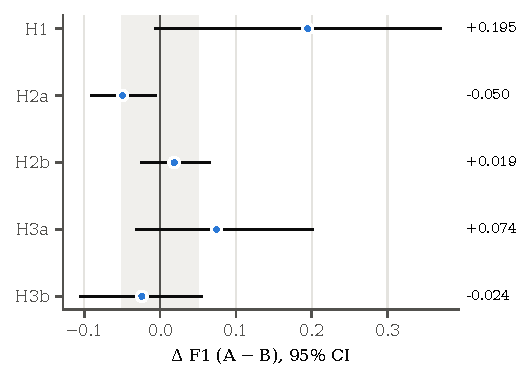
\includegraphics[width=\columnwidth]{figures/fig_confirmatory_D1.pdf}
\caption{Confirmatory F1 differences with 95\% CIs (D1-test, judge M1). Shaded band: the $\pm0.05$ equivalence margin.}\label{fig:forest}
\end{figure}

\begin{figure}[!htb]
\centering
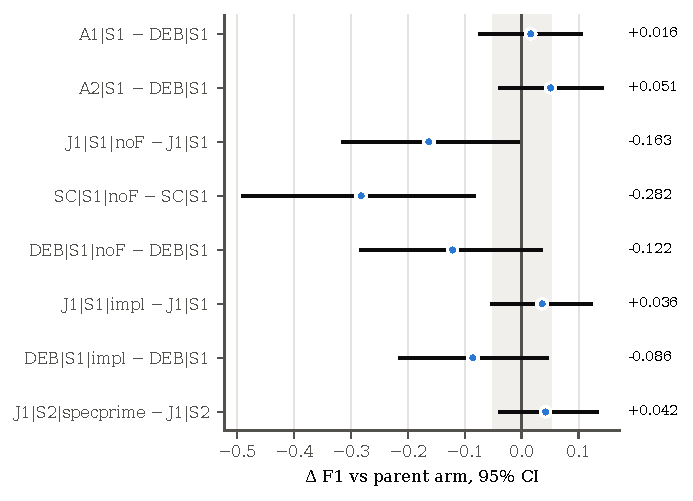
\includegraphics[width=\columnwidth]{figures/fig_e4_ablations_D1.pdf}
\caption{E4: F1 difference of each ablation from its parent arm with 95\% CIs (D1-test, judge M1). Shaded band: $\pm0.05$.}\label{fig:abl}
\end{figure}

\begin{figure*}[!htb]
\centering
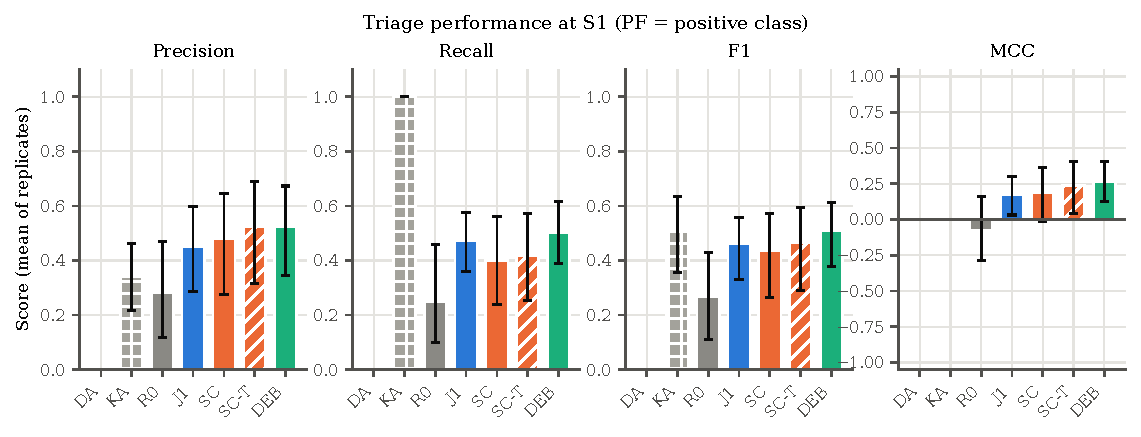
\includegraphics[width=\textwidth]{figures/fig_e1_prf_D1.pdf}
\caption{E1: precision, recall, F1 and MCC at S1 on D1-test (judge M1) with bug-level 95\% CIs. Hatched bars: keep-all (grid) and the token-matched SC-T arm.}\label{fig:prf}
\end{figure*}

\begin{table}[!htb]
\caption{E2: F1 (MCC) by specification level and arm, D1-test, judge M1, mean of \V{frozen:decoding:replicates} replicates. S0: signature; S1: + Javadoc; S2: + inferred specification.}\label{tab:e2}
\footnotesize\setlength{\tabcolsep}{3pt}
\begin{tabular}{@{}l c c c@{}}
\toprule
Level & J1 & SC & DEB \\
\midrule
S0 & \V{d1:J1|S0:f1} (\V{d1:J1|S0:mcc}) & \V{d1:SC|S0:f1} (\V{d1:SC|S0:mcc}) & \V{d1:DEB|S0:f1} (\V{d1:DEB|S0:mcc}) \\
S1 & \V{d1:J1|S1:f1} (\V{d1:J1|S1:mcc}) & \V{d1:SC|S1:f1} (\V{d1:SC|S1:mcc}) & \V{d1:DEB|S1:f1} (\V{d1:DEB|S1:mcc}) \\
S2 & \V{d1:J1|S2:f1} (\V{d1:J1|S2:mcc}) & \V{d1:SC|S2:f1} (\V{d1:SC|S2:mcc}) & \V{d1:DEB|S2:f1} (\V{d1:DEB|S2:mcc}) \\
\bottomrule
\end{tabular}
\end{table}


% (float tab:base is printed in the final paper)


\begin{table*}[!htb]
\caption{E5: F1 (MCC) at S1 by dataset and judge. Baselines do not depend on the judge. D2 F1 is not comparable with D1 F1 (different \PF{} prevalence).}\label{tab:robust}
\footnotesize
\begin{tabular}{@{}l c c c c@{}}
\toprule
 & \multicolumn{2}{c}{D1-test} & \multicolumn{2}{c}{D2 (seeded)} \\
\cmidrule(lr){2-3}\cmidrule(lr){4-5}
Arm & M1 (9B) & M2 (12B) & M1 (9B) & M2 (12B) \\
\midrule
\PF{} prevalence & \multicolumn{2}{c}{\V{sum:prevalence:pf_prevalence}} & \multicolumn{2}{c}{\V{sum2:prevalence:pf_prevalence}} \\
KA & \multicolumn{2}{c}{\V{d1:KA:f1} (\V{d1:KA:mcc})} & \multicolumn{2}{c}{\V{d2:KA:f1} (\V{d2:KA:mcc})} \\
R0 & \multicolumn{2}{c}{\V{d1:R0:f1} (\V{d1:R0:mcc})} & \multicolumn{2}{c}{\V{d2:R0:f1} (\V{d2:R0:mcc})} \\
J1 & \V{d1:J1|S1:f1} (\V{d1:J1|S1:mcc}) & \V{d1m2:J1|S1:f1} (\V{d1m2:J1|S1:mcc}) & \V{d2:J1|S1:f1} (\V{d2:J1|S1:mcc}) & \V{d2m2:J1|S1:f1} (\V{d2m2:J1|S1:mcc}) \\
SC & \V{d1:SC|S1:f1} (\V{d1:SC|S1:mcc}) & \V{d1m2:SC|S1:f1} (\V{d1m2:SC|S1:mcc}) & \V{d2:SC|S1:f1} (\V{d2:SC|S1:mcc}) & \V{d2m2:SC|S1:f1} (\V{d2m2:SC|S1:mcc}) \\
DEB & \V{d1:DEB|S1:f1} (\V{d1:DEB|S1:mcc}) & \V{d1m2:DEB|S1:f1} (\V{d1m2:DEB|S1:mcc}) & \V{d2:DEB|S1:f1} (\V{d2:DEB|S1:mcc}) & \V{d2m2:DEB|S1:f1} (\V{d2m2:DEB|S1:mcc}) \\
\bottomrule
\end{tabular}
\end{table*}


\begin{table*}[!htb]
\caption{How the arms here map to the base papers' approaches. All are re-implemented on this study's evidence package, labels and judge; none uses the original code.}\label{tab:reimpl}
\scriptsize\setlength{\tabcolsep}{2.5pt}
\begin{tabularx}{\textwidth}{@{}>{\raggedright\arraybackslash}p{1.45cm} >{\raggedright\arraybackslash}p{4.2cm} Y@{}}
\toprule
Arm & Original approach & Fidelity (matches / differs / why) \\
\midrule
DA & TestART~\cite{gu2026testart}, ChatAssert~\cite{hayet2025chatassert}, TaRGET~\cite{yaraghi2025target} & \emph{Matches} their premise that a failing test is wrong. \emph{Differs}: no repair step; DA is the limit case, since any repair of a program-fault test removes the bug evidence. \\
R0 & Maddila et al.~\cite{maddila2026agentic}; alarm triage~\cite{herzig2015alarms} & \emph{Matches} rule-based, model-free triage. \emph{Differs}: one rule on failure type and deepest project frame; no reproducibility checks or bisection. \\
DEB & JavaOracle debate~\cite{fu2026javaoracle} & \emph{Matches} adversarial agents and an adjudicator. \emph{Differs}: fixed five-call budget, anonymised random argument order, cited evidence, local 9B judge. \\
SC & JSTestCraft vote~\cite{liu2026jstestcraft}; self-consistency~\cite{wang2023selfconsistency} & \emph{Matches} majority voting. \emph{Differs}: five samples of one model, not three models. \\
VOTE3/5 & JSTestCraft three-LLM vote~\cite{liu2026jstestcraft} & \emph{Matches} a three-family majority. \emph{Differs}: local, budget-matched. E8: F1 \V{e8:summary:VOTE3|S1:f1} vs SC3 \V{e8:summary:SC3|S1:f1}, $\Delta$ \V{e8:hypotheses:H8-1:delta} \V{e8:hypotheses:H8-1:ci95}, $p_\mathrm{Holm}$ \V{e8:hypotheses:H8-1:p_holm}. \\
Zhao et al.\ finding & effective generated tests: \V{cit:zhao lo}--\V{cit:zhao hi}\%\cited{} over six models~\cite{zhao2026misguidance} & \emph{Not replicated} (rule fixed in advance): \V{zhao:subsets:all_D1:share_effective_pct@2}\% \V{zhao:subsets:all_D1:ci95_pct@ci2} effective; the interval overlaps their range, and the qualitative finding (about \V{zhao:subsets:all_D1:share_effective_pct@0}\% of generated tests reveal the bug) holds. \emph{Differs}: one generator vs their six, reconstructed frame, Defects4J~3.0.1. \\
\bottomrule
\end{tabularx}
\end{table*}

\begin{figure*}[t]
\centering
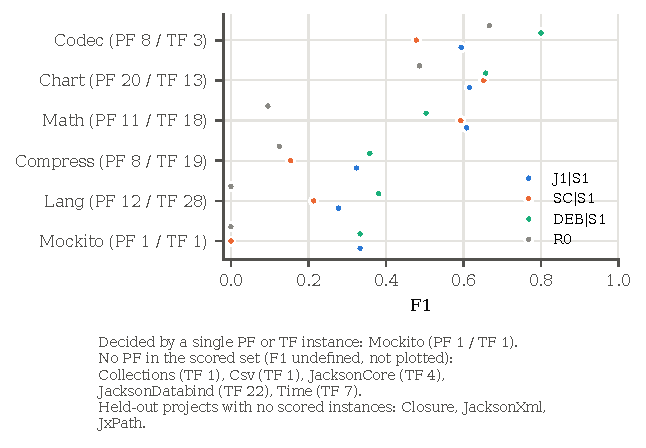
\includegraphics[width=0.8\textwidth]{figures/fig_r5_per_project_D1.pdf}
\caption{Per-project F1 at S1 on D1-test (judge M1), projects with both classes.}\label{fig:perproject}
\end{figure*}

% D-81: not a float, so it stays directly below the Appendix B heading (same numbering and caption style)
\par\medskip\noindent\begin{minipage}{\columnwidth}{\footnotesize\refstepcounter{table}\label{tab:sens}\textbf{Table~\thetable}\enspace Sensitivity of F1 (MCC) at S1, D1-test, judge M1: invalid outputs excluded instead of scored \TF; AMB counted as \PF{} or as \TF.\par}\smallskip
{\noindent \footnotesize
\begin{tabular}{@{}l c c c@{}}
\toprule
Arm & invalid excluded & AMB as \PF & AMB as \TF \\
\midrule
R0 & \V{sum:sensitivity_f1:invalid_excluded:R0:f1} (\V{sum:sensitivity_f1:invalid_excluded:R0:mcc}) & \V{sum:sensitivity_f1:AMB_as_PF:R0:f1} (\V{sum:sensitivity_f1:AMB_as_PF:R0:mcc}) & \V{sum:sensitivity_f1:AMB_as_TF:R0:f1} (\V{sum:sensitivity_f1:AMB_as_TF:R0:mcc}) \\
J1 & \V{sum:sensitivity_f1:invalid_excluded:J1|S1:f1} (\V{sum:sensitivity_f1:invalid_excluded:J1|S1:mcc}) & \V{sum:sensitivity_f1:AMB_as_PF:J1|S1:f1} (\V{sum:sensitivity_f1:AMB_as_PF:J1|S1:mcc}) & \V{sum:sensitivity_f1:AMB_as_TF:J1|S1:f1} (\V{sum:sensitivity_f1:AMB_as_TF:J1|S1:mcc}) \\
SC & \V{sum:sensitivity_f1:invalid_excluded:SC|S1:f1} (\V{sum:sensitivity_f1:invalid_excluded:SC|S1:mcc}) & \V{sum:sensitivity_f1:AMB_as_PF:SC|S1:f1} (\V{sum:sensitivity_f1:AMB_as_PF:SC|S1:mcc}) & \V{sum:sensitivity_f1:AMB_as_TF:SC|S1:f1} (\V{sum:sensitivity_f1:AMB_as_TF:SC|S1:mcc}) \\
DEB & \V{sum:sensitivity_f1:invalid_excluded:DEB|S1:f1} (\V{sum:sensitivity_f1:invalid_excluded:DEB|S1:mcc}) & \V{sum:sensitivity_f1:AMB_as_PF:DEB|S1:f1} (\V{sum:sensitivity_f1:AMB_as_PF:DEB|S1:mcc}) & \V{sum:sensitivity_f1:AMB_as_TF:DEB|S1:f1} (\V{sum:sensitivity_f1:AMB_as_TF:DEB|S1:mcc}) \\
\bottomrule
\end{tabular}
\par}\end{minipage}\par\medskip



% D-81: not a float, so it stays directly below the Appendix B heading (same numbering and caption style)
\par\medskip\noindent\begin{minipage}{\columnwidth}{\footnotesize\refstepcounter{table}\label{tab:cost}\textbf{Table~\thetable}\enspace Cost and latency per arm from the call logs, D1-test, S1, judge M1, \V{cost:scored_instances} scored instances $\times$ \V{cost:arms:DEB:replicates} replicates. Tokens: mean per instance; wall time per instance (calls run one at a time). API cost: zero.\par}\smallskip
{\noindent \footnotesize\setlength{\tabcolsep}{3.5pt}
\begin{tabular}{@{}l c c c c c@{}}
\toprule
Arm & Calls & In tokens & Out tokens & Median (s) & P90 (s) \\
\midrule
J1 & \V{cost:arms:J1:calls_per_instance@0} & \V{cost:arms:J1:input_tokens_per_instance@0} & \V{cost:arms:J1:output_tokens_per_instance@0} & \V{cost:arms:J1:wall_s_median@2} & \V{cost:arms:J1:wall_s_p90@2} \\
SC & \V{cost:arms:SC:calls_per_instance@0} & \V{cost:arms:SC:input_tokens_per_instance@0} & \V{cost:arms:SC:output_tokens_per_instance@0} & \V{cost:arms:SC:wall_s_median@2} & \V{cost:arms:SC:wall_s_p90@2} \\
SC-T & \V{cost:arms:SC-T:calls_per_instance@0} & \V{cost:arms:SC-T:input_tokens_per_instance@0} & \V{cost:arms:SC-T:output_tokens_per_instance@0} & \V{cost:arms:SC-T:wall_s_median@2} & \V{cost:arms:SC-T:wall_s_p90@2} \\
DEB & \V{cost:arms:DEB:calls_per_instance@0} & \V{cost:arms:DEB:input_tokens_per_instance@0} & \V{cost:arms:DEB:output_tokens_per_instance@0} & \V{cost:arms:DEB:wall_s_median@2} & \V{cost:arms:DEB:wall_s_p90@2} \\
\bottomrule
\end{tabular}
\par}\end{minipage}\par\medskip


\paragraph{Failure cases.} Per-project F1 (Appendix~\ref{app:extra}) is lowest on Compress and Lang for DEB (\V{sum:per_project_f1:DEB|S1:Compress} and \V{sum:per_project_f1:DEB|S1:Lang}); a project whose sample holds only test faults, such as JacksonDatabind (\V{sum:per_project_counts:JacksonDatabind:TF} \TF, \V{sum:per_project_counts:JacksonDatabind:PF} \PF), can contribute only false alarms. Of the three program faults in Table~\ref{tab:qual}, \QcaseA{} turns on the expected and actual values in the failure message (cf.\ A4), in \QcaseB{} the judge takes documented buggy behaviour as the contract (cf.\ H2a, A5a), and in \QcaseC{} it inverts the failure evidence, a limit of the small judge.

\section{Post hoc and exploratory analyses}\label{app:explore}
% numbering restarts in each appendix
All analyses here are post hoc (D-80) or exploratory (D-82): their rules were fixed before they were computed, none is a confirmatory test, and none is corrected for multiplicity.

\paragraph{Specification mixed model.} An exploratory mixed model on \PF{} recall, with bug-level cluster-bootstrap intervals (\V{glmmb:B} refits), estimates odds ratios of \V{glmmb:models:PF_recall:terms:1:odds_ratio} \V{glmmb:models:PF_recall:terms:1:or_ci95_bootstrap} for S0 and \V{glmmb:models:PF_recall:terms:2:odds_ratio} \V{glmmb:models:PF_recall:terms:2:or_ci95_bootstrap} for S2 relative to S1; on \TF{} instances the S0 odds ratio is \V{glmmb:models:TF_specificity:terms:1:odds_ratio} \V{glmmb:models:TF_specificity:terms:1:or_ci95_bootstrap}. All three intervals include 1, so the model adds no evidence of a specification effect beyond the contrasts above. Its variational intervals under-covered in simulation, so it is reported only with bootstrap intervals; a population-averaged GEE with bugs as clusters and bias-reduced sandwich errors (sensitivity, D-120) gives \PF{}-recall odds ratios of \V{rv19:mixed_model:gee:PF_recall:terms:1:odds_ratio} \V{rv19:mixed_model:gee:PF_recall:terms:1:or_ci95_robust} for S0 and \V{rv19:mixed_model:gee:PF_recall:terms:2:odds_ratio} \V{rv19:mixed_model:gee:PF_recall:terms:2:or_ci95_robust} for S2, again including 1.

\paragraph{Summary.} The practical takeaway is the cost-ratio break-even: DEB beats keeping every failure only while a missed bug costs less than \V{xd:D1:DEB:breakeven_vs_KA@2} false alarms (\V{xd:D1:DEB:breakeven_vs_KA_natural@2} at the natural prevalence). The practical selective rule is DEB's at $\tau=\V{sel:arms:DEB:tau}$ (tuned on dev): it discards \V{sel:arms:DEB:share_discarded@pct} of failures, loses \V{sel:arms:DEB:pf_lost@1} of \V{sel:arms:DEB:pf_in_set} bugs per replicate and gains \V{sel:arms:DEB:delta_f1_vs_ka} F1 over keep-all (\V{sel:arms:DEB:delta_f1_vs_ka_ci95}); SC's rule at $\tau=\V{sel:arms:SC:tau}$ discards more but loses \V{sel:arms:SC:pf_lost@0} of \V{sel:arms:SC:pf_in_set} bugs (Table~\ref{tab:selka}). SC's rule did not transfer to the third-family judge (H6-3 \V{e6b:hypotheses:H6-3:delta}, not supported), and DEB's has been evaluated on M1 only. The judges are overconfident (DEB: stated confidence \V{xd:D2:calibration:DEB:mean_confidence@2}, accuracy \V{xd:D2:calibration:DEB:accuracy@2}), and escalating split SC votes to DEB did not beat DEB alone.

\paragraph{Development gate versus held-out result.} M1's one-shot F1 was far below R0's on the development pilot (\V{devgate:G_d_detail:J1_f1} vs \V{devgate:G_d_detail:R0_f1}; \V{devgate:n_instances} instances) and above it on the held-out split (\V{d1:J1|S1:f1} vs \V{d1:R0:f1}); with \V{devgate:n_bugs} bugs the pilot's interval, \V{devgate:G_d_detail:delta_ci95_bug_bootstrap}, spanned both, so the gate measured project composition more than judge quality.

\par\medskip\noindent\begin{minipage}{\columnwidth}{\footnotesize\refstepcounter{table}\label{tab:mde}\textbf{Table~\thetable}\enspace Post hoc sensitivity analysis (not observed power): minimum detectable $\Delta$F1 at \V{mde:power@pct0} power, $\mathrm{MDE}=(z_{1-\alpha/2}+z_{\V{mde:power@1}})\,\mathrm{SE}$, SE: standard deviation of the bug-level bootstrap $\Delta$F1, at $\alpha=\V{mde:alpha@2}$ and at the Holm $\alpha$ for the smallest $p$ (\V{mde:alpha_holm_smallest_p@2}).\par}\smallskip
{\noindent \footnotesize\setlength{\tabcolsep}{3.5pt}
\begin{tabular}{@{}l c c c c c@{}}
\toprule
H & $n$ (bugs) & $\Delta$F1 & SE & MDE$_{\V{mde:alpha@2}}$ & MDE$_{\V{mde:alpha_holm_smallest_p@2}}$ \\
\midrule
H1 & \V{mde:tests:H1:n_instances} (\V{mde:tests:H1:n_bugs}) & \V{mde:tests:H1:delta} & \V{mde:tests:H1:se_bootstrap} & \V{mde:tests:H1:mde_alpha_005} & \V{mde:tests:H1:mde_alpha_holm_min} \\
H2a & \V{mde:tests:H2a:n_instances} (\V{mde:tests:H2a:n_bugs}) & \V{mde:tests:H2a:delta} & \V{mde:tests:H2a:se_bootstrap} & \V{mde:tests:H2a:mde_alpha_005} & \V{mde:tests:H2a:mde_alpha_holm_min} \\
H2b & \V{mde:tests:H2b:n_instances} (\V{mde:tests:H2b:n_bugs}) & \V{mde:tests:H2b:delta} & \V{mde:tests:H2b:se_bootstrap} & \V{mde:tests:H2b:mde_alpha_005} & \V{mde:tests:H2b:mde_alpha_holm_min} \\
H3a & \V{mde:tests:H3a:n_instances} (\V{mde:tests:H3a:n_bugs}) & \V{mde:tests:H3a:delta} & \V{mde:tests:H3a:se_bootstrap} & \V{mde:tests:H3a:mde_alpha_005} & \V{mde:tests:H3a:mde_alpha_holm_min} \\
H3b & \V{mde:tests:H3b:n_instances} (\V{mde:tests:H3b:n_bugs}) & \V{mde:tests:H3b:delta} & \V{mde:tests:H3b:se_bootstrap} & \V{mde:tests:H3b:mde_alpha_005} & \V{mde:tests:H3b:mde_alpha_holm_min} \\
\bottomrule
\end{tabular}
\par}\end{minipage}\par\medskip
\par\medskip\noindent\begin{minipage}{\columnwidth}{\footnotesize\refstepcounter{figure}\label{fig:spec}\textbf{Fig.~\thefigure}\enspace E2: F1 by specification level for J1, SC and DEB on D1-test (judge M1), bug-level 95\% CIs.\par}\smallskip
{\noindent\centering 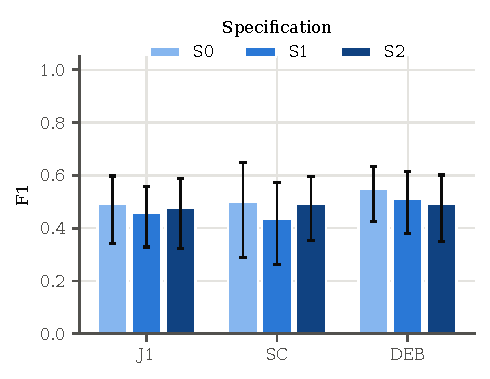
\includegraphics[width=0.8\columnwidth]{figures/fig_e2_spec_f1_D1.pdf}
\par}\end{minipage}\par\medskip
\par\medskip\noindent\begin{minipage}{\columnwidth}{\footnotesize\refstepcounter{figure}\label{fig:pareto}\textbf{Fig.~\thefigure}\enspace E3: F1 against consumed tokens per instance at S1 (D1-test, judge M1), bug-level 95\% CIs.\par}\smallskip
{\noindent\centering 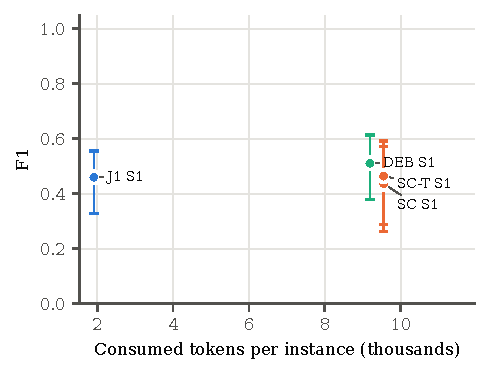
\includegraphics[width=0.85\columnwidth]{figures/fig_e3_pareto_D1.pdf}
\par}\end{minipage}\par\medskip
\par\medskip\noindent\begin{minipage}{\columnwidth}{\footnotesize\refstepcounter{table}\label{tab:explore}\textbf{Table~\thetable}\enspace Exploratory analyses (D-82), D1-test, S1, judge M1. $r$: cost of a missed bug in false alarms. $\tau$: confidence threshold tuned on the development pilot only. Bug-level 95\% CIs; no correction.\par}\smallskip
{\noindent\scriptsize\setlength{\tabcolsep}{2.5pt}
\begin{tabularx}{\columnwidth}{@{}Y >{\raggedright\arraybackslash}p{3.45cm}@{}}
\toprule
Quantity & Value \\
\midrule
Cost ratio: DEB cheaper than KA iff $r<$ & \V{xd:D1:DEB:breakeven_vs_KA@2} (natural \V{xd:D1:DEB:breakeven_vs_KA_natural@2}) \\
Cost ratio: DEB cheaper than DA iff $r>$ & \V{xd:D1:DEB:breakeven_vs_DA@2} (natural \V{xd:D1:DEB:breakeven_vs_DA_natural@2}) \\
Cost ratio: J1 / SC cheaper than KA iff $r<$ & \V{xd:D1:J1:breakeven_vs_KA@2} / \V{xd:D1:SC:breakeven_vs_KA@2} \\
ECE: J1 / SC / DEB & \V{xd:D2:calibration:J1:ece} / \V{xd:D2:calibration:SC:ece} / \V{xd:D2:calibration:DEB:ece} \\
DEB mean confidence vs accuracy & \V{xd:D2:calibration:DEB:mean_confidence} vs \V{xd:D2:calibration:DEB:accuracy} \\
Selective SC ($\tau$=\V{xd:D2:selective:SC:tau}): F1, $\Delta$F1 & \V{xd:D2:selective:SC:f1}, \V{xd:D2:selective:SC:delta_f1} \V{xd:D2:selective:SC:delta_f1_ci95} \\
Selective J1 ($\tau$=\V{xd:D2:selective:J1:tau}): F1, $\Delta$F1 & \V{xd:D2:selective:J1:f1}, \V{xd:D2:selective:J1:delta_f1} \V{xd:D2:selective:J1:delta_f1_ci95} \\
Selective DEB ($\tau$=\V{xd:D2:selective:DEB:tau}): F1, $\Delta$F1 & \V{xd:D2:selective:DEB:f1}, \V{xd:D2:selective:DEB:delta_f1} \V{xd:D2:selective:DEB:delta_f1_ci95} \\
SC$\to$DEB cascade: escalated / F1 & \V{xd:D3:escalation_rate@pct} / \V{xd:D3:f1} \\
Cascade $-$ SC; $-$ DEB ($\Delta$F1) & \V{xd:D3:vs_SC:delta} \V{xd:D3:vs_SC:ci95}; \V{xd:D3:vs_DEB:delta} \V{xd:D3:vs_DEB:ci95} \\
Cascade tokens (SC / DEB) & \V{xd:D3:tokens_per_instance@0} (\V{xd:D3:sc_tokens_per_instance@0} / \V{xd:D3:deb_tokens_per_instance@0}) \\
Concession rate, round 1 / 2 & \V{xd:D4:concession_rate_r1@pct} / \V{xd:D4:concession_rate_r2@pct} \\
Sided with last-presented ($p$ vs 0.5) & \V{xd:D4:last_presented_share@pct} (\V{xd:D4:last_presented_p}) \\
DEB differs from SC majority; DEB right then & \V{xd:D4:flip_rate_vs_sc_majority@pct}; \V{xd:D4:deb_correct_share_among_flips@pct} \\
\bottomrule
\end{tabularx}
\par}\end{minipage}\par\medskip
\par\medskip\noindent\begin{minipage}{\columnwidth}{\footnotesize\refstepcounter{table}\label{tab:selka}\textbf{Table~\thetable}\enspace Selective triage against keep-all (exploratory, D-82), D1-test, S1, judge M1: discard only a TF stated with confidence $\geq\tau$ ($\tau$ tuned on the development pilot). Lost: PF tests discarded per replicate, of the PF instances in the set. The arm's own MCC is shown on its own (keep-all's MCC is 0).\par}\smallskip
{\noindent\scriptsize\setlength{\tabcolsep}{2.5pt}
\resizebox{\columnwidth}{!}{\begin{tabular}{@{}l c c c c c@{}}
\toprule
Arm & $\tau$ & $\Delta$F1 vs KA [95\% CI] & Lost & Discarded & MCC [95\% CI] \\
\midrule
DEB & \V{sel:arms:DEB:tau} & \V{sel:arms:DEB:delta_f1_vs_ka} \V{sel:arms:DEB:delta_f1_vs_ka_ci95} & \V{sel:arms:DEB:pf_lost@1} / \V{sel:arms:DEB:pf_in_set} & \V{sel:arms:DEB:share_discarded@pct} & \V{sel:arms:DEB:mcc} \V{sel:arms:DEB:mcc_ci95} \\
J1 & \V{sel:arms:J1:tau} & \V{sel:arms:J1:delta_f1_vs_ka} \V{sel:arms:J1:delta_f1_vs_ka_ci95} & \V{sel:arms:J1:pf_lost@1} / \V{sel:arms:J1:pf_in_set} & \V{sel:arms:J1:share_discarded@pct} & \V{sel:arms:J1:mcc} \V{sel:arms:J1:mcc_ci95} \\
SC & \V{sel:arms:SC:tau} & \V{sel:arms:SC:delta_f1_vs_ka} \V{sel:arms:SC:delta_f1_vs_ka_ci95} & \V{sel:arms:SC:pf_lost@1} / \V{sel:arms:SC:pf_in_set} & \V{sel:arms:SC:share_discarded@pct} & \V{sel:arms:SC:mcc} \V{sel:arms:SC:mcc_ci95} \\
\bottomrule
\end{tabular}}
\par}\end{minipage}\par\medskip

\section{Further judges, the vote and a frontier reference (E6, E8, E9)}\label{app:post}
% numbering restarts in each appendix

\noindent\textit{Second judge (M2), detail.} On the same instances, M2 (12B) improved on M1 in every arm and dataset: on D1-test by \V{r3:D1:m2_minus_m1:J1:f1:delta} (J1), \V{r3:D1:m2_minus_m1:SC:f1:delta} (SC) and \V{r3:D1:m2_minus_m1:DEB:f1:delta} (DEB, 95\% CI \V{r3:D1:m2_minus_m1:DEB:f1:ci95}), and on D2 by \V{r3:D2:m2_minus_m1:J1:f1:delta}, \V{r3:D2:m2_minus_m1:SC:f1:delta} and \V{r3:D2:m2_minus_m1:DEB:f1:delta}. DEB ranks first by F1 and MCC under M2 on both datasets. M2's samples were almost unanimous, so its SC reproduced J1's F1 on D1-test. M2 shares the generator's family, so self-preference cannot be excluded.

Run after the primary results under rules fixed before any call (D-82, D-83; builds D-85, D-88, D-90): D1-test, S1, frozen prompts and decoding, one replicate, bug-level 95\% CIs. E6b and E8 test hypotheses fixed in advance with Holm within each family; E6a is exploratory. The E6b judge (Ministral~3 14B, neither Qwen nor Gemma) was the first of four candidates fixed in advance to pass Step~1 and gates G-a/G-b on the development pilot. VOTE3 is a majority of one fresh J1 call each from M1, M2 and E6b; VOTE5 of 2+2+1 further calls; SC3 is the majority of the first three of M1's committed SC samples.

\par\medskip\noindent\begin{minipage}{\columnwidth}{\footnotesize\refstepcounter{table}\label{tab:post}\textbf{Table~\thetable}\enspace E6b, E6a and E8 on D1-test, S1 (\V{e6b:n_instances} instances, \V{e6b:n_bugs} bugs); one replicate (M1: three). $\Delta$: paired difference, bug-level 95\% CI; $p_\mathrm{H}$: Holm within E6b or E8; H6-3 at the frozen $\tau=\V{e6b:hypotheses:H6-3:tau}$.\par}\smallskip
{\noindent\scriptsize\setlength{\tabcolsep}{4pt}
\resizebox{\columnwidth}{!}{\begin{tabular}{@{}l l r@{}}
\toprule
Quantity & Estimate [95\% CI] & $p_\mathrm{H}$ \\
\midrule
E6b F1: J1 / SC / DEB & \V{e6b:summary:J1:f1} / \V{e6b:summary:SC:f1} / \V{e6b:summary:DEB:f1} &  \\
E6b MCC: J1 / SC / DEB & \V{e6b:summary:J1:mcc} / \V{e6b:summary:SC:mcc} / \V{e6b:summary:DEB:mcc} &  \\
H6-1 $\Delta$F1 DEB$-$SC & \V{e6b:hypotheses:H6-1:delta} \V{e6b:hypotheses:H6-1:ci95} & \V{e6b:hypotheses:H6-1:p_holm} \\
H6-2 MCC(DEB) & \V{e6b:hypotheses:H6-2:mcc} \V{e6b:hypotheses:H6-2:ci95} & \V{e6b:hypotheses:H6-2:p_holm} \\
H6-3 selective SC$-$SC & \V{e6b:hypotheses:H6-3:delta} \V{e6b:hypotheses:H6-3:ci95} & -- \\
DEB $\Delta$F1 E6b$-$M2 & \V{e6b:family_check:e6b_minus:DEB E6B-M2:f1:delta} \V{e6b:family_check:e6b_minus:DEB E6B-M2:f1:ci95} &  \\
DEB $\Delta$F1 E6b$-$M1 & \V{e6b:family_check:e6b_minus:DEB E6B-M1:f1:delta} \V{e6b:family_check:e6b_minus:DEB E6B-M1:f1:ci95} &  \\
E6a 35B F1: J1 / DEB & \V{e6a:summary:35B:J1:f1} / \V{e6a:summary:35B:DEB:f1} &  \\
E6a DEB $\Delta$F1 35B$-$M1 & \V{e6a:35b_minus:DEB 35B-M1:f1:delta} \V{e6a:35b_minus:DEB 35B-M1:f1:ci95} &  \\
E8 F1: VOTE3 / VOTE5 & \V{e8:summary:VOTE3|S1:f1} / \V{e8:summary:VOTE5|S1:f1} &  \\
E8 MCC: VOTE3 / VOTE5 & \V{e8:summary:VOTE3|S1:mcc} / \V{e8:summary:VOTE5|S1:mcc} &  \\
M1 F1: SC3 / SC / DEB & \V{e8:summary:SC3|S1:f1} / \V{e8:summary:SC|S1:f1} / \V{e8:summary:DEB|S1:f1} &  \\
H8-1 VOTE3$-$SC3 & \V{e8:hypotheses:H8-1:delta} \V{e8:hypotheses:H8-1:ci95} & \V{e8:hypotheses:H8-1:p_holm} \\
H8-2 VOTE5$-$SC & \V{e8:hypotheses:H8-2:delta} \V{e8:hypotheses:H8-2:ci95} & \V{e8:hypotheses:H8-2:p_holm} \\
H8-3 VOTE5$-$DEB & \V{e8:hypotheses:H8-3:delta} \V{e8:hypotheses:H8-3:ci95} & \V{e8:hypotheses:H8-3:p_holm} \\
PF lost: VOTE3 / 5, SC, DEB & \V{e8:summary:VOTE3|S1:pf_lost@0} / \V{e8:summary:VOTE5|S1:pf_lost@0}, \V{e8:summary:SC|S1:pf_lost@0}, \V{e8:summary:DEB|S1:pf_lost@0} of \V{e6b:pf_prevalence:PF} &  \\
\bottomrule
\end{tabular}}
\par}\end{minipage}\par\medskip


\par\medskip\noindent\begin{minipage}{\columnwidth}{\footnotesize\refstepcounter{table}\label{tab:noise}\textbf{Table~\thetable}\enspace Replicate noise (exploratory, D-94): M1's three replicates scored separately at S1 on the \V{rn:n_instances} D1-test instances, against the single-replicate cross-model differences. A difference is \emph{beyond} M1's spread when $|\Delta|$ exceeds the range of M1's replicates for the arm compared. No test.\par}\smallskip
{\noindent\scriptsize\setlength{\tabcolsep}{4pt}
\resizebox{\columnwidth}{!}{\begin{tabular}{@{}l l c c c@{}}
\toprule
M1 arm & F1 per replicate & F1 range & F1 SD & MCC range \\
\midrule
J1 & \V{rn:noise:J1:f1:per_replicate:0} / \V{rn:noise:J1:f1:per_replicate:1} / \V{rn:noise:J1:f1:per_replicate:2} & \V{rn:noise:J1:f1:range} & \V{rn:noise:J1:f1:sd} & \V{rn:noise:J1:mcc:range} \\
SC & \V{rn:noise:SC:f1:per_replicate:0} / \V{rn:noise:SC:f1:per_replicate:1} / \V{rn:noise:SC:f1:per_replicate:2} & \V{rn:noise:SC:f1:range} & \V{rn:noise:SC:f1:sd} & \V{rn:noise:SC:mcc:range} \\
SC-T & \V{rn:noise:SC-T:f1:per_replicate:0} / \V{rn:noise:SC-T:f1:per_replicate:1} / \V{rn:noise:SC-T:f1:per_replicate:2} & \V{rn:noise:SC-T:f1:range} & \V{rn:noise:SC-T:f1:sd} & \V{rn:noise:SC-T:mcc:range} \\
DEB & \V{rn:noise:DEB:f1:per_replicate:0} / \V{rn:noise:DEB:f1:per_replicate:1} / \V{rn:noise:DEB:f1:per_replicate:2} & \V{rn:noise:DEB:f1:range} & \V{rn:noise:DEB:f1:sd} & \V{rn:noise:DEB:mcc:range} \\
SC3 & \V{rn:noise:SC3:f1:per_replicate:0} / \V{rn:noise:SC3:f1:per_replicate:1} / \V{rn:noise:SC3:f1:per_replicate:2} & \V{rn:noise:SC3:f1:range} & \V{rn:noise:SC3:f1:sd} & \V{rn:noise:SC3:mcc:range} \\
\midrule
Difference (F1) & $\Delta$ & M1 range & & \\
\midrule
J1: M2$-$M1 & \V{rn:cross_model:0:delta} & \V{rn:cross_model:0:m1_range} & beyond & \\
SC: M2$-$M1 & \V{rn:cross_model:2:delta} & \V{rn:cross_model:2:m1_range} & beyond & \\
DEB: M2$-$M1 & \V{rn:cross_model:4:delta} & \V{rn:cross_model:4:m1_range} & within & \\
J1: E6b$-$M1 & \V{rn:cross_model:1:delta} & \V{rn:cross_model:1:m1_range} & beyond & \\
SC: E6b$-$M1 & \V{rn:cross_model:3:delta} & \V{rn:cross_model:3:m1_range} & beyond & \\
DEB: E6b$-$M1 & \V{rn:cross_model:5:delta} & \V{rn:cross_model:5:m1_range} & within & \\
J1: 35B$-$M1 & \V{rn:cross_model:6:delta} & \V{rn:cross_model:6:m1_range} & beyond & \\
DEB: 35B$-$M1 & \V{rn:cross_model:7:delta} & \V{rn:cross_model:7:m1_range} & within & \\
VOTE3$-$SC3 & \V{rn:cross_model:8:delta} & \V{rn:cross_model:8:m1_range} & beyond & \\
VOTE5$-$SC & \V{rn:cross_model:9:delta} & \V{rn:cross_model:9:m1_range} & beyond & \\
VOTE5$-$DEB & \V{rn:cross_model:10:delta} & \V{rn:cross_model:10:m1_range} & within & \\
\bottomrule
\end{tabular}}
\par}\end{minipage}\par\medskip


\par\medskip\noindent\begin{minipage}{\columnwidth}{\footnotesize\refstepcounter{table}\label{tab:gap}\textbf{Table~\thetable}\enspace Why our numbers differ from the base papers, and where they agree. * taken from the paper.\par}\smallskip
{\noindent\scriptsize\setlength{\tabcolsep}{2.5pt}
\begin{tabularx}{\columnwidth}{@{}>{\raggedright\arraybackslash}p{1.35cm} Y Y@{}}
\toprule
Paper & Differs from ours in & Agrees with ours on \\
\midrule
Zhao et al.~\cite{zhao2026misguidance} & six API generators vs one local; Defects4J~3.0 vs 3.0.1; reconstructed frame & effective-test share: \V{zhao:subsets:all_D1:share_effective_pct@2}\% \V{zhao:subsets:all_D1:ci95_pct@ci2} overlaps \V{cit:zhao lo}--\V{cit:zhao hi}\%\cited \\
JSTestCraft~\cite{liu2026jstestcraft} & JavaScript; recall from a small manual audit; API models; three-model vote inside generation & a cross-family vote keeps recall high: \V{e8:summary:VOTE3|S1:recall} vs \V{cit:jstestcraft recall}\%\cited \\
JavaOracle~\cite{fu2026javaoracle} & oracle generation, not triage; precision on its own labels; API models; debate ablated, not budget-matched & debate trades away true positives: DEB discards \V{d1:DEB|S1:pf_lost@0} of \V{sum:prevalence:PF}; theirs fall \V{cit:javaoracle tp before} to \V{cit:javaoracle tp after}\cited \\
MACO, TestART, CANDOR~\cite{xie2026maco,gu2026testart,xu2026candor} & generation metrics (coverage, pass rate, oracle correctness) on the current version; no prevalence of faults & none directly: no triage result \\
\bottomrule
\end{tabularx}
\par}\end{minipage}\par\medskip


\par\medskip\noindent\begin{minipage}{\columnwidth}{\footnotesize\refstepcounter{table}\label{tab:e9}\textbf{Table~\thetable}\enspace E9, frontier reference point, not a protocol replication (D-92, D-97): Claude Sonnet~5.5 through the Message Batches API on the \V{e9:n_instances} scored D1-test instances; J1 one replicate, DEB three; default sampling, no seeds, thinking off; spend US\$\,\V{e9:spend_usd@2}.\par}\smallskip
{\noindent\scriptsize\setlength{\tabcolsep}{4pt}
\resizebox{\columnwidth}{!}{\begin{tabular}{@{}l l r@{}}
\toprule
Quantity & Estimate [95\% CI] & $p_\mathrm{H}$ \\
\midrule
Sonnet F1: J1 / DEB & \V{e9:summary:J1|S1|SON:f1} / \V{e9:summary:DEB|S1|SON:f1} & \\
Sonnet MCC: J1 / DEB & \V{e9:summary:J1|S1|SON:mcc} / \V{e9:summary:DEB|S1|SON:mcc} & \\
H9-1 $\Delta$F1 DEB$-$J1 & \V{e9:hypotheses:H9-1:delta} \V{e9:hypotheses:H9-1:ci95} & \V{e9:hypotheses:H9-1:p_holm} \\
H9-2 MCC(DEB) & \V{e9:hypotheses:H9-2:mcc} \V{e9:hypotheses:H9-2:ci95} & \V{e9:hypotheses:H9-2:p_holm} \\
DEB $\Delta$F1 Sonnet$-$M1 & \V{e9:sonnet_minus_m1:DEB:f1:delta} \V{e9:sonnet_minus_m1:DEB:f1:ci95} & \\
J1 $\Delta$F1 Sonnet$-$M1 & \V{e9:sonnet_minus_m1:J1:f1:delta} \V{e9:sonnet_minus_m1:J1:f1:ci95} & \\
DEB F1 per replicate: Sonnet & \V{e9:deb_run_to_run_spread:sonnet:f1:per_replicate:0} / \V{e9:deb_run_to_run_spread:sonnet:f1:per_replicate:1} / \V{e9:deb_run_to_run_spread:sonnet:f1:per_replicate:2} & \\
DEB F1 per replicate: M1 & \V{e9:deb_run_to_run_spread:m1:f1:per_replicate:0} / \V{e9:deb_run_to_run_spread:m1:f1:per_replicate:1} / \V{e9:deb_run_to_run_spread:m1:f1:per_replicate:2} & \\
PF lost: Sonnet J1 / DEB; M1 DEB & \V{e9:summary:J1|S1|SON:pf_lost@0} / \V{e9:summary:DEB|S1|SON:pf_lost@1}; \V{e9:summary:DEB|S1:pf_lost@0} & \\
\bottomrule
\end{tabular}}
\par}\end{minipage}\par\medskip

\noindent\textit{Reading.} The third-family judge confirms that DEB is above chance (H6-2) but not that it beats SC (H6-1); the selective rule did not transfer (H6-3). M2, which shares the generator's family, scored above E6b in every arm, consistent with family affinity but confounded with model and size. The vote's gains over SC3 and SC were not significant after Holm, but it lost far fewer bug-revealing tests. The frontier judge is a reference point, not a replication: it shows how much of the gap to the base papers a larger model closes, and its three DEB replicates vary far less than M1's. Its training data very likely include Defects4J and its fixes, so its D1 score may be inflated by memorisation; E9b (D-104) judged the D2 seeded faults, whose fixes no model can have seen, and found no drop (Appendix~\ref{app:cascade}). \textit{Disclosures.} The E6b gate script first crashed on a leakage-abort bookkeeping gap and was fixed before any gate value was seen (D-86); a unit test made \V{q87:calls} unplanned calls by a non-selected candidate on D1-test, quarantined unread and excluded (D-87); E6a's SC was stopped by the memory rule after \V{x35o:decisions_by_arm:SC} decisions and not retried (D-89). A zero-call check found \V{gtr:signals:union} of \V{gtr:generations} generations (\V{gtr:union_share@pct}) cut off by length, so a larger generation context is not justified (D-91). The second-generator selection script crashed on \V{e7a:tried:1:unparseable_classes} generated classes with unbalanced braces and was fixed, counting them as generated but not executed, before that candidate's values were computed (D-102); neither candidate passed, so E7a was not run.
\section{Keep unless unanimous, KUU-NG, escalation and the memorisation check (D-95, D-104, D-105, D-109)}\label{app:cascade}
% numbering restarts in each appendix

\noindent\textit{Error diversity, detail.} On D2 the judges' miss rates on \PF{} ranged from \V{ed:D2:miss_rate:M2:est} to \V{ed:D2:miss_rate:M1:est}. Two families miss the same \PF{} test \V{ed:D2:comparison:mean_cross_family_lift@1} times as often as independence predicts, but three samples of one model do so \V{ed:D2:comparison:mean_within_family_lift@1} times as often (difference \V{ed:D2:comparison:difference_ci95@ci2}); KUU lost \V{ed:D2:kuu_loss:observed@0} tests where unanimity among three samples of M1 or M2 would have lost \V{ed:D2:within_family:M1:unanimous_loss@0} and \V{ed:D2:within_family:M2:unanimous_loss@0}. The diversity is partial: independence would predict \V{ed:D2:kuu_loss:independence_prediction@2} losses. On D1 (post hoc) the criterion fixed in advance is not met, because KUU's single loss ties M2's within-family one; the contrast is model versus resample, not family versus family (Appendix~\ref{app:review}).


\noindent The cascade and the error-diversity analysis were fixed in advance in the version-controlled decision log (D-105) before any E9b call; E9b was fixed in D-104. D2 results are the reads fixed in advance; D1 results are post hoc (development evidence). The frontier tier is a frontier reference point, not a protocol replication.

\par\medskip\noindent\begin{minipage}{\columnwidth}{\footnotesize\refstepcounter{table}\label{tab:cascade}\textbf{Table~\thetable}\enspace D2 seeded faults (\V{cas2:n_instances} instances, \V{cas2:n_bugs} bugs, S1): the cascade against its parts. Sonnet arms one replicate (E9b, US\$\,\V{e9b:spend_usd@2}); M1 DEB is the committed D2 run.\par}\smallskip
{\noindent\scriptsize\setlength{\tabcolsep}{3pt}
\resizebox{\columnwidth}{!}{\begin{tabular}{@{}l r r r r r@{}}
\toprule
Rule & F1 & MCC & Precision & Recall & \PF{} lost \\
\midrule
Cascade (KUU + Sonnet DEB) & \V{cas2:summary:CAS|S1:f1} & \V{cas2:summary:CAS|S1:mcc} & \V{cas2:summary:CAS|S1:precision} & \V{cas2:summary:CAS|S1:recall} & \V{cas2:summary:CAS|S1:pf_lost@0} \\
Cascade to Sonnet J1 & \V{cas2:summary:CASJ1|S1:f1} & \V{cas2:summary:CASJ1|S1:mcc} & \V{cas2:summary:CASJ1|S1:precision} & \V{cas2:summary:CASJ1|S1:recall} & \V{cas2:summary:CASJ1|S1:pf_lost@0} \\
KUU (Tier 1 only) & \V{cas2:summary:KUU|S1:f1} & \V{cas2:summary:KUU|S1:mcc} & \V{cas2:summary:KUU|S1:precision} & \V{cas2:summary:KUU|S1:recall} & \V{cas2:summary:KUU|S1:pf_lost@0} \\
Sonnet DEB, every instance & \V{cas2:summary:DEB|S1|SON:f1} & \V{cas2:summary:DEB|S1|SON:mcc} & \V{cas2:summary:DEB|S1|SON:precision} & \V{cas2:summary:DEB|S1|SON:recall} & \V{cas2:summary:DEB|S1|SON:pf_lost@0} \\
Sonnet J1, every instance & \V{cas2:summary:J1|S1|SON:f1} & \V{cas2:summary:J1|S1|SON:mcc} & \V{cas2:summary:J1|S1|SON:precision} & \V{cas2:summary:J1|S1|SON:recall} & \V{cas2:summary:J1|S1|SON:pf_lost@0} \\
M1 DEB & \V{cas2:summary:DEB|S1:f1} & \V{cas2:summary:DEB|S1:mcc} & \V{cas2:summary:DEB|S1:precision} & \V{cas2:summary:DEB|S1:recall} & \V{cas2:summary:DEB|S1:pf_lost@0} \\
\midrule
\multicolumn{6}{@{}l}{Escalated \V{cas2:escalation:escalated@0} (\V{cas2:escalation:share_escalated@pct1}); Tier 1 discarded \V{cas2:escalation:tier1_discard@0}, kept \V{cas2:escalation:tier1_keep@0}; frontier calls \V{cas2:escalation:frontier_calls_cascade_per_replicate@0} vs \V{cas2:escalation:frontier_calls_all_per_replicate@0}.} \\
\multicolumn{6}{@{}l}{H12-1 $\Delta$MCC \V{cas2:hypotheses:H12-1:delta} \V{cas2:hypotheses:H12-1:ci95}, $p_\mathrm{H}$ \V{cas2:hypotheses:H12-1:p_holm}; H12-2 $\Delta$F1 \V{cas2:hypotheses:H12-2:delta}, 90\% CI \V{cas2:hypotheses:H12-2:ci90}, $p_\mathrm{H}$ \V{cas2:hypotheses:H12-2:p_holm}.} \\
\multicolumn{6}{@{}l}{D1 post hoc (E8 votes + E9 DEB, three replicates): F1 \V{cas1:summary:CAS|S1:f1}, MCC \V{cas1:summary:CAS|S1:mcc}, \PF{} lost \V{cas1:summary:CAS|S1:pf_lost@1}, escalated \V{cas1:escalation:share_escalated@pct0}.} \\
\bottomrule
\end{tabular}}
\par}\end{minipage}\par\medskip

\par\medskip\noindent\begin{minipage}{\columnwidth}{\footnotesize\refstepcounter{table}\label{tab:diversity}\textbf{Table~\thetable}\enspace Error diversity on \PF{} instances (D-105): miss rate per judge, lift = co-error over the independence prediction (mean over pairs), and three-vote unanimous losses. Within-family: the first three of each judge's five SC samples (no E6b SC run exists on D2).\par}\smallskip
{\noindent\scriptsize\setlength{\tabcolsep}{3pt}
\resizebox{\columnwidth}{!}{\begin{tabular}{@{}l r r@{}}
\toprule
Quantity & D2 (fixed in advance) & D1 (post hoc) \\
\midrule
Miss rate M1 / M2 / E6b & \V{ed:D2:miss_rate:M1:est} / \V{ed:D2:miss_rate:M2:est} / \V{ed:D2:miss_rate:E6B:est} & \V{ed:D1:miss_rate:M1:est} / \V{ed:D1:miss_rate:M2:est} / \V{ed:D1:miss_rate:E6B:est} \\
Lift, cross-family & \V{ed:D2:comparison:mean_cross_family_lift@2} & \V{ed:D1:comparison:mean_cross_family_lift@2} \\
Lift, within-family & \V{ed:D2:comparison:mean_within_family_lift@2} & \V{ed:D1:comparison:mean_within_family_lift@2} \\
Difference [95\% CI] & \V{ed:D2:comparison:difference@2} \V{ed:D2:comparison:difference_ci95@ci2} & \V{ed:D1:comparison:difference@2} \V{ed:D1:comparison:difference_ci95@ci2} \\
KUU loss (observed / independent) & \V{ed:D2:kuu_loss:observed@0} / \V{ed:D2:kuu_loss:independence_prediction@2} & \V{ed:D1:kuu_loss:observed@0} / \V{ed:D1:kuu_loss:independence_prediction@2} \\
Within-family unanimous loss M1 / M2 & \V{ed:D2:within_family:M1:unanimous_loss@0} / \V{ed:D2:within_family:M2:unanimous_loss@0} & \V{ed:D1:within_family:M1:unanimous_loss@0} / \V{ed:D1:within_family:M2:unanimous_loss@0} \\
\bottomrule
\end{tabular}}
\par}\end{minipage}\par\medskip

\par\medskip\noindent\begin{minipage}{\columnwidth}{\footnotesize\refstepcounter{table}\label{tab:kuung}\textbf{Table~\thetable}\enspace KUU-NG (D-109): M1, E6b and Llama~3.1 8B (\texttt{\V{kuungsel:selected}}) with fresh J1 calls at S1 (one replicate) against KUU, the M1 + E6b pair and M1 DEB on the same instances. Lost: \PF{} tests; bugs: bugs with no \PF{} test kept. D1 is the data the rule came from.\par}\smallskip
{\noindent\scriptsize\setlength{\tabcolsep}{3pt}
\resizebox{\columnwidth}{!}{\begin{tabular}{@{}l r r r r r r r r@{}}
\toprule
 & \multicolumn{4}{c}{D2 (\V{kuung:D2:n_instances} inst.)} & \multicolumn{4}{c}{D1-test (\V{kuung:D1:n_instances} inst.)} \\
Rule & F1 & MCC & Lost & Bugs & F1 & MCC & Lost & Bugs \\
\midrule
KUU-NG & \V{kuung:D2:summary:KUUNG|S1:f1} & \V{kuung:D2:summary:KUUNG|S1:mcc} & \V{kuung:D2:summary:KUUNG|S1:pf_lost@0} & \V{kuung:D2:summary:KUUNG|S1:bugs_lost@0} & \V{kuung:D1:summary:KUUNG|S1:f1} & \V{kuung:D1:summary:KUUNG|S1:mcc} & \V{kuung:D1:summary:KUUNG|S1:pf_lost@0} & \V{kuung:D1:summary:KUUNG|S1:bugs_lost@0} \\
KUU & \V{kuung:D2:summary:KUU|S1:f1} & \V{kuung:D2:summary:KUU|S1:mcc} & \V{kuung:D2:summary:KUU|S1:pf_lost@0} & \V{kuung:D2:summary:KUU|S1:bugs_lost@0} & \V{kuung:D1:summary:KUU|S1:f1} & \V{kuung:D1:summary:KUU|S1:mcc} & \V{kuung:D1:summary:KUU|S1:pf_lost@0} & \V{kuung:D1:summary:KUU|S1:bugs_lost@0} \\
Pair M1 + E6b & \V{kuung:D2:summary:PAIR_M1_E6B|S1:f1} & \V{kuung:D2:summary:PAIR_M1_E6B|S1:mcc} & \V{kuung:D2:summary:PAIR_M1_E6B|S1:pf_lost@0} & \V{kuung:D2:summary:PAIR_M1_E6B|S1:bugs_lost@0} & \V{kuung:D1:summary:PAIR_M1_E6B|S1:f1} & \V{kuung:D1:summary:PAIR_M1_E6B|S1:mcc} & \V{kuung:D1:summary:PAIR_M1_E6B|S1:pf_lost@0} & \V{kuung:D1:summary:PAIR_M1_E6B|S1:bugs_lost@0} \\
M1 DEB & \V{kuung:D2:summary:DEB|S1:f1} & \V{kuung:D2:summary:DEB|S1:mcc} & \V{kuung:D2:summary:DEB|S1:pf_lost@0} & \V{kuung:D2:summary:DEB|S1:bugs_lost@0} & \V{kuung:D1:summary:DEB|S1:f1} & \V{kuung:D1:summary:DEB|S1:mcc} & \V{kuung:D1:summary:DEB|S1:pf_lost@0} & \V{kuung:D1:summary:DEB|S1:bugs_lost@0} \\
Keep-all & \V{kuung:D2:summary:KA:f1} & \V{kuung:D2:summary:KA:mcc} & \V{kuung:D2:summary:KA:pf_lost@0} & 0 & \V{kuung:D1:summary:KA:f1} & \V{kuung:D1:summary:KA:mcc} & \V{kuung:D1:summary:KA:pf_lost@0} & 0 \\
\midrule
\multicolumn{9}{@{}l}{D2: H13-1 $\Delta$F1 \V{kuung:D2:hypotheses:H13-1:delta} \V{kuung:D2:hypotheses:H13-1:ci95}, $p_\mathrm{H}$ \V{kuung:D2:hypotheses:H13-1:p_holm}; H13-2 $\Delta$bugs \V{kuung:D2:hypotheses:H13-2:delta@0} \V{kuung:D2:hypotheses:H13-2:ci95@ci0}, $p_\mathrm{H}$ \V{kuung:D2:hypotheses:H13-2:p_holm}; both supported.} \\
\multicolumn{9}{@{}l}{D1: H13-1 $\Delta$F1 \V{kuung:D1:hypotheses:H13-1:delta} \V{kuung:D1:hypotheses:H13-1:ci95}, $p_\mathrm{H}$ \V{kuung:D1:hypotheses:H13-1:p_holm}; H13-2 $\Delta$bugs \V{kuung:D1:hypotheses:H13-2:delta@0} \V{kuung:D1:hypotheses:H13-2:ci95@ci0}, $p_\mathrm{H}$ \V{kuung:D1:hypotheses:H13-2:p_holm}; both supported.} \\
\multicolumn{9}{@{}l}{Discarded, D2: KUU-NG \V{kuung:D2:summary:KUUNG|S1:share_discarded@pct0}, KUU \V{kuung:D2:summary:KUU|S1:share_discarded@pct0}. MCC KUU-NG $-$ KUU: D2 \V{kuung:D2:kuung_minus_kuu_mcc:delta} \V{kuung:D2:kuung_minus_kuu_mcc:ci95}, D1 \V{kuung:D1:kuung_minus_kuu_mcc:delta} \V{kuung:D1:kuung_minus_kuu_mcc:ci95}.} \\
\multicolumn{9}{@{}l}{\PF{} miss rate, D2 (post hoc, D-111): M1 \V{kuungm:D2:kuung:M1:miss_rate_on_pf}, E6b \V{kuungm:D2:kuung:E6B:miss_rate_on_pf}, Llama \V{kuungm:D2:kuung:NG:miss_rate_on_pf}; M2 in KUU \V{kuungm:D2:kuu:M2:miss_rate_on_pf}.} \\
\bottomrule
\end{tabular}}
\par}\end{minipage}\par\medskip

\par\medskip\noindent\begin{minipage}{\columnwidth}{\footnotesize\refstepcounter{table}\label{tab:costpi}\textbf{Table~\thetable}\enspace Cost per D2 instance (D-110, descriptive): local GPU-seconds (logged wall time of local calls on one laptop GPU), frontier US\$ (logged), and the share of failures whose evidence leaves the machine.\par}\smallskip
{\noindent\scriptsize\setlength{\tabcolsep}{3pt}
\resizebox{\columnwidth}{!}{\begin{tabular}{@{}l r r r r r@{}}
\toprule
Rule & GPU-s & US\$ & Leaves & Discarded & \PF{} lost \\
\midrule
KUU & \V{pareto:D2:points:KUU|S1:local_gpu_s_per_instance@1} & 0 & 0 & \V{pareto:D2:points:KUU|S1:share_discarded@pct0} & \V{pareto:D2:points:KUU|S1:pf_lost@0} \\
KUU-NG & \V{pareto:D2:points:KUUNG|S1:local_gpu_s_per_instance@1} & 0 & 0 & \V{pareto:D2:points:KUUNG|S1:share_discarded@pct0} & \V{pareto:D2:points:KUUNG|S1:pf_lost@0} \\
M1 DEB & \V{pareto:D2:points:DEB|S1:local_gpu_s_per_instance@1} & 0 & 0 & \V{pareto:D2:points:DEB|S1:share_discarded@pct0} & \V{pareto:D2:points:DEB|S1:pf_lost@0} \\
M1 DEB, confidence 100 (tuned) & \V{pareto:D2:points:TAU|S1:local_gpu_s_per_instance@1} & 0 & 0 & \V{pareto:D2:points:TAU|S1:share_discarded@pct0} & \V{pareto:D2:points:TAU|S1:pf_lost@0} \\
Cascade & \V{pareto:D2:points:CAS|S1:local_gpu_s_per_instance@1} & \V{pareto:D2:points:CAS|S1:frontier_usd_per_instance@3} & \V{pareto:D2:points:CAS|S1:share_leaving_machine@pct0} & \V{pareto:D2:points:CAS|S1:share_discarded@pct0} & \V{pareto:D2:points:CAS|S1:pf_lost@0} \\
Sonnet DEB & -- & \V{pareto:D2:points:DEB|S1|SON:frontier_usd_per_instance@3} & 100\% & \V{pareto:D2:points:DEB|S1|SON:share_discarded@pct0} & \V{pareto:D2:points:DEB|S1|SON:pf_lost@0} \\
Sonnet J1 & -- & \V{pareto:D2:points:J1|S1|SON:frontier_usd_per_instance@3} & 100\% & \V{pareto:D2:points:J1|S1|SON:share_discarded@pct0} & \V{pareto:D2:points:J1|S1|SON:pf_lost@0} \\
\bottomrule
\end{tabular}}
\par}\end{minipage}\par\medskip

\noindent\textit{Memorisation check (E9b, D-104).} On the \V{e9b:n_instances} D2 instances, Sonnet's DEB reached F1 \V{e9b:summary:DEB|S1|SON:f1} and MCC \V{e9b:summary:DEB|S1|SON:mcc} (H11-1 MCC $>0$: CI \V{e9b:hypotheses:H11-1:ci95}, $p_\mathrm{Holm}$ \V{e9b:hypotheses:H11-1:p_holm}, supported) and exceeded M1's DEB by \V{e9b:hypotheses:H11-2:delta} MCC (\V{e9b:hypotheses:H11-2:ci95}, $p_\mathrm{Holm}$ \V{e9b:hypotheses:H11-2:p_holm}, supported). Its MCC was \V{e9b:sonnet_d1_minus_d2_mcc:DEB:mcc_d1} on D1 and \V{e9b:sonnet_d1_minus_d2_mcc:DEB:mcc_d2} on D2 (descriptive; different instances and prevalence), so the frontier result does not rest on recall of Defects4J's fixes. D2 mutates the fixed code, so a model that memorised the original source could still notice the mutated line; E9b does not exclude that.

\section{Sensitivity analyses (D-106)}\label{app:review}
% numbering restarts in each appendix

\noindent The analyses below probe the robustness of the primary results. All were fixed in advance in the version-controlled decision log (D-106) before they were computed, which is internal provenance, not an external registration; they use zero model calls and are post hoc sensitivity analyses: none re-reads a confirmatory verdict.

\par\medskip\noindent\begin{minipage}{\columnwidth}{\footnotesize\refstepcounter{table}\label{tab:review}\textbf{Table~\thetable}\enspace Sensitivity of the confirmatory family, operating points on D2, the cost--quality frontier on D2, and precision at deployment prevalence.\par}\smallskip
{\noindent\scriptsize\setlength{\tabcolsep}{3pt}
\resizebox{\columnwidth}{!}{\begin{tabular}{@{}l r@{}}
\toprule
Quantity & Estimate \\
\midrule
\multicolumn{2}{@{}l}{\textit{(a) Confirmatory family on MCC (Holm over five)}} \\
H1 / H3a $\Delta$MCC, $p_\mathrm{H}$ & \V{rv:mcc_family:0:delta}, \V{rv:mcc_family:0:p_holm} / \V{rv:mcc_family:3:delta}, \V{rv:mcc_family:3:p_holm} \\
H2a $\Delta$MCC \V{rv:mcc_family:1:ci95}, $p_\mathrm{H}$ & \V{rv:mcc_family:1:p_holm} \\
\multicolumn{2}{@{}l}{\textit{(b) Two-level bootstrap (bugs $\times$ replicates): CI widening}} \\
H1 / H2a / H2b / H3a / H3b & \V{rv:two_level_bootstrap:0:widening_factor@2} / \V{rv:two_level_bootstrap:1:widening_factor@2} / \V{rv:two_level_bootstrap:2:widening_factor@2} / \V{rv:two_level_bootstrap:3:widening_factor@2} / \V{rv:two_level_bootstrap:4:widening_factor@2} \\
H2a two-level 95\% CI & \V{rv:two_level_bootstrap:1:ci95_two_level} \\
H3a two-level 95\% CI & \V{rv:two_level_bootstrap:3:ci95_two_level} \\
\multicolumn{2}{@{}l}{\textit{(c) D2 operating points: MCC, PF lost, share discarded}} \\
KUU (cross-family unanimity) & \V{rv:operating_points_d2:summary:KUU|S1:mcc}, \V{rv:operating_points_d2:summary:KUU|S1:pf_lost@0}, \V{rv:operating_points_d2:summary:KUU|S1:share_discarded@pct0} \\
Cross-family 2-of-3 majority & \V{rv:operating_points_d2:summary:MAJ3|S1:mcc}, \V{rv:operating_points_d2:summary:MAJ3|S1:pf_lost@0}, \V{rv:operating_points_d2:summary:MAJ3|S1:share_discarded@pct0} \\
M1, all five SC samples & \V{rv:operating_points_d2:summary:M1SC5U|S1:mcc}, \V{rv:operating_points_d2:summary:M1SC5U|S1:pf_lost@0}, \V{rv:operating_points_d2:summary:M1SC5U|S1:share_discarded@pct0} \\
M2, all five SC samples & \V{rv:operating_points_d2:summary:M2SC5U|S1:mcc}, \V{rv:operating_points_d2:summary:M2SC5U|S1:pf_lost@0}, \V{rv:operating_points_d2:summary:M2SC5U|S1:share_discarded@pct0} \\
M1 DEB at confidence 100 & \V{rv:operating_points_d2:summary:M1DEBtau100|S1:mcc}, \V{rv:operating_points_d2:summary:M1DEBtau100|S1:pf_lost@0}, \V{rv:operating_points_d2:summary:M1DEBtau100|S1:share_discarded@pct0} \\
\multicolumn{2}{@{}l}{\textit{(d) D2 frontier: frontier calls, US\$, MCC, bugs with no PF test kept}} \\
Sonnet J1, every instance & \V{rv:frontier_d2:rows:Sonnet J1, every instance:frontier_calls@0}, \V{rv:frontier_d2:rows:Sonnet J1, every instance:frontier_usd@2}, \V{rv:frontier_d2:rows:Sonnet J1, every instance:mcc}, \V{rv:frontier_d2:rows:Sonnet J1, every instance:bugs_with_no_pf_kept@0} \\
Sonnet DEB, every instance & \V{rv:frontier_d2:rows:Sonnet DEB, every instance:frontier_calls@0}, \V{rv:frontier_d2:rows:Sonnet DEB, every instance:frontier_usd@2}, \V{rv:frontier_d2:rows:Sonnet DEB, every instance:mcc}, \V{rv:frontier_d2:rows:Sonnet DEB, every instance:bugs_with_no_pf_kept@0} \\
Cascade to Sonnet J1 & \V{rv:frontier_d2:rows:Cascade to Sonnet J1:frontier_calls@0}, \V{rv:frontier_d2:rows:Cascade to Sonnet J1:frontier_usd@2}, \V{rv:frontier_d2:rows:Cascade to Sonnet J1:mcc}, \V{rv:frontier_d2:rows:Cascade to Sonnet J1:bugs_with_no_pf_kept@0} \\
Cascade to Sonnet DEB & \V{rv:frontier_d2:rows:Cascade to Sonnet DEB:frontier_calls@0}, \V{rv:frontier_d2:rows:Cascade to Sonnet DEB:frontier_usd@2}, \V{rv:frontier_d2:rows:Cascade to Sonnet DEB:mcc}, \V{rv:frontier_d2:rows:Cascade to Sonnet DEB:bugs_with_no_pf_kept@0} \\
\multicolumn{2}{@{}l}{\textit{(e) Precision at a deployment prevalence of 5\% (D2): KUU / cascade / Sonnet DEB / M1 DEB}} \\
 & \V{rv:deployment_precision:D2:rules:KUU|S1:precision_at_0.05} / \V{rv:deployment_precision:D2:rules:CAS|S1:precision_at_0.05} / \V{rv:deployment_precision:D2:rules:DEB|S1|SON:precision_at_0.05} / \V{rv:deployment_precision:D2:rules:DEB|S1:precision_at_0.05} \\
\multicolumn{2}{@{}l}{\textit{(f) Excess co-error (joint $-$ product of misses), cross $-$ within family}} \\
D2 / D1 & \V{rv:excess_coerror:D2:difference} \V{rv:excess_coerror:D2:difference_ci95} / \V{rv:excess_coerror:D1:difference} \V{rv:excess_coerror:D1:difference_ci95} \\
\multicolumn{2}{@{}l}{\textit{(g) Leave-one-project-out $\Delta$F1 (\V{rv:lopo:H1:projects@0} projects), min to max; no sign flips}} \\
H1 / H3a & \V{rv:lopo:H1:min} to \V{rv:lopo:H1:max} / \V{rv:lopo:H3a:min} to \V{rv:lopo:H3a:max} \\
\bottomrule
\end{tabular}}
\par}\end{minipage}\par\medskip

\noindent\textit{Reading.} The confirmatory verdict does not depend on F1: on MCC no test survives Holm either. Resampling replicates widens the intervals by up to \V{rv:two_level_bootstrap:1:widening_factor@1}$\times$, and H2a's interval then includes zero. At a matched discard rate a single judge's confidence rule loses nearly as few bug-revealing tests as KUU, so KUU's advantage at its operating point is small; single-model unanimity loses more but has a higher MCC. Sonnet J1 on every instance costs less than the cascade at a similar MCC but leaves more bugs without a kept bug-revealing test. At a realistic deployment prevalence every keep-heavy rule has low precision, so these rules suit settings where a missed bug costs far more than a false alarm. On the difference scale, cross-family co-error is below within-family co-error on D2; the D1 interval includes zero. The family contrast is model versus resample, not family versus family, since no same-family multi-model triple was run. Two clarifications: McNemar's test (Section~\ref{sec:results}) compares each instance's majority correctness over the three replicates, and the tests of MCC $>0$ (H6-2, H9-2, H11-1) are sanity checks that a judge is above chance, not evidence that one rule is better than another.

\par\medskip\noindent\begin{minipage}{\columnwidth}{\footnotesize\refstepcounter{table}\label{tab:loo}\textbf{Table~\thetable}\enspace Leave-one-judge-out sensitivity for KUU (D-107, post hoc): each pair discards only on two valid TF votes, from the same votes KUU uses. D2 \V{loo:D2:n_instances} instances; D1 \V{loo:D1:n_instances} (development evidence).\par}\smallskip
{\noindent\scriptsize\setlength{\tabcolsep}{3pt}
\resizebox{\columnwidth}{!}{\begin{tabular}{@{}l r r r r r@{}}
\toprule
 & \multicolumn{4}{c}{D2} & D1 \\
Rule & MCC & PF lost & Bugs lost & Discarded & PF lost \\
\midrule
KUU (M1, M2, E6b) & \V{loo:D2:summary:KUU|S1:mcc} & \V{loo:D2:summary:KUU|S1:pf_lost@0} & \V{loo:D2:summary:KUU|S1:bugs_with_no_pf_kept@0} & \V{loo:D2:summary:KUU|S1:share_discarded@pct0} & \V{loo:D1:summary:KUU|S1:pf_lost@0} \\
M1 + E6b (no M2) & \V{loo:D2:summary:M1_E6B|S1:mcc} & \V{loo:D2:summary:M1_E6B|S1:pf_lost@0} & \V{loo:D2:summary:M1_E6B|S1:bugs_with_no_pf_kept@0} & \V{loo:D2:summary:M1_E6B|S1:share_discarded@pct0} & \V{loo:D1:summary:M1_E6B|S1:pf_lost@0} \\
M1 + M2 & \V{loo:D2:summary:M1_M2|S1:mcc} & \V{loo:D2:summary:M1_M2|S1:pf_lost@0} & \V{loo:D2:summary:M1_M2|S1:bugs_with_no_pf_kept@0} & \V{loo:D2:summary:M1_M2|S1:share_discarded@pct0} & \V{loo:D1:summary:M1_M2|S1:pf_lost@0} \\
M2 + E6b & \V{loo:D2:summary:M2_E6B|S1:mcc} & \V{loo:D2:summary:M2_E6B|S1:pf_lost@0} & \V{loo:D2:summary:M2_E6B|S1:bugs_with_no_pf_kept@0} & \V{loo:D2:summary:M2_E6B|S1:share_discarded@pct0} & \V{loo:D1:summary:M2_E6B|S1:pf_lost@0} \\
M1 DEB & \V{loo:D2:summary:DEB|S1:mcc} & \V{loo:D2:summary:DEB|S1:pf_lost@0} & \V{loo:D2:summary:DEB|S1:bugs_with_no_pf_kept@0} & -- & \V{loo:D1:summary:DEB|S1:pf_lost@0} \\
\bottomrule
\end{tabular}}
\par}\end{minipage}\par\medskip

\noindent\textit{Reading.} Without M2, the pair M1 + E6b loses \V{loo:D2:summary:M1_E6B|S1:pf_lost@0} bug-revealing tests on D2 against KUU's \V{loo:D2:summary:KUU|S1:pf_lost@0}, and every pair that includes M2 loses almost as few as KUU: much of KUU's protection comes from M2's reluctance to call a test faulty, and M2 shares the generator's family. The M2-free pair still loses far fewer than M1's DEB (\V{loo:D2:summary:DEB|S1:pf_lost@0}).


\section{Analyses added in response to review (D-112 to D-132)}\label{app:revision}
% numbering restarts in each appendix

\noindent Every analysis here was fixed in advance in the version-controlled decision log before it was computed (internal provenance, not an external registration) and is post hoc or exploratory: none joins a Holm family, none re-reads a confirmatory verdict, and none is corrected for multiplicity. The one exception is the thinking-judge D2 confirmation (Table~\ref{tab:think}), a separate two-test Holm family whose hypotheses were fixed in advance in the version-controlled decision log; it re-reads no earlier verdict. Intervals are bug-level cluster bootstrap (10{,}000 resamples, committed seed). TPR is the \PF{}-retention rate and TNR the \TF{}-removal rate; neither depends on the \PF{}:\TF{} mix, so they compare D1 and D2 on one scale (Figure~\ref{fig:rates}), although the datasets still differ in fault process and instances.

\begin{figure*}[!htb]
\centering
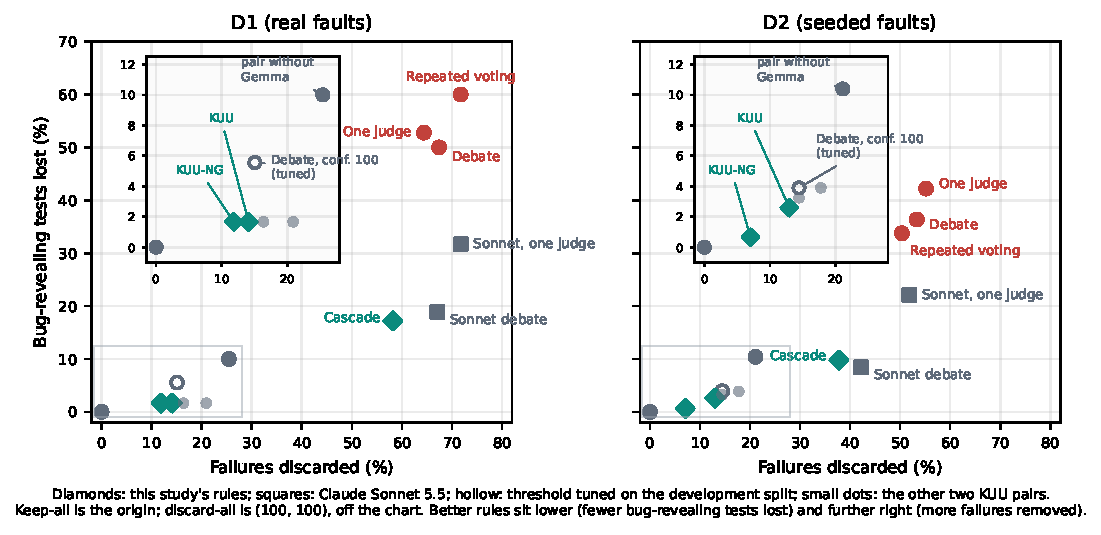
\includegraphics[width=0.8\textwidth]{figures/fig_pareto.pdf}
\caption{Share of failures each rule discards against the share of bug-revealing tests it loses (post hoc, descriptive). Insets enlarge the low-loss corner. Diamonds: this study's rules; squares: the frontier judge; the hollow point is the only rule with a threshold tuned on the development split.}\label{fig:tradeoff}
\end{figure*}

\par\medskip\noindent\begin{minipage}{\columnwidth}{\footnotesize\refstepcounter{table}\label{tab:rates}\textbf{Table~\thetable}\enspace Rates on a common scale (D-113), D-110's instance sets (D1-test \V{rv11:D1:n_instances}, D2 \V{rv11:D2:n_instances}). BA: balanced accuracy. FA: test faults kept per bug-revealing test kept at an assumed \PF{} prevalence of 5\%.\par}\smallskip
{\noindent\scriptsize\setlength{\tabcolsep}{2.5pt}
\resizebox{\columnwidth}{!}{\begin{tabular}{@{}l r r r r r r r@{}}
\toprule
 & \multicolumn{3}{c}{D1-test} & \multicolumn{3}{c}{D2} & \\
\cmidrule(lr){2-4}\cmidrule(lr){5-7}
Rule & TPR & TNR & BA & TPR & TNR & BA & FA$_{5\%}$ \\
\midrule
Keep-all & \V{rv11:D1:rules:KA:tpr} & \V{rv11:D1:rules:KA:tnr} & \V{rv11:D1:rules:KA:ba} & \V{rv11:D2:rules:KA:tpr} & \V{rv11:D2:rules:KA:tnr} & \V{rv11:D2:rules:KA:ba} & \V{rv11:D2:rules:KA:at_prevalence:0.0500:false_alarms_per_kept_pf@1} \\
R0 & \V{rv11:D1:rules:R0:tpr} & \V{rv11:D1:rules:R0:tnr} & \V{rv11:D1:rules:R0:ba} & \V{rv11:D2:rules:R0:tpr} & \V{rv11:D2:rules:R0:tnr} & \V{rv11:D2:rules:R0:ba} & \V{rv11:D2:rules:R0:at_prevalence:0.0500:false_alarms_per_kept_pf@1} \\
M1 J1 & \V{rv11:D1:rules:J1|S1:tpr} & \V{rv11:D1:rules:J1|S1:tnr} & \V{rv11:D1:rules:J1|S1:ba} & \V{rv11:D2:rules:J1|S1:tpr} & \V{rv11:D2:rules:J1|S1:tnr} & \V{rv11:D2:rules:J1|S1:ba} & \V{rv11:D2:rules:J1|S1:at_prevalence:0.0500:false_alarms_per_kept_pf@1} \\
M1 SC & \V{rv11:D1:rules:SC|S1:tpr} & \V{rv11:D1:rules:SC|S1:tnr} & \V{rv11:D1:rules:SC|S1:ba} & \V{rv11:D2:rules:SC|S1:tpr} & \V{rv11:D2:rules:SC|S1:tnr} & \V{rv11:D2:rules:SC|S1:ba} & \V{rv11:D2:rules:SC|S1:at_prevalence:0.0500:false_alarms_per_kept_pf@1} \\
M1 DEB & \V{rv11:D1:rules:DEB|S1:tpr} & \V{rv11:D1:rules:DEB|S1:tnr} & \V{rv11:D1:rules:DEB|S1:ba} & \V{rv11:D2:rules:DEB|S1:tpr} & \V{rv11:D2:rules:DEB|S1:tnr} & \V{rv11:D2:rules:DEB|S1:ba} & \V{rv11:D2:rules:DEB|S1:at_prevalence:0.0500:false_alarms_per_kept_pf@1} \\
M1 DEB, confidence 100 (tuned) & \V{rv11:D1:rules:TAU|S1:tpr} & \V{rv11:D1:rules:TAU|S1:tnr} & \V{rv11:D1:rules:TAU|S1:ba} & \V{rv11:D2:rules:TAU|S1:tpr} & \V{rv11:D2:rules:TAU|S1:tnr} & \V{rv11:D2:rules:TAU|S1:ba} & \V{rv11:D2:rules:TAU|S1:at_prevalence:0.0500:false_alarms_per_kept_pf@1} \\
Cross-family 2-of-3 & \V{rv11:D1:rules:MAJ3|S1:tpr} & \V{rv11:D1:rules:MAJ3|S1:tnr} & \V{rv11:D1:rules:MAJ3|S1:ba} & \V{rv11:D2:rules:MAJ3|S1:tpr} & \V{rv11:D2:rules:MAJ3|S1:tnr} & \V{rv11:D2:rules:MAJ3|S1:ba} & \V{rv11:D2:rules:MAJ3|S1:at_prevalence:0.0500:false_alarms_per_kept_pf@1} \\
KUU & \V{rv11:D1:rules:KUU|S1:tpr} & \V{rv11:D1:rules:KUU|S1:tnr} & \V{rv11:D1:rules:KUU|S1:ba} & \V{rv11:D2:rules:KUU|S1:tpr} & \V{rv11:D2:rules:KUU|S1:tnr} & \V{rv11:D2:rules:KUU|S1:ba} & \V{rv11:D2:rules:KUU|S1:at_prevalence:0.0500:false_alarms_per_kept_pf@1} \\
KUU-NG & \V{rv11:D1:rules:KUUNG|S1:tpr} & \V{rv11:D1:rules:KUUNG|S1:tnr} & \V{rv11:D1:rules:KUUNG|S1:ba} & \V{rv11:D2:rules:KUUNG|S1:tpr} & \V{rv11:D2:rules:KUUNG|S1:tnr} & \V{rv11:D2:rules:KUUNG|S1:ba} & \V{rv11:D2:rules:KUUNG|S1:at_prevalence:0.0500:false_alarms_per_kept_pf@1} \\
Cascade & \V{rv11:D1:rules:CAS|S1:tpr} & \V{rv11:D1:rules:CAS|S1:tnr} & \V{rv11:D1:rules:CAS|S1:ba} & \V{rv11:D2:rules:CAS|S1:tpr} & \V{rv11:D2:rules:CAS|S1:tnr} & \V{rv11:D2:rules:CAS|S1:ba} & \V{rv11:D2:rules:CAS|S1:at_prevalence:0.0500:false_alarms_per_kept_pf@1} \\
Sonnet J1 & \V{rv11:D1:rules:J1|S1|SON:tpr} & \V{rv11:D1:rules:J1|S1|SON:tnr} & \V{rv11:D1:rules:J1|S1|SON:ba} & \V{rv11:D2:rules:J1|S1|SON:tpr} & \V{rv11:D2:rules:J1|S1|SON:tnr} & \V{rv11:D2:rules:J1|S1|SON:ba} & \V{rv11:D2:rules:J1|S1|SON:at_prevalence:0.0500:false_alarms_per_kept_pf@1} \\
Sonnet DEB & \V{rv11:D1:rules:DEB|S1|SON:tpr} & \V{rv11:D1:rules:DEB|S1|SON:tnr} & \V{rv11:D1:rules:DEB|S1|SON:ba} & \V{rv11:D2:rules:DEB|S1|SON:tpr} & \V{rv11:D2:rules:DEB|S1|SON:tnr} & \V{rv11:D2:rules:DEB|S1|SON:ba} & \V{rv11:D2:rules:DEB|S1|SON:at_prevalence:0.0500:false_alarms_per_kept_pf@1} \\
\bottomrule
\end{tabular}}
\par}\end{minipage}\par\medskip

\noindent\textit{Reading.} KUU keeps almost every bug-revealing test but removes only a minority of test faults, so its balanced accuracy on D2 (\V{rv11:D2:rules:KUU|S1:ba}, 95\% CI \V{rv11:D2:rules:KUU|S1:ba_ci95}) is below M1 DEB's (\V{rv11:D2:rules:DEB|S1:ba}, \V{rv11:D2:rules:DEB|S1:ba_ci95}) and far below the cascade's (\V{rv11:D2:rules:CAS|S1:ba}, \V{rv11:D2:rules:CAS|S1:ba_ci95}). On D2, KUU-NG discards \V{rv11:reviewer_figures:kuung_share_discarded_D2@pct1} of failures, KUU \V{rv11:reviewer_figures:kuu_share_discarded_D2@pct1} and the cascade \V{rv11:reviewer_figures:cascade_share_discarded_D2@pct1}. At the D1-test labelled prevalence (\V{rv11:D1:population_pf_prevalence@3}) KUU keeps \V{rv11:D1:rules:KUU|S1:at_prevalence:0.1685:false_alarms_per_kept_pf@1} test faults per bug-revealing test kept, keep-all \V{rv11:D1:rules:KA:at_prevalence:0.1685:false_alarms_per_kept_pf@1}. Scoring invalid outputs as keep instead of \TF{} changes no single-judge arm's balanced accuracy by more than \V{der:inv keep max dBA@3}. Sonnet's DEB balanced accuracy on D1 minus D2 is \V{rv11:sonnet_e9_vs_e9b:DEB|S1|SON:ba:d1_minus_d2} (\V{rv11:sonnet_e9_vs_e9b:DEB|S1|SON:ba:d1_minus_d2_ci95}; unpaired, different instances and fault process, not a method effect).

\par\medskip\noindent\begin{minipage}{\columnwidth}{\footnotesize\refstepcounter{table}\label{tab:ranking}\textbf{Table~\thetable}\enspace Triage as ranking (D-114). Scores: stated confidence in the stated label for J1 and DEB, \PF{} vote share for SC, the number of non-\TF{} votes for the panels. Top 20\%: share of \PF{} tests (test) and of bugs with a \PF{} test (bug) found in the highest-scored 20\% of failures; random inspection finds 20\% of tests.\par}\smallskip
{\noindent\scriptsize\setlength{\tabcolsep}{2.5pt}
\resizebox{\columnwidth}{!}{\begin{tabular}{@{}l l l r r r r@{}}
\toprule
 & \multicolumn{2}{c}{AUROC [95\% CI]} & \multicolumn{2}{c}{D1 top 20\%} & \multicolumn{2}{c}{D2 top 20\%} \\
\cmidrule(lr){2-3}\cmidrule(lr){4-5}\cmidrule(lr){6-7}
Score & D1-test & D2 & test & bug & test & bug \\
\midrule
Keep-all & \V{rv13:D1:rules:KA:auroc} & \V{rv13:D2:rules:KA:auroc} & \V{rv13:D1:rules:KA:inspection:top20:recall@2} & \V{rv13:D1:rules:KA:inspection:top20:bug_recall@2} & \V{rv13:D2:rules:KA:inspection:top20:recall@2} & \V{rv13:D2:rules:KA:inspection:top20:bug_recall@2} \\
M1 J1 & \V{rv13:D1:rules:J1|S1:auroc} \V{rv13:D1:rules:J1|S1:auroc_ci95} & \V{rv13:D2:rules:J1|S1:auroc} \V{rv13:D2:rules:J1|S1:auroc_ci95} & \V{rv13:D1:rules:J1|S1:inspection:top20:recall@2} & \V{rv13:D1:rules:J1|S1:inspection:top20:bug_recall@2} & \V{rv13:D2:rules:J1|S1:inspection:top20:recall@2} & \V{rv13:D2:rules:J1|S1:inspection:top20:bug_recall@2} \\
M1 SC & \V{rv13:D1:rules:SC|S1:auroc} \V{rv13:D1:rules:SC|S1:auroc_ci95} & \V{rv13:D2:rules:SC|S1:auroc} \V{rv13:D2:rules:SC|S1:auroc_ci95} & \V{rv13:D1:rules:SC|S1:inspection:top20:recall@2} & \V{rv13:D1:rules:SC|S1:inspection:top20:bug_recall@2} & \V{rv13:D2:rules:SC|S1:inspection:top20:recall@2} & \V{rv13:D2:rules:SC|S1:inspection:top20:bug_recall@2} \\
M1 DEB & \V{rv13:D1:rules:DEB|S1:auroc} \V{rv13:D1:rules:DEB|S1:auroc_ci95} & \V{rv13:D2:rules:DEB|S1:auroc} \V{rv13:D2:rules:DEB|S1:auroc_ci95} & \V{rv13:D1:rules:DEB|S1:inspection:top20:recall@2} & \V{rv13:D1:rules:DEB|S1:inspection:top20:bug_recall@2} & \V{rv13:D2:rules:DEB|S1:inspection:top20:recall@2} & \V{rv13:D2:rules:DEB|S1:inspection:top20:bug_recall@2} \\
KUU panel votes & \V{rv13:D1:rules:KUU|S1:auroc} \V{rv13:D1:rules:KUU|S1:auroc_ci95} & \V{rv13:D2:rules:KUU|S1:auroc} \V{rv13:D2:rules:KUU|S1:auroc_ci95} & \V{rv13:D1:rules:KUU|S1:inspection:top20:recall@2} & \V{rv13:D1:rules:KUU|S1:inspection:top20:bug_recall@2} & \V{rv13:D2:rules:KUU|S1:inspection:top20:recall@2} & \V{rv13:D2:rules:KUU|S1:inspection:top20:bug_recall@2} \\
KUU-NG panel votes & \V{rv13:D1:rules:KUUNG|S1:auroc} \V{rv13:D1:rules:KUUNG|S1:auroc_ci95} & \V{rv13:D2:rules:KUUNG|S1:auroc} \V{rv13:D2:rules:KUUNG|S1:auroc_ci95} & \V{rv13:D1:rules:KUUNG|S1:inspection:top20:recall@2} & \V{rv13:D1:rules:KUUNG|S1:inspection:top20:bug_recall@2} & \V{rv13:D2:rules:KUUNG|S1:inspection:top20:recall@2} & \V{rv13:D2:rules:KUUNG|S1:inspection:top20:bug_recall@2} \\
Sonnet DEB & \V{rv13:D1:rules:DEB|S1|SON:auroc} \V{rv13:D1:rules:DEB|S1|SON:auroc_ci95} & \V{rv13:D2:rules:DEB|S1|SON:auroc} \V{rv13:D2:rules:DEB|S1|SON:auroc_ci95} & \V{rv13:D1:rules:DEB|S1|SON:inspection:top20:recall@2} & \V{rv13:D1:rules:DEB|S1|SON:inspection:top20:bug_recall@2} & \V{rv13:D2:rules:DEB|S1|SON:inspection:top20:recall@2} & \V{rv13:D2:rules:DEB|S1|SON:inspection:top20:bug_recall@2} \\
\bottomrule
\end{tabular}}
\par}\end{minipage}\par\medskip

\noindent\textit{Reading.} Confidence adds to the label for every judge (M1 DEB AUROC \V{rv13:D1:rules:DEB|S1:auroc} with confidence, \V{rv13:D1:rules:DEB|S1:auroc_label_only} from the label alone, D1). Test-level and bug-level recall need not agree: on D2 Sonnet's top 20\% are all \PF{} tests (precision \V{rv13:D2:rules:DEB|S1|SON:inspection:top20:precision@2}), yet they cover fewer bugs (\V{rv13:D2:rules:DEB|S1|SON:inspection:top20:bug_recall@2}) than random inspection (\V{rv13:D2:rules:KA:inspection:top20:bug_recall@2}), because its most confident \PF{} tests cluster in a few bugs. Reweighted to the D1-test labelled population (\PF{} share \V{rv13:D1:reweighting:weighted_pf_share@3}), the KUU panel's AUPRC is \V{rv13:D1:rules:KUU|S1:reweighted:auprc} against \V{rv13:D1:rules:KUU|S1:reweighted:auprc_random} for a random order and Sonnet DEB's \V{rv13:D1:rules:DEB|S1|SON:reweighted:auprc}; the reweighting assumes the sampled test faults represent their project's.

\par\medskip\noindent\begin{minipage}{\columnwidth}{\footnotesize\refstepcounter{table}\label{tab:learned}\textbf{Table~\thetable}\enspace Trained baselines (D-115, exploratory): logistic regression, leave-one-project-out on D1-test (pooled out-of-fold predictions, threshold 0.5 fixed in advance, nothing tuned), and one transfer to D2. Failure features: assertion or exception, exception family, deepest project frame, expected/actual values present. Votes: the KUU members' J1 votes.\par}\smallskip
{\noindent\scriptsize\setlength{\tabcolsep}{2.5pt}
\resizebox{\columnwidth}{!}{\begin{tabular}{@{}l r r l l r r@{}}
\toprule
 & \multicolumn{4}{c}{D1-test, leave one project out} & \multicolumn{2}{c}{D1 $\to$ D2} \\
\cmidrule(lr){2-5}\cmidrule(lr){6-7}
Model & TPR & TNR & BA [95\% CI] & AUROC [95\% CI] & BA & AUROC \\
\midrule
Failure features only (no LLM) & \V{rv14:lopo:features:tpr} & \V{rv14:lopo:features:tnr} & \V{rv14:lopo:features:ba} \V{rv14:lopo:features:ba_ci95} & \V{rv14:lopo:features:auroc} \V{rv14:lopo:features:auroc_ci95} & \V{rv14:transfer_D1_to_D2:features:ba} & \V{rv14:transfer_D1_to_D2:features:auroc} \\
Votes only & \V{rv14:lopo:votes:tpr} & \V{rv14:lopo:votes:tnr} & \V{rv14:lopo:votes:ba} \V{rv14:lopo:votes:ba_ci95} & \V{rv14:lopo:votes:auroc} \V{rv14:lopo:votes:auroc_ci95} & \V{rv14:transfer_D1_to_D2:votes:ba} & \V{rv14:transfer_D1_to_D2:votes:auroc} \\
Stacker (votes + features) & \V{rv14:lopo:stacker:tpr} & \V{rv14:lopo:stacker:tnr} & \V{rv14:lopo:stacker:ba} \V{rv14:lopo:stacker:ba_ci95} & \V{rv14:lopo:stacker:auroc} \V{rv14:lopo:stacker:auroc_ci95} & \V{rv14:transfer_D1_to_D2:stacker:ba} & \V{rv14:transfer_D1_to_D2:stacker:auroc} \\
Stacker + cross-generation & \V{rv14:lopo:stacker+cg:tpr} & \V{rv14:lopo:stacker+cg:tnr} & \V{rv14:lopo:stacker+cg:ba} \V{rv14:lopo:stacker+cg:ba_ci95} & \V{rv14:lopo:stacker+cg:auroc} \V{rv14:lopo:stacker+cg:auroc_ci95} & \V{rv14:transfer_D1_to_D2:stacker+cg:ba} & \V{rv14:transfer_D1_to_D2:stacker+cg:auroc} \\
KUU (no training) & \V{rv11:D1:rules:KUU|S1:tpr} & \V{rv11:D1:rules:KUU|S1:tnr} & \V{rv11:D1:rules:KUU|S1:ba} \V{rv11:D1:rules:KUU|S1:ba_ci95} & \V{rv13:D1:rules:KUU|S1:auroc} \V{rv13:D1:rules:KUU|S1:auroc_ci95} & \V{rv11:D2:rules:KUU|S1:ba} & \V{rv13:D2:rules:KUU|S1:auroc} \\
\bottomrule
\end{tabular}}
\par}\end{minipage}\par\medskip

\noindent\textit{Reading.} The failure features alone carry little signal across projects; a learned weighting of the three votes reaches a higher balanced accuracy than KUU but keeps fewer bug-revealing tests (TPR \V{rv14:lopo:votes:tpr} against \V{rv11:D1:rules:KUU|S1:tpr}), the trade-off a threshold moves along; the failure features and the cross-generation signal add nothing to the votes.

\par\medskip\noindent\begin{minipage}{\columnwidth}{\footnotesize\refstepcounter{table}\label{tab:kofn}\textbf{Table~\thetable}\enspace Discard when at least $k$ of three judges vote \TF{} (D-116): \PF{}-loss rate (1 $-$ TPR) / \TF{}-removal rate (TNR). $k=3$ of the KUU panel is KUU. Within-model: the first three of five SC samples.\par}\smallskip
{\noindent\scriptsize\setlength{\tabcolsep}{2.5pt}
\resizebox{\columnwidth}{!}{\begin{tabular}{@{}l l l l l l l@{}}
\toprule
 & \multicolumn{3}{c}{D1-test} & \multicolumn{3}{c}{D2} \\
\cmidrule(lr){2-4}\cmidrule(lr){5-7}
Triple & $k=1$ & $k=2$ & $k=3$ & $k=1$ & $k=2$ & $k=3$ \\
\midrule
KUU panel & \V{rv15:D1:triples:KUUpanel(M1,M2,E6b):k=1:pf_loss_rate@2}/\V{rv15:D1:triples:KUUpanel(M1,M2,E6b):k=1:tnr@2} & \V{rv15:D1:triples:KUUpanel(M1,M2,E6b):k=2:pf_loss_rate@2}/\V{rv15:D1:triples:KUUpanel(M1,M2,E6b):k=2:tnr@2} & \V{rv15:D1:triples:KUUpanel(M1,M2,E6b):k=3:pf_loss_rate@2}/\V{rv15:D1:triples:KUUpanel(M1,M2,E6b):k=3:tnr@2} & \V{rv15:D2:triples:KUUpanel(M1,M2,E6b):k=1:pf_loss_rate@2}/\V{rv15:D2:triples:KUUpanel(M1,M2,E6b):k=1:tnr@2} & \V{rv15:D2:triples:KUUpanel(M1,M2,E6b):k=2:pf_loss_rate@2}/\V{rv15:D2:triples:KUUpanel(M1,M2,E6b):k=2:tnr@2} & \V{rv15:D2:triples:KUUpanel(M1,M2,E6b):k=3:pf_loss_rate@2}/\V{rv15:D2:triples:KUUpanel(M1,M2,E6b):k=3:tnr@2} \\
KUU-NG panel & \V{rv15:D1:triples:KUU-NGpanel(M1,E6b,Llama):k=1:pf_loss_rate@2}/\V{rv15:D1:triples:KUU-NGpanel(M1,E6b,Llama):k=1:tnr@2} & \V{rv15:D1:triples:KUU-NGpanel(M1,E6b,Llama):k=2:pf_loss_rate@2}/\V{rv15:D1:triples:KUU-NGpanel(M1,E6b,Llama):k=2:tnr@2} & \V{rv15:D1:triples:KUU-NGpanel(M1,E6b,Llama):k=3:pf_loss_rate@2}/\V{rv15:D1:triples:KUU-NGpanel(M1,E6b,Llama):k=3:tnr@2} & \V{rv15:D2:triples:KUU-NGpanel(M1,E6b,Llama):k=1:pf_loss_rate@2}/\V{rv15:D2:triples:KUU-NGpanel(M1,E6b,Llama):k=1:tnr@2} & \V{rv15:D2:triples:KUU-NGpanel(M1,E6b,Llama):k=2:pf_loss_rate@2}/\V{rv15:D2:triples:KUU-NGpanel(M1,E6b,Llama):k=2:tnr@2} & \V{rv15:D2:triples:KUU-NGpanel(M1,E6b,Llama):k=3:pf_loss_rate@2}/\V{rv15:D2:triples:KUU-NGpanel(M1,E6b,Llama):k=3:tnr@2} \\
M1 within-model & \V{rv15:D1:triples:M1within-model(first3SCsamples):k=1:pf_loss_rate@2}/\V{rv15:D1:triples:M1within-model(first3SCsamples):k=1:tnr@2} & \V{rv15:D1:triples:M1within-model(first3SCsamples):k=2:pf_loss_rate@2}/\V{rv15:D1:triples:M1within-model(first3SCsamples):k=2:tnr@2} & \V{rv15:D1:triples:M1within-model(first3SCsamples):k=3:pf_loss_rate@2}/\V{rv15:D1:triples:M1within-model(first3SCsamples):k=3:tnr@2} & \V{rv15:D2:triples:M1within-model(first3SCsamples):k=1:pf_loss_rate@2}/\V{rv15:D2:triples:M1within-model(first3SCsamples):k=1:tnr@2} & \V{rv15:D2:triples:M1within-model(first3SCsamples):k=2:pf_loss_rate@2}/\V{rv15:D2:triples:M1within-model(first3SCsamples):k=2:tnr@2} & \V{rv15:D2:triples:M1within-model(first3SCsamples):k=3:pf_loss_rate@2}/\V{rv15:D2:triples:M1within-model(first3SCsamples):k=3:tnr@2} \\
M2 within-model & \V{rv15:D1:triples:M2within-model(first3SCsamples):k=1:pf_loss_rate@2}/\V{rv15:D1:triples:M2within-model(first3SCsamples):k=1:tnr@2} & \V{rv15:D1:triples:M2within-model(first3SCsamples):k=2:pf_loss_rate@2}/\V{rv15:D1:triples:M2within-model(first3SCsamples):k=2:tnr@2} & \V{rv15:D1:triples:M2within-model(first3SCsamples):k=3:pf_loss_rate@2}/\V{rv15:D1:triples:M2within-model(first3SCsamples):k=3:tnr@2} & \V{rv15:D2:triples:M2within-model(first3SCsamples):k=1:pf_loss_rate@2}/\V{rv15:D2:triples:M2within-model(first3SCsamples):k=1:tnr@2} & \V{rv15:D2:triples:M2within-model(first3SCsamples):k=2:pf_loss_rate@2}/\V{rv15:D2:triples:M2within-model(first3SCsamples):k=2:tnr@2} & \V{rv15:D2:triples:M2within-model(first3SCsamples):k=3:pf_loss_rate@2}/\V{rv15:D2:triples:M2within-model(first3SCsamples):k=3:tnr@2} \\
\bottomrule
\end{tabular}}
\par}\end{minipage}\par\medskip

\par\medskip\noindent\begin{minipage}{\columnwidth}{\footnotesize\refstepcounter{table}\label{tab:revmisc}\textbf{Table~\thetable}\enspace Risk-targeted threshold (D-117), cross-generation signal (D-118), sample-size planning (D-119), integrity checks (D-120), the leakage guard's selection (D-121) and label-noise sensitivity (D-121).\par}\smallskip
{\noindent\scriptsize\setlength{\tabcolsep}{3pt}
\resizebox{\columnwidth}{!}{\begin{tabular}{@{}l r@{}}
\toprule
Quantity & Value \\
\midrule
\multicolumn{2}{@{}l}{\textit{Risk-targeted threshold, $\alpha=0.05$ on \PF{} tests, calibrated on D1, evaluated on D2 (a heuristic: see text)}} \\
KUU panel + DEB confidence: D2 \PF{}-loss / \TF{}-removal & \V{rv16:panels:KUU:thresholds:tests_alpha0.05:D2_evaluation:pf_loss_rate} / \V{rv16:panels:KUU:thresholds:tests_alpha0.05:D2_evaluation:tnr} \\
KUU-NG panel + DEB confidence: D2 \PF{}-loss / \TF{}-removal & \V{rv16:panels:KUU-NG:thresholds:tests_alpha0.05:D2_evaluation:pf_loss_rate} / \V{rv16:panels:KUU-NG:thresholds:tests_alpha0.05:D2_evaluation:tnr} \\
\multicolumn{2}{@{}l}{\textit{Cross-generation agreement (buggy version only): AUROC}} \\
D1-test / D2 & \V{rv17:D1:auroc_cg} \V{rv17:D1:auroc_cg_ci95} / \V{rv17:D2:auroc_cg} \V{rv17:D2:auroc_cg_ci95} \\
\multicolumn{2}{@{}l}{\textit{Bugs needed for an MDE of 0.08 (0.05) at 80\% power, $\alpha=0.05$; now \V{rv18:tests:H3a:n0_bugs} bugs}} \\
H3a (DEB vs SC) & \V{rv18:tests:H3a:by_mde:0.08:bugs_alpha_005} (\V{rv18:tests:H3a:by_mde:0.05:bugs_alpha_005}), \V{rv18:tests:H3a:by_mde:0.08:multiplier_alpha_005@1}$\times$ \\
H2a (Javadoc) & \V{rv18:tests:H2a:by_mde:0.08:bugs_alpha_005} (\V{rv18:tests:H2a:by_mde:0.05:bugs_alpha_005}) \\
\multicolumn{2}{@{}l}{\textit{Integrity}} \\
Holm families reproduced from stored $p$ & \V{der:holm all match} \V{der:holm families} \\
\multicolumn{2}{@{}l}{\textit{Leakage-guard aborts among judged D2 instances}} \\
Aborted (\PF{}, matched the injected line) & \V{rv110:guard:D2:aborted_at_S1_any_run} of \V{rv110:guard:D2:judged} (\V{rv110:guard:D2:aborted_by_label:PF}, \V{rv110:guard:D2:aborted_matched_kind:themutatedline}) \\
Scored \PF{} prevalence with / without aborts & \V{rv110:guard:D2:judged_with_aborts:pf_prevalence_scored} / \V{rv110:guard:D2:judged_without_aborts:pf_prevalence_scored} \\
\multicolumn{2}{@{}l}{\textit{Label noise: execution-\TF{} assertion failures relabelled \PF{} (median BA over 1{,}000 draws)}} \\
D2 KUU: none / audit rate \V{rv110:noise_model:audit_rate:value@2} / 0.10 & \V{rv110:noise:D2:no_noise:KUU|S1:ba} / \V{rv110:noise:D2:rules:q=0.0400:KUU|S1:ba:median} / \V{rv110:noise:D2:rules:q=0.1000:KUU|S1:ba:median} \\
D1 Sonnet DEB: none / audit rate / 0.10 & \V{rv110:noise:D1:no_noise:DEB|S1|SON:ba} / \V{rv110:noise:D1:rules:q=0.0400:DEB|S1|SON:ba:median} / \V{rv110:noise:D1:rules:q=0.1000:DEB|S1|SON:ba:median} \\
\bottomrule
\end{tabular}}
\par}\end{minipage}\par\medskip

\noindent\textit{Reading.} The risk-targeted threshold is not a conformal guarantee: its calibration set (D1) is the data KUU was designed on and is not exchangeable with D2 (different fault process and prevalence). The two panels show why this matters: calibrated to the same target, one stays within it on D2 and the other does not. Cross-generation agreement is a signal for seeded faults but not for real ones. The planning numbers assume the bootstrap standard error falls as one over the square root of the number of bugs; they are guidance, not a power guarantee. Every interval in the paper resamples bugs (the label-audit $\kappa$ uses 2{,}000 resamples, as fixed in D-82). The guard removed the D2 instances whose evidence showed the injected line, so the scored D2 set under-represents faults visible in the test evidence. The label-noise model is hypothetical (the audit rate comes from development-split items rated by the authors); it moves no rule's balanced accuracy enough to change the order of the rules.

\par\medskip\noindent\begin{minipage}{\columnwidth}{\footnotesize\refstepcounter{table}\label{tab:gates}\textbf{Table~\thetable}\enspace Development gates of every local judge (dev pilot, \V{devgate:n_instances} instances): G-a output validity, G-b evidence citation, G-c, G-d one-shot F1 above both trivial baselines (R0: \V{rv2:gates:M1(Qwen3.59B):R0_f1_dev}). Sonnet and the 35B judge were not gated.\par}\smallskip
{\noindent\scriptsize\setlength{\tabcolsep}{4pt}
\resizebox{\columnwidth}{!}{\begin{tabular}{@{}l c c c c r@{}}
\toprule
Judge & G-a & G-b & G-c & G-d & J1 F1 (dev) \\
\midrule
M1 Qwen3.5 9B & \V{der:gate M1 G_a} & \V{der:gate M1 G_b} & \V{der:gate M1 G_c} & \V{der:gate M1 G_d} & \V{rv2:gates:M1(Qwen3.59B):J1_f1_dev} \\
M2 Gemma~4 12B & \V{der:gate M2 G_a} & \V{der:gate M2 G_b} & \V{der:gate M2 G_c} & \V{der:gate M2 G_d} & \V{rv2:gates:M2(Gemma412B):J1_f1_dev} \\
M3 Ministral~3 14B & \V{der:gate M3 G_a} & \V{der:gate M3 G_b} & \V{der:gate M3 G_c} & \V{der:gate M3 G_d} & \V{rv2:gates:E6b(Ministral314B):J1_f1_dev} \\
NG Llama~3.1 8B & \V{der:gate NG G_a} & \V{der:gate NG G_b} & \V{der:gate NG G_c} & \V{der:gate NG G_d} & \V{rv2:gates:NG(Llama3.18B):J1_f1_dev} \\
\bottomrule
\end{tabular}}
\par}\end{minipage}\par\medskip

\par\medskip\noindent\begin{minipage}{\columnwidth}{\footnotesize\refstepcounter{table}\label{tab:wp2}\textbf{Table~\thetable}\enspace Local runs added in response to review (D-123 to D-127, exploratory; own server, frozen prompts, the D-109 stopping rule). (a) The \V{der:tf176 n} D1-test test faults the 1:2 sample left out, judged by M1, M2, M3 and NG and pooled with the sampled ones; precision and false alarms are at the natural prevalence, with no weights. (b) M1's one-shot judge at temperature 0. (c) M1's one-shot judge with thinking enabled (context \V{cfgth:spec_patch:num_ctx@int} tokens, output cap \V{cfgth:max_tokens@int}, thinking included); Ollama caps total output, not thinking, so the run is not token-matched by construction. (d) M1 DEB, eight replicates (three committed, five new).\par}\smallskip
{\noindent\scriptsize\setlength{\tabcolsep}{3pt}
\resizebox{\columnwidth}{!}{\begin{tabular}{@{}l r@{}}
\toprule
Quantity & Value \\
\midrule
\multicolumn{2}{@{}l}{\textit{(a) All judgeable D1-test test faults: \V{rv2:tf296:n_tf_judged} of \V{der:d1 test TF labelled}, with the \V{rv2:tf296:n_pf} \PF{}}} \\
KUU: TNR all [95\% CI]; sampled / new & \V{rv2:tf296:rules:KUU:all:tnr} \V{rv2:tf296:rules:KUU:all:tnr_ci95}; \V{rv2:tf296:rules:KUU:tnr_original_sample} / \V{rv2:tf296:rules:KUU:tnr_new_176} \\
KUU-NG: TNR all; sampled / new & \V{rv2:tf296:rules:KUU-NG:all:tnr} \V{rv2:tf296:rules:KUU-NG:all:tnr_ci95}; \V{rv2:tf296:rules:KUU-NG:tnr_original_sample} / \V{rv2:tf296:rules:KUU-NG:tnr_new_176} \\
M1 J1: TNR all; sampled / new & \V{rv2:tf296:rules:M1J1:all:tnr} \V{rv2:tf296:rules:M1J1:all:tnr_ci95}; \V{rv2:tf296:rules:M1J1:tnr_original_sample} / \V{rv2:tf296:rules:M1J1:tnr_new_176} \\
Precision: keep-all / KUU / KUU-NG / M1 J1 & \V{rv2:tf296:rules:Keepall:all:precision} / \V{rv2:tf296:rules:KUU:all:precision} / \V{rv2:tf296:rules:KUU-NG:all:precision} / \V{rv2:tf296:rules:M1J1:all:precision} \\
Test faults per kept \PF{} test: keep-all / KUU / KUU-NG & \V{rv2:tf296:rules:Keepall:all:false_alarms_per_kept_pf@1} / \V{rv2:tf296:rules:KUU:all:false_alarms_per_kept_pf@1} / \V{rv2:tf296:rules:KUU-NG:all:false_alarms_per_kept_pf@1} \\
\multicolumn{2}{@{}l}{\textit{(b) Greedy one-shot judge, D1-test (\V{rv11:D1:n_instances} instances)}} \\
BA / F1 / MCC at temperature \V{cfgt0:temperature@1} & \V{rv2:greedy:temperature_0:50:ba} / \V{rv2:greedy:temperature_0:50:f1} / \V{rv2:greedy:temperature_0:50:mcc} \\
BA / F1 / MCC at \V{frozen:frozen_models:M1:temperature:judges@1} (three replicates) & \V{rv11:D1:rules:J1|S1:ba} / \V{rv11:D1:rules:J1|S1:f1} / \V{rv11:D1:rules:J1|S1:mcc} \\
\multicolumn{2}{@{}l}{\textit{(c) Thinking-enabled one-shot judge (M1, one run), D1-test (\V{rv2:think:heldout:60:n} instances)}} \\
BA / F1 / MCC & \V{rv2:think:heldout:60:ba} / \V{rv2:think:heldout:60:f1} / \V{rv2:think:heldout:60:mcc} \\
TPR / TNR; \PF{} tests lost; no answer (output cap) & \V{rv2:think:heldout:60:tpr} / \V{rv2:think:heldout:60:tnr}; \V{rv2:think:heldout:60:FN@0}; \V{rv2:think:heldout:60:invalid@0} \\
Consumed tokens per instance (M1 DEB \V{rv2:think:deb_consumed_tokens_per_instance_table@0}) & \V{rv2:think:heldout:60:consumed_tokens_per_instance@0} (\V{rv2:think:heldout:60:ratio_to_deb_tokens@2}$\times$; not token-matched) \\
BA of M1 DEB / SC-T (three runs, mean) & \V{rv11:D1:rules:DEB|S1:ba} / \V{rv11:D1:rules:SC-T|S1:ba} \\
\multicolumn{2}{@{}l}{\textit{(d) Debate replicates: \V{rv2:deb8:n_replicates} runs of M1 DEB on D1-test}} \\
F1 min--max (range, SD) & \V{rv2:deb8:spread:f1:min}--\V{rv2:deb8:spread:f1:max} (\V{rv2:deb8:spread:f1:range}, \V{rv2:deb8:spread:f1:sd}) \\
BA min--max (range) & \V{rv2:deb8:spread:ba:min}--\V{rv2:deb8:spread:ba:max} (\V{rv2:deb8:spread:ba:range}) \\
MCC min--max & \V{rv2:deb8:spread:mcc:min}--\V{rv2:deb8:spread:mcc:max} \\
\bottomrule
\end{tabular}}
\par}\end{minipage}\par\medskip

\par\medskip\noindent\begin{minipage}{\columnwidth}{\footnotesize\refstepcounter{table}\label{tab:think}\textbf{Table~\thetable}\enspace Thinking-enabled M1 one-shot judge, followed up as KUU was (D-130). Same configuration in every run (Table~\ref{tab:wp2}c); the development gate, the D2 hypotheses (one Holm family, paired bug-level bootstrap, 10{,}000 resamples) and the wording rule for this paper were fixed in advance in the version-controlled decision log. Primary coding: an output cut off by the cap scores \TF{}; the other codings are sensitivity only. Descriptive rows use D-110's common sets and are not tests. Tokens: Ollama prompt plus generated tokens, thinking included; not token-matched to debate.\par}\smallskip
{\noindent\scriptsize\setlength{\tabcolsep}{3pt}
\resizebox{\columnwidth}{!}{\begin{tabular}{@{}l r@{}}
\toprule
Quantity & Value \\
\midrule
\multicolumn{2}{@{}l}{\textit{(a) Development gate (dev pilot, \V{tk:gate:n_instances@int} labelled instances), as applied to M1}} \\
G-a valid outputs (needs $\geq$ 98\%) & \V{tk:gate:G_a_valid_rate:J1@pct1} (\V{tk:gate:G_a_runaway_D39:J1:invalid_length@int} cut off by the cap) \\
G-d J1 F1 vs best trivial rule (R0); thinking-disabled M1 & \V{tk:gate:G_d_detail:J1_f1} vs \V{tk:gate:G_d_detail:R0_f1}; \V{tk:gate:m1_original:J1_f1} \\
\multicolumn{2}{@{}l}{\textit{(b) D2 confirmation (\V{tk:d2:confirmatory:n_instances@int} instances, \V{tk:d2:confirmatory:n_bugs@int} bugs), thinking J1 vs M1 DEB}} \\
HT-1 $\Delta$MCC [95\% CI]; $p_\mathrm{Holm}$ & \V{tk:d2:confirmatory:HT-1:delta} \V{tk:d2:confirmatory:HT-1:ci95}; \V{tk:d2:confirmatory:HT-1:p_holm} \\
HT-2 $\Delta$\PF{} tests lost [95\% CI]; $p_\mathrm{Holm}$ & \V{tk:d2:confirmatory:HT-2:delta@int} \V{tk:d2:confirmatory:HT-2:ci95@ci0}; \V{tk:d2:confirmatory:HT-2:p_holm} \\
Cut off by the cap; HT-1 / HT-2 $\Delta$ if kept & \V{tk:d2:capped@int}; \V{tk:d2:policies:keep:hypotheses:HT-1:delta} / \V{tk:d2:policies:keep:hypotheses:HT-2:delta@int} \\
HT-1 / HT-2 $\Delta$ if excluded & \V{tk:d2:policies:exclude:hypotheses:HT-1:delta} / \V{tk:d2:policies:exclude:hypotheses:HT-2:delta@int} \\
\multicolumn{2}{@{}l}{\textit{(c) D2, descriptive: BA / TPR / TNR; \PF{} tests lost; bugs lost}} \\
Thinking M1 J1 & \V{tk:d2:descriptive:ThinkingM1J1:ba} / \V{tk:d2:descriptive:ThinkingM1J1:tpr} / \V{tk:d2:descriptive:ThinkingM1J1:tnr}; \V{tk:d2:descriptive:ThinkingM1J1:pf_lost@int}; \V{tk:d2:descriptive:ThinkingM1J1:bugs_lost@int} \\
M1 DEB & \V{tk:d2:descriptive:M1DEB:ba} / \V{tk:d2:descriptive:M1DEB:tpr} / \V{tk:d2:descriptive:M1DEB:tnr}; \V{tk:d2:descriptive:M1DEB:pf_lost@int}; \V{tk:d2:descriptive:M1DEB:bugs_lost@int} \\
KUU & \V{tk:d2:descriptive:KUU:ba} / \V{tk:d2:descriptive:KUU:tpr} / \V{tk:d2:descriptive:KUU:tnr}; \V{tk:d2:descriptive:KUU:pf_lost@int}; \V{tk:d2:descriptive:KUU:bugs_lost@int} \\
KUU-NG & \V{tk:d2:descriptive:KUU-NG:ba} / \V{tk:d2:descriptive:KUU-NG:tpr} / \V{tk:d2:descriptive:KUU-NG:tnr}; \V{tk:d2:descriptive:KUU-NG:pf_lost@int}; \V{tk:d2:descriptive:KUU-NG:bugs_lost@int} \\
Cascade & \V{tk:d2:descriptive:Cascade:ba} / \V{tk:d2:descriptive:Cascade:tpr} / \V{tk:d2:descriptive:Cascade:tnr}; \V{tk:d2:descriptive:Cascade:pf_lost@int}; \V{tk:d2:descriptive:Cascade:bugs_lost@int} \\
Sonnet DEB (frontier reference) & \V{tk:d2:descriptive:SonnetDEB:ba} / \V{tk:d2:descriptive:SonnetDEB:tpr} / \V{tk:d2:descriptive:SonnetDEB:tnr}; \V{tk:d2:descriptive:SonnetDEB:pf_lost@int}; \V{tk:d2:descriptive:SonnetDEB:bugs_lost@int} \\
\PF{} tests lost by thinking J1 but kept by KUU; the reverse & \V{tk:d2:kuu_vs_thinking:pf_lost_by_thinking_kept_by_kuu@int}; \V{tk:d2:kuu_vs_thinking:pf_lost_by_kuu_kept_by_thinking@int} \\
\multicolumn{2}{@{}l}{\textit{(d) D1-test, three runs (replicates 60, 63, 64; exploratory, found on these data)}} \\
BA per run & \V{tk:d1:runs:60:ba} / \V{tk:d1:runs:63:ba} / \V{tk:d1:runs:64:ba} \\
MCC per run & \V{tk:d1:runs:60:mcc} / \V{tk:d1:runs:63:mcc} / \V{tk:d1:runs:64:mcc} \\
F1 range (M1 DEB, eight runs) & \V{tk:d1:summary:f1:min}--\V{tk:d1:summary:f1:max} (\V{tk:d1:deb_eight_runs:f1:min}--\V{tk:d1:deb_eight_runs:f1:max}) \\
\PF{} tests lost per run (of \V{sum:prevalence:PF}); cut off by the cap & \V{tk:d1:runs:60:pf_lost@int} / \V{tk:d1:runs:63:pf_lost@int} / \V{tk:d1:runs:64:pf_lost@int}; \V{tk:d1:runs:60:capped@int} / \V{tk:d1:runs:63:capped@int} / \V{tk:d1:runs:64:capped@int} \\
Tokens per instance, D1 mean / D2 (M1 DEB on D1) & \V{tk:d1:summary:tokens_per_instance:mean@0} / \V{tk:d2:tokens_per_instance@0} (\V{tk:deb_tokens_per_instance_D1@0}) \\
\bottomrule
\end{tabular}}
\par}\end{minipage}\par\medskip

\par\medskip\noindent\begin{minipage}{\columnwidth}{\footnotesize\refstepcounter{table}\label{tab:localcas}\textbf{Table~\thetable}\enspace Fully local cascade (D-132, \emph{post hoc} on both sets, zero calls): KUU's unanimous votes decide; any disagreement goes to the logged thinking-enabled M1 J1 (Table~\ref{tab:think}), whose valid label decides, and an invalid or capped answer keeps the test. One rule, fixed in advance in the version-controlled decision log; no other variant was computed. Local minus Sonnet cascade on D2: $\Delta$BA \V{lc:D2:runs:62:local_minus_sonnet_cascade:ba:delta} \V{lc:D2:runs:62:local_minus_sonnet_cascade:ba:ci95}, $\Delta$MCC \V{lc:D2:runs:62:local_minus_sonnet_cascade:mcc:delta} \V{lc:D2:runs:62:local_minus_sonnet_cascade:mcc:ci95} (paired bug-level bootstrap, descriptive, no test). Lost: \PF{} tests lost; bugs: bugs with a \PF{} test and none kept; disc.: share of failures discarded. To be confirmed on fresh real faults (journal plan).\par}\smallskip
{\noindent\scriptsize\setlength{\tabcolsep}{2.5pt}
\resizebox{\columnwidth}{!}{\begin{tabular}{@{}l rrrrrrrr@{}}
\toprule
Rule & F1 & MCC & BA & TPR & TNR & Lost & Bugs & Disc. \\
\midrule
\multicolumn{9}{@{}l}{\textit{D2 (\V{lc:D2:n_instances@int} instances, \V{lc:D2:n_bugs@int} bugs; \V{lc:D2:share_escalated@pct0} reach Tier~2)}} \\
Fully local cascade & \V{lc:D2:runs:62:local_cascade:f1} & \V{lc:D2:runs:62:local_cascade:mcc} & \V{lc:D2:runs:62:local_cascade:ba} & \V{lc:D2:runs:62:local_cascade:tpr} & \V{lc:D2:runs:62:local_cascade:tnr} & \V{lc:D2:runs:62:local_cascade:pf_lost@0} & \V{lc:D2:runs:62:local_cascade:bugs_lost@0} & \V{lc:D2:runs:62:local_cascade:share_discarded@pct0} \\
Thinking M1 J1 alone & \V{lc:D2:runs:62:thinking_alone:f1} & \V{lc:D2:runs:62:thinking_alone:mcc} & \V{lc:D2:runs:62:thinking_alone:ba} & \V{lc:D2:runs:62:thinking_alone:tpr} & \V{lc:D2:runs:62:thinking_alone:tnr} & \V{lc:D2:runs:62:thinking_alone:pf_lost@0} & \V{lc:D2:runs:62:thinking_alone:bugs_lost@0} & \V{lc:D2:runs:62:thinking_alone:share_discarded@pct0} \\
KUU & \V{lc:D2:comparators:KUU:f1} & \V{lc:D2:comparators:KUU:mcc} & \V{lc:D2:comparators:KUU:ba} & \V{lc:D2:comparators:KUU:tpr} & \V{lc:D2:comparators:KUU:tnr} & \V{lc:D2:comparators:KUU:pf_lost@0} & \V{lc:D2:comparators:KUU:bugs_lost@0} & \V{lc:D2:comparators:KUU:share_discarded@pct0} \\
Sonnet cascade & \V{lc:D2:comparators:Sonnetcascade:f1} & \V{lc:D2:comparators:Sonnetcascade:mcc} & \V{lc:D2:comparators:Sonnetcascade:ba} & \V{lc:D2:comparators:Sonnetcascade:tpr} & \V{lc:D2:comparators:Sonnetcascade:tnr} & \V{lc:D2:comparators:Sonnetcascade:pf_lost@0} & \V{lc:D2:comparators:Sonnetcascade:bugs_lost@0} & \V{lc:D2:comparators:Sonnetcascade:share_discarded@pct0} \\
Sonnet DEB & \V{lc:D2:comparators:SonnetDEB:f1} & \V{lc:D2:comparators:SonnetDEB:mcc} & \V{lc:D2:comparators:SonnetDEB:ba} & \V{lc:D2:comparators:SonnetDEB:tpr} & \V{lc:D2:comparators:SonnetDEB:tnr} & \V{lc:D2:comparators:SonnetDEB:pf_lost@0} & \V{lc:D2:comparators:SonnetDEB:bugs_lost@0} & \V{lc:D2:comparators:SonnetDEB:share_discarded@pct0} \\
\multicolumn{9}{@{}l}{\textit{D1-test (\V{lc:D1:n_instances@int} instances; \V{lc:D1:share_escalated@pct0} reach Tier~2), one row per thinking run}} \\
Fully local, run 60 & \V{lc:D1:runs:60:local_cascade:f1} & \V{lc:D1:runs:60:local_cascade:mcc} & \V{lc:D1:runs:60:local_cascade:ba} & \V{lc:D1:runs:60:local_cascade:tpr} & \V{lc:D1:runs:60:local_cascade:tnr} & \V{lc:D1:runs:60:local_cascade:pf_lost@0} & \V{lc:D1:runs:60:local_cascade:bugs_lost@0} & \V{lc:D1:runs:60:local_cascade:share_discarded@pct0} \\
Fully local, run 63 & \V{lc:D1:runs:63:local_cascade:f1} & \V{lc:D1:runs:63:local_cascade:mcc} & \V{lc:D1:runs:63:local_cascade:ba} & \V{lc:D1:runs:63:local_cascade:tpr} & \V{lc:D1:runs:63:local_cascade:tnr} & \V{lc:D1:runs:63:local_cascade:pf_lost@0} & \V{lc:D1:runs:63:local_cascade:bugs_lost@0} & \V{lc:D1:runs:63:local_cascade:share_discarded@pct0} \\
Fully local, run 64 & \V{lc:D1:runs:64:local_cascade:f1} & \V{lc:D1:runs:64:local_cascade:mcc} & \V{lc:D1:runs:64:local_cascade:ba} & \V{lc:D1:runs:64:local_cascade:tpr} & \V{lc:D1:runs:64:local_cascade:tnr} & \V{lc:D1:runs:64:local_cascade:pf_lost@0} & \V{lc:D1:runs:64:local_cascade:bugs_lost@0} & \V{lc:D1:runs:64:local_cascade:share_discarded@pct0} \\
KUU & \V{lc:D1:comparators:KUU:f1} & \V{lc:D1:comparators:KUU:mcc} & \V{lc:D1:comparators:KUU:ba} & \V{lc:D1:comparators:KUU:tpr} & \V{lc:D1:comparators:KUU:tnr} & \V{lc:D1:comparators:KUU:pf_lost@0} & \V{lc:D1:comparators:KUU:bugs_lost@0} & \V{lc:D1:comparators:KUU:share_discarded@pct0} \\
Sonnet cascade (3 reps) & \V{lc:D1:comparators:Sonnetcascade:f1} & \V{lc:D1:comparators:Sonnetcascade:mcc} & \V{lc:D1:comparators:Sonnetcascade:ba} & \V{lc:D1:comparators:Sonnetcascade:tpr} & \V{lc:D1:comparators:Sonnetcascade:tnr} & \V{lc:D1:comparators:Sonnetcascade:pf_lost@1} & \V{lc:D1:comparators:Sonnetcascade:bugs_lost@1} & \V{lc:D1:comparators:Sonnetcascade:share_discarded@pct0} \\
Sonnet DEB (3 reps) & \V{lc:D1:comparators:SonnetDEB:f1} & \V{lc:D1:comparators:SonnetDEB:mcc} & \V{lc:D1:comparators:SonnetDEB:ba} & \V{lc:D1:comparators:SonnetDEB:tpr} & \V{lc:D1:comparators:SonnetDEB:tnr} & \V{lc:D1:comparators:SonnetDEB:pf_lost@1} & \V{lc:D1:comparators:SonnetDEB:bugs_lost@1} & \V{lc:D1:comparators:SonnetDEB:share_discarded@pct0} \\
\bottomrule
\end{tabular}}
\par}\end{minipage}\par\medskip

\section{Registration, evidence status and the independent audit}\label{app:registration}
% numbering restarts in each appendix

\paragraph{Evidence status.} Table~\ref{tab:status} gives the status of every kind of result in this paper.

% (float tab:status is printed in the final paper)


\paragraph{Independent audit.} A read-only audit recomputed every registered count, estimate, interval, $p$-value, Holm adjustment, rule row and bound from the per-tranche raw records with code that imports no project module, and found no discrepancy; with the registered seed it reproduces every registered interval to four decimals, and with other seeds the per-frame limits differ in the second decimal (Monte Carlo error). Further checks: labels recomputed from the raw runs (\V{atx:labels recomputed} of \V{atx:a6 records} equal); ledger flags recomputed from each record's mutant list (\V{atx:a6 mismatches} mismatches in \V{atx:a6 records} records); the \V{atx:a7 sources} sources of the concatenated analysis inputs match their recorded hashes; and \V{atx:a8 pass} sealing-chronology checks pass. The audit's own wording was corrected once, after a replication found it had overstated the agreement of its different-seed per-frame intervals.

\paragraph{Stage B (designed, not run).} Stage B would show the probe report to the judge, against a shuffled-report control at matched budgets. It was designed before the confirmation outcomes were known and is unregistered and not run: two of the report's three lines describe flips, which carried no signal, and the third restates a rule that costs nothing to apply outside the model.

\section{Artifact traceability}\label{app:trace}
% numbering restarts in each appendix

\noindent The decision log (\texttt{docs/tracking/DECISIONS.md}) records each rule before the result it governs, with git blob hashes of the scripts; it is internal provenance (git commits), not an external, time-stamped preregistration. Names used in the main text map to the repository as follows: M3 is the third-family judge called E6b in Appendices D--F and in the repository; NG is the fourth-family judge of KUU-NG; the frontier judge's runs are E9 (D1-test) and E9b (D2).

\par\medskip\noindent\begin{minipage}{\columnwidth}{\footnotesize\refstepcounter{table}\label{tab:trace}\textbf{Table~\thetable}\enspace Where each result comes from. Status: C confirmatory family of the approved design; F fixed in advance in the version-controlled decision log (not externally registered); P post hoc; X exploratory.\par}\smallskip
{\noindent\scriptsize\setlength{\tabcolsep}{2.5pt}
\begin{tabularx}{\columnwidth}{@{}>{\raggedright\arraybackslash}p{2.35cm} >{\raggedright\arraybackslash}p{1.25cm} c >{\raggedright\arraybackslash}X@{}}
\toprule
Paper element & Decisions & Status & Output \\
\midrule
Models, frozen protocol & D-21--D-57 & -- & \texttt{configs/\allowbreak{}local\_\allowbreak{}models.FROZEN.json} \\
Sample, aborts, labels & D-45, D-53, D-64, D-70 & -- & \texttt{data/\allowbreak{}processed/\allowbreak{}}, label store \\
RQ1--RQ3, H1--H3b & D-23, D-57, D-75 & C & \texttt{analysis\_\allowbreak{}final/\allowbreak{}D1\_\allowbreak{}M1/\allowbreak{}tables/\allowbreak{}confirmatory.json} \\
E4 ablations, E5 robustness & D-59--D-71 & X & \texttt{analysis\_\allowbreak{}final/\allowbreak{}*/\allowbreak{}} \\
E6a, E6b, E8 (H6, H8) & D-82--D-91 & F/X & \texttt{results/\allowbreak{}e6b}, \texttt{e8}, \texttt{expl\_\allowbreak{}35b} \\
Frontier E9, E9b (H9, H11) & D-92--D-99, D-104 & F & \texttt{results/\allowbreak{}e9}, \texttt{e9b} \\
KUU on D2 (H10) & D-95 & F (D1: P) & \texttt{results/\allowbreak{}kuu/\allowbreak{}analysis} \\
Cascade, error diversity (H12) & D-105 & F (D1: P) & \texttt{results/\allowbreak{}cascade}, \texttt{kuu/\allowbreak{}analysis} \\
KUU-NG (H13), members & D-109, D-111 & F, P & \texttt{results/\allowbreak{}kuung/\allowbreak{}analysis} \\
Sensitivity, judge-out, audit & D-106--D-108 & P & \texttt{review\_\allowbreak{}sensitivity.json}, \texttt{kuu\_\allowbreak{}loo.json}, \texttt{results/\allowbreak{}audit} \\
Trade-off figures & D-110, D-113 & P & \texttt{results/\allowbreak{}pareto}, \texttt{results/\allowbreak{}revision/\allowbreak{}wp11\_\allowbreak{}rates.json} \\
Appendix~\ref{app:revision} analyses & D-112--D-122 & P/X & \texttt{results/\allowbreak{}revision/\allowbreak{}} \\
Appendix~\ref{app:revision} local runs & D-123--D-132 & X/F/P & \texttt{results/\allowbreak{}revision/\allowbreak{}runs/\allowbreak{}} \\
\bottomrule
\end{tabularx}
\par}\end{minipage}\par\medskip

\section{Registered confirmation and exploratory analyses: full report}\label{app:confirmfull}
This appendix reproduces, unchanged in numbers, the full report of the registered confirmation (Section~\ref{sec:confirm} of the paper prints its family, rules and population) and the exploratory audit analyses that Section~\ref{sec:surviving} summarises.

\subsection*{The registered confirmation}


\paragraph{Registration and what it covers.} The confirmation was registered on OSF (\V{osf:osf_id}, \V{osf:registered_utc}) before any of its tests was generated. The governing text is the attached document and the frozen code it contains; the registration's template fields were reworded at deposit and their reconciliation with the attached document is pending. Registered: hypotheses C1 (flip rate among \PF{} minus among \TF{}), C2 (decoupled rate among \TF{} minus among \PF{}), C3 (balanced accuracy of KUU + CD minus KUU) and C4 (\PF{} tests lost by 2-of-3 + CK minus 2-of-3), tested as one Holm family at $\alpha=0.05$ with a bug-level cluster bootstrap (\V{cc:resamples} resamples, seed \V{cc:seed@id}); the bugs-lost outcome with exact bounds; a control group; secondary analyses; and a list of results that would count against the method. Results in this section are confirmatory and registered, and are printed as registered; the few exploratory remarks added beside them are marked as such.

\paragraph{Frames and control group.} Only bugs the original study never generated for are used: none of the \V{atx:frame bugs} frame bugs is among the \V{atx:orig bugs} bugs labelled in the original study. Frame F1 holds the original frame's methods of unseen bugs; frame F2 holds fix-changed public or protected methods whose only exclusion from the original frame was that no bug-triggering test invokes them by name; the control group (CTRL) holds, per bug, one method in the same class that the fix did not change. A control method is a method the developer's patch did not change. It is not known to be free of defects.

\paragraph{Sealing order.} Commit and log times (UTC, 13 November 2026) record the order: labels committed at \V{atx:t labels} (commit \texttt{1a58e54}), first probe run started at \V{atx:t probe}, probe ledgers committed at \V{atx:t ledger} (\texttt{b332305}), first judge vote at \V{atx:t vote}, analysis committed at \V{atx:t analysis} (\texttt{3b017f2}). The labels and ledgers were committed before the steps that followed them; a commit time shows the order of recording, not when a file was written or read. The probe engine has no code path to the fixed version, to labels or to developer tests; this was verified by inspection and by a source scan, three of whose patterns were found to be ineffective (they contain literal backspace characters and cannot match), while a direct search found none of the names they target.

\paragraph{Population.} Table~\ref{tab:flow} gives the flow. \V{cc:population:bugs} of the \V{atx:frame bugs} frame bugs produced a scored failing test; \V{cc:population:bugs_with_PF} of them have a bug-revealing test.

% (float tab:flow is printed in the final paper)


\paragraph{Deviations and unmet planning.} \V{cc:population:bugs_with_PF} bugs carry a bug-revealing test; the registration expected \V{atx:plan lo} to \V{atx:plan hi} and classified C1 as adequately powered from a simulation at \V{atx:plan lo} or more (decision D-145, recorded before any hypothesis was computed). The registered readings are applied unchanged, but the reading of a non-supported C1 as evidence against the claim rests on a planning assumption this sample does not meet. Line endings were normalised for the pipeline's frozen-path check under WSL before any test was executed (D-144). \V{dv:voteless} packages (\V{dv:voteless tf} \TF{}, \V{dv:voteless pf} \PF) were refused by the leakage guard for all three judges and are excluded from C3 and C4 only, as registered.

% (float tab:family is printed in the final paper)


\paragraph{C1: the flip did not replicate.} The flip rate was \V{dv:flip rate pf@3} for bug-revealing tests and \V{dv:flip rate tf@3} for wrong tests (Table~\ref{tab:family}); the difference \V{cc:family:C1:difference@signed} has the interval \V{cc:family:C1:ci95}, which excludes the pilot's estimate (\V{pil:flags:flip:diff_PF_minus_TF}) and includes half of it (\V{dv:pilot half@3}). The registered reading is ``not supported; counts against the method'', with the D-145 qualifier. The realized interval's half-width (\V{dv:c1 halfwidth@3}) is what the planning expected at \V{atx:plan lo} bugs, so the shortfall did not widen it beyond plan. This is not proof that no flip effect exists: a small positive effect is not excluded. The flip rate among control failures, \V{cc:control:flip_rate_TF@3}, interval \V{cc:control:flip_rate_TF_ci95}, lies with those of wrong tests (\V{cc:control:flip_rate_TF_in_F1F2@3}) and bug-revealing tests (\V{cc:control:flip_rate_PF_in_F1F2@3}); a single small edit makes a failing generated test pass about equally often whichever side is at fault.

\paragraph{C2: decoupling held, with limits.} In the pooled registered analysis a failure that no edit changes was more frequent for wrong tests (\V{cc:family:C2:difference@signed}, \V{cc:family:C2:ci95}, $p_\mathrm{Holm}$ \V{cc:family:C2:p_holm@4}): \V{cc:family:C2:TF_flagged} of the \V{dv:dec flagged} decoupled tests are wrong. The registered per-frame analysis (secondary analysis 7) gives \V{cf1:family:C2:difference@signed} \V{cf1:family:C2:ci95@ci2} in F1 and \V{cf2:family:C2:difference@signed} \V{cf2:family:C2:ci95@ci2} in F2; per-frame limits are printed to two decimals because bootstrap limits carry Monte Carlo error (exploratory, from the audit: across seeds, the standard deviation of a per-frame C1 upper limit is \V{atx:seed sd f1@3} in F1 and \V{atx:seed sd f2@3} in F2). The effect is therefore not reproduced in F1. Its concentration in two projects is an exploratory finding (Section~\ref{sec:surviving}): \V{arow:jackson dec tf} of the \V{cc:family:C2:TF_flagged} decoupled wrong tests lie in JacksonDatabind and JacksonCore, and without both projects the estimate is \V{atx:noJ est@signed} \V{atx:noJ ci}. The registered estimate is not an effect size that transfers across frames or projects.

\paragraph{C3, C4 and the rules.} Holm $p$ comes first: C3 has $p_\mathrm{Holm}$ \V{cc:family:C3:p_holm@4} (unadjusted \V{cc:family:C3:p@4}) and is inconclusive; its gain arises in F2 (\V{cf2:family:C3:difference@signed}) rather than F1 (\V{cf1:family:C3:difference@signed}) and came with one lost bug. C4 is inconclusive ($p_\mathrm{Holm}$ \V{cc:family:C4:p_holm@4}); the keep certificate's evidence (rcf) was set for \V{cc:secondary:rcf_in_place_of_flip:PF_flagged} of \V{cc:population:PF} bug-revealing tests and \V{cc:secondary:rcf_in_place_of_flip:TF_flagged} of \V{cc:population:TF} wrong tests (\V{dv:rcf rate pf@3} against \V{dv:rcf rate tf@3}), so this sample gives it no support. Table~\ref{tab:rules} leads with TPR, TNR and bugs lost; balanced accuracy, which hides a lost bug, comes last. KUU is the baseline: it lost no bug; adding CD raised TNR by \V{dv:kuu cd dtnr@3} and lost one bug (\texttt{Math\_59}).

% (float tab:rules is printed in the final paper)


\paragraph{Control group (reported, not tested).} \V{cc:control:instances} control failures from \V{cc:control:bugs} bugs, all labelled \TF; none revealed the fault. Flip rate \V{cc:control:flip_rate_TF@3} \V{cc:control:flip_rate_TF_ci95}; decoupled rate \V{cc:control:decoupled_rate_TF@3}. These failures are on methods the fix did not change, in classes that needed a fix; they are not defect-free code.

\paragraph{Registered secondary analyses.} None replaces a primary result (Table~\ref{tab:secondary}). Leaving one of \V{dv:lopo projects} projects out moves C1 between \V{dv:lopo c1 min@signed} and \V{dv:lopo c1 max@signed} and C2 between \V{dv:lopo c2 min@signed} and \V{dv:lopo c2 max@signed}; the lower end of C2 is JacksonDatabind removed, with the exploratory interval \V{atx:noJDB ci}.

\begin{table}[t]
\caption{Registered secondary analyses (confirmatory status: registered, reported; not part of the Holm family).}\label{tab:secondary}
\footnotesize
\setlength{\tabcolsep}{3pt}
\begin{tabular}{@{}l r l r r@{}}
\toprule
Analysis & Est. & 95\% CI & \PF{} & \TF{} \\
\midrule
rcf for flip & \V{cc:secondary:rcf_in_place_of_flip:difference@signed} & \V{cc:secondary:rcf_in_place_of_flip:ci95} & \V{cc:secondary:rcf_in_place_of_flip:PF_flagged} & \V{cc:secondary:rcf_in_place_of_flip:TF_flagged} \\
guarded decoupling & \V{cc:secondary:guarded_decoupling:difference@signed} & \V{cc:secondary:guarded_decoupling:ci95} & \V{cc:secondary:guarded_decoupling:PF_flagged} & \V{cc:secondary:guarded_decoupling:TF_flagged} \\
clean-operator flip & \V{cc:secondary:clean_operator_flip:difference@signed} & \V{cc:secondary:clean_operator_flip:ci95} & \V{cc:secondary:clean_operator_flip:PF_flagged} & \V{cc:secondary:clean_operator_flip:TF_flagged} \\
focal-body-only flip & \V{cc:secondary:focal_body_only_flip:difference@signed} & \V{cc:secondary:focal_body_only_flip:ci95} & \V{cc:secondary:focal_body_only_flip:PF_flagged} & \V{cc:secondary:focal_body_only_flip:TF_flagged} \\
shared flip & \V{cc:secondary:shared_flip:difference@signed} & \V{cc:secondary:shared_flip:ci95} & \V{cc:secondary:shared_flip:PF_flagged} & \V{cc:secondary:shared_flip:TF_flagged} \\
\bottomrule
\end{tabular}
\end{table}

\paragraph{The registration's counting-against list.} (1) C1 not supported: yes, with the D-145 qualifier. (2) C2 significant in the opposite direction, or its interval wholly below the pilot's estimate (\V{dv:pilot c2}): no. (3) A certificate raising the bugs lost above its base rule by more than one bug: no (KUU + CD lost one more than KUU). (4) A control flip rate close to the bug-revealing flip rate: the registration sets no numeric threshold for ``close''; the three rates are \V{cc:control:flip_rate_TF@3} (control), \V{cc:control:flip_rate_TF_in_F1F2@3} (wrong tests) and \V{cc:control:flip_rate_PF_in_F1F2@3} (bug-revealing tests), and the bug-revealing rate lies inside the control interval. Marking item 4 ``yes'' is a reading, not a computation.


\subsection*{What the surviving signal is (exploratory)}

Everything in this section is exploratory: it was chosen after the confirmation outcomes were known, and its intervals and counts come from the independent audit's scripts, which recomputed every registered quantity from raw records and matched it (Appendix~\ref{app:registration}).

\paragraph{Frame and project concentration.} Decoupling fired for \V{dv:f1 dec tf rate@3} of wrong tests in F1 and \V{dv:f2 dec tf rate@3} in F2; the frames differ by more than sampling noise (F2 minus F1 \V{atx:het ci}). The two Jackson projects hold \V{arow:jackson tf} wrong tests and only \V{arow:jackson pf} bug-revealing tests, and \V{arow:jackson dec tf} of the \V{cc:family:C2:TF_flagged} decoupled wrong tests; \V{atx:top bugs n} bugs hold \V{atx:top bugs dec} of the \V{dv:dec flagged} decoupled tests. Without both projects the estimate is \V{atx:noJ est@signed} \V{atx:noJ ci} on \V{atx:noJ n} tests; resampling the \V{atx:projboot n} projects instead of bugs gives \V{atx:projboot ci} (indicative only); project-stratified weights give \V{atx:mh@signed}. The flag's precision held (\V{cc:family:C2:TF_flagged} of \V{dv:dec flagged}); how often it fires did not transfer across samples.

\paragraph{Failure type.} F1's wrong tests are \V{dv:f1 tf assert share@pct0} assertion failures; F2's are \V{dv:f2 tf exc share@pct0} exceptions. Decoupling lives where an exception is raised outside the method under test (Table~\ref{tab:failtype}). It is not a restatement of the stack trace: discarding every exception not raised in the method under test would remove \V{atx:stack pf} bug-revealing and \V{atx:stack tf} wrong tests, the flag \V{cc:family:C2:PF_flagged} and \V{cc:family:C2:TF_flagged}.

\begin{table}[t]
\caption{Decoupled tests by failure type and deepest stack frame, by label (exploratory; F1 and F2 pooled). Cells: tests / decoupled.}\label{tab:failtype}
\footnotesize
\begin{tabular}{@{}l r r@{}}
\toprule
Failure & \PF{} & \TF{} \\
\midrule
assertion failure & \V{dv:ft assert pf} / \V{dv:ft assert pfdec} & \V{dv:ft assert tf} / \V{dv:ft assert tfdec} \\
exception (deepest frame: method under test) & \V{atx:ft focal pf} / \V{atx:ft focal pfdec} & \V{atx:ft focal tf} / \V{atx:ft focal tfdec} \\
exception (other program code) & \V{atx:ft main pf} / \V{atx:ft main pfdec} & \V{atx:ft main tf} / \V{atx:ft main tfdec} \\
exception (the test) & \V{atx:ft test pf} / \V{atx:ft test pfdec} & \V{atx:ft test tf} / \V{atx:ft test tfdec} \\
\bottomrule
\end{tabular}
\end{table}

\paragraph{The ten-mutant minimum.} \V{arow:few all} tests have fewer than \V{cfz:parameters:min_compiled_mutants_for_decoupling} compiled mutants, so the flag can never be set for them (\V{arow:few pf} bug-revealing, \V{arow:few tf} wrong). \V{atx:minshield pf} bug-revealing and \V{atx:minshield tf} wrong tests have fewer than ten mutants and no mutant that changes the failure: they escape the certificate only through the minimum, which therefore does safety work. Among tests that could be flagged the contrast is \V{atx:elig est@signed} \V{atx:elig ci}.

\paragraph{The two lost bugs are operator gaps.} The one decoupled bug-revealing test of the confirmation, \texttt{Math\_59} (\texttt{FastMath.max(float,float)}, an assertion failure), had exactly \V{arow:math59 ncomp} compiled mutants; the pilot's lost bug, \texttt{Codec\_13}, was a replaced call. Both are faults no edit of the six operators can touch, so every mutant is silent although the failure plainly depends on the method. The flag conflates ``the failure does not depend on this method'' with ``our edits could not reach what it depends on''.

\paragraph{Qualifiers to C1.} One bug, \texttt{Lang\_57}, supplies \V{arow:lang57 pf} of the \V{cc:population:PF} bug-revealing tests (\V{dv:lang57 share@pct0}), and its method has no compilable mutant, so those tests can never flip; this is the registered handling and is conservative. Setting aside tests with no mutant, the flip rates are \V{dv:nomut pf rate@3} (\PF) and \V{dv:nomut tf rate@3} (\TF); in F1, the frame built by the pilot's own rule, \V{dv:nomut f1 pf rate@3} and \V{dv:nomut f1 tf rate@3}. As a ranking score the share of mutants that flip has AUROC \V{atx:auroc flip} (pilot: \V{pil:auroc_flip_fraction}). In the pilot, \V{atx:pilot chart flip} of its \V{pil:flags:flip:PF_flagged} flipping bug-revealing tests were in Chart (\V{atx:pilot chart flip} of \V{atx:pilot chart pf}), and Math had \V{atx:pilot math flip} of \V{atx:pilot math pf}; the pilot effect was concentrated in one project that contributes no bug-revealing test to the confirmation.

\paragraph{Votes and the flag overlap.} Of the \V{cc:family:C2:TF_flagged} decoupled wrong tests, \V{atx:dec unanimous} already had three test-fault votes and are discarded by KUU without the probe; CD adds \V{dv:cd added}. The number of program-fault votes as a score has AUROC \V{atx:auroc votes}; placing decoupled tests last raises it to \V{atx:auroc votes dec}.

\paragraph{Interval method.} With \V{cc:population:bugs_with_PF} bugs carrying the bug-revealing tests, percentile cluster-bootstrap intervals are approximate. A delete-one-bug jackknife with a normal interval gives C1 \V{atx:jk c1 ci} and C2 \V{atx:jk c2 ci}; neither changes a reading. Only bugs are resampled; projects are a second level of clustering that no registered interval reflects.

\begin{table}[t]
\caption{Pilot beside the confirmation: tests with a flip and decoupled tests, by execution label. Pilot: exploratory (D1-test, labels known). Confirmation: confirmatory, registered (OSF \V{osf:osf_id}).}\label{tab:pilotconf}
\footnotesize
\begin{tabular}{@{}l r r r r@{}}
\toprule
 & \multicolumn{2}{c}{Flip} & \multicolumn{2}{c}{Decoupled} \\
Sample & \PF{} & \TF{} & \PF{} & \TF{} \\
\midrule
Pilot & \V{pil:flags:flip:PF_flagged}/\V{pil:scored:PF} & \V{pil:flags:flip:TF_flagged}/\V{pil:scored:TF} & \V{pil:flags:decoupled:PF_flagged}/\V{pil:scored:PF} & \V{pil:flags:decoupled:TF_flagged}/\V{pil:scored:TF} \\
Confirmation & \V{cc:family:C1:PF_flagged}/\V{cc:family:C1:PF} & \V{cc:family:C1:TF_flagged}/\V{cc:family:C1:TF} & \V{cc:family:C2:PF_flagged}/\V{cc:family:C2:PF} & \V{cc:family:C2:TF_flagged}/\V{cc:family:C2:TF} \\
\bottomrule
\end{tabular}
\end{table}

\paragraph{Stage B (designed before the confirmation outcomes; pre-specified, unregistered, not run).} A plan to put the probe report into the judge's prompt, with a shuffled-report control, was written before the confirmation outcomes were known and was not run: two of its report's three lines describe flips, which carried no signal here (Appendix~\ref{app:registration}).

\bibliographystyle{IEEEtran}
\bibliography{references_v2}

\end{document}
